\documentclass[twoside]{book}

% Packages required by doxygen
\usepackage{fixltx2e}
\usepackage{calc}
\usepackage{doxygen}
\usepackage[export]{adjustbox} % also loads graphicx
\usepackage{graphicx}
\usepackage[utf8]{inputenc}
\usepackage{makeidx}
\usepackage{multicol}
\usepackage{multirow}
\PassOptionsToPackage{warn}{textcomp}
\usepackage{textcomp}
\usepackage[nointegrals]{wasysym}
\usepackage[table]{xcolor}

% Font selection
\usepackage[T1]{fontenc}
\usepackage[scaled=.90]{helvet}
\usepackage{courier}
\usepackage{amssymb}
\usepackage{sectsty}
\renewcommand{\familydefault}{\sfdefault}
\allsectionsfont{%
  \fontseries{bc}\selectfont%
  \color{darkgray}%
}
\renewcommand{\DoxyLabelFont}{%
  \fontseries{bc}\selectfont%
  \color{darkgray}%
}
\newcommand{\+}{\discretionary{\mbox{\scriptsize$\hookleftarrow$}}{}{}}

% Page & text layout
\usepackage{geometry}
\geometry{%
  a4paper,%
  top=2.5cm,%
  bottom=2.5cm,%
  left=2.5cm,%
  right=2.5cm%
}
\tolerance=750
\hfuzz=15pt
\hbadness=750
\setlength{\emergencystretch}{15pt}
\setlength{\parindent}{0cm}
\setlength{\parskip}{3ex plus 2ex minus 2ex}
\makeatletter
\renewcommand{\paragraph}{%
  \@startsection{paragraph}{4}{0ex}{-1.0ex}{1.0ex}{%
    \normalfont\normalsize\bfseries\SS@parafont%
  }%
}
\renewcommand{\subparagraph}{%
  \@startsection{subparagraph}{5}{0ex}{-1.0ex}{1.0ex}{%
    \normalfont\normalsize\bfseries\SS@subparafont%
  }%
}
\makeatother

% Headers & footers
\usepackage{fancyhdr}
\pagestyle{fancyplain}
\fancyhead[LE]{\fancyplain{}{\bfseries\thepage}}
\fancyhead[CE]{\fancyplain{}{}}
\fancyhead[RE]{\fancyplain{}{\bfseries\leftmark}}
\fancyhead[LO]{\fancyplain{}{\bfseries\rightmark}}
\fancyhead[CO]{\fancyplain{}{}}
\fancyhead[RO]{\fancyplain{}{\bfseries\thepage}}
\fancyfoot[LE]{\fancyplain{}{}}
\fancyfoot[CE]{\fancyplain{}{}}
\fancyfoot[RE]{\fancyplain{}{\bfseries\scriptsize Generated by Doxygen }}
\fancyfoot[LO]{\fancyplain{}{\bfseries\scriptsize Generated by Doxygen }}
\fancyfoot[CO]{\fancyplain{}{}}
\fancyfoot[RO]{\fancyplain{}{}}
\renewcommand{\footrulewidth}{0.4pt}
\renewcommand{\chaptermark}[1]{%
  \markboth{#1}{}%
}
\renewcommand{\sectionmark}[1]{%
  \markright{\thesection\ #1}%
}

% Indices & bibliography
\usepackage{natbib}
\usepackage[titles]{tocloft}
\setcounter{tocdepth}{3}
\setcounter{secnumdepth}{5}
\makeindex

% Hyperlinks (required, but should be loaded last)
\usepackage{ifpdf}
\ifpdf
  \usepackage[pdftex,pagebackref=true]{hyperref}
\else
  \usepackage[ps2pdf,pagebackref=true]{hyperref}
\fi
\hypersetup{%
  colorlinks=true,%
  linkcolor=blue,%
  citecolor=blue,%
  unicode%
}

% Custom commands
\newcommand{\clearemptydoublepage}{%
  \newpage{\pagestyle{empty}\cleardoublepage}%
}

\usepackage{caption}
\captionsetup{labelsep=space,justification=centering,font={bf},singlelinecheck=off,skip=4pt,position=top}

%===== C O N T E N T S =====

\begin{document}

% Titlepage & ToC
\hypersetup{pageanchor=false,
             bookmarksnumbered=true,
             pdfencoding=unicode
            }
\pagenumbering{alph}
\begin{titlepage}
\vspace*{7cm}
\begin{center}%
{\Large Social Network Mining }\\
\vspace*{1cm}
{\large Generated by Doxygen 1.8.13}\\
\end{center}
\end{titlepage}
\clearemptydoublepage
\pagenumbering{roman}
\tableofcontents
\clearemptydoublepage
\pagenumbering{arabic}
\hypersetup{pageanchor=true}

%--- Begin generated contents ---
\chapter{generated by doxyfilter\+\_\+python.\+py 0.1a8}
\label{md_wrappers_README}
\Hypertarget{md_wrappers_README}
\section*{Run Neo4j on docker}


\begin{DoxyEnumerate}
\item Pull a neo4j docker image -\/ version 3.\+5.\+15 (it is not the latest because , open\+S\+SL gives error with latest version) 
\begin{DoxyCode}
docker pull neo4j:3.5.15
\end{DoxyCode}

\item Create neo4j volumes for docker 
\begin{DoxyCode}
neo4j
    conf
    import
    plugins

mkdir ~/neo4j
mkdir ~/neo4j/conf
mkdir ~/neo4j/import
mkdir ~/neo4j/plugins
\end{DoxyCode}

\item Download and move a apoc.\+jar to plugins folder $\sim$/neo4j/plugins
\end{DoxyEnumerate}
\begin{DoxyItemize}
\item \href{https://github.com/neo4j-contrib/neo4j-apoc-procedures/releases/tag/3.5.0.9}{\tt Apoc.\+jar}
\end{DoxyItemize}
\begin{DoxyEnumerate}
\item Download and move a neo4 config file to conf folder $\sim$/neo4j/conf
\end{DoxyEnumerate}
\begin{DoxyItemize}
\item \href{http://s000.tinyupload.com/index.php?file_id=06009987256241638153}{\tt neo4j config file}
\end{DoxyItemize}
\begin{DoxyEnumerate}
\item Run follow command 
\begin{DoxyCode}
docker run --name twitter\_neo4j -p7474:7474 -p 7687:7687 -v $HOME/neo4j/plugins:/plugins  -v 
       $HOME/neo4j/conf:/conf  -v $HOME/neo4j/import:/import --user 1000:1000  neo4j:3.5.15 
\end{DoxyCode}

\item Access to localhost\+:7474 and change password
\end{DoxyEnumerate}
\begin{DoxyItemize}
\item Default credentials
\begin{DoxyItemize}
\item Username \+: neo4j
\item Password \+: neo4j
\end{DoxyItemize}
\end{DoxyItemize}
\begin{DoxyEnumerate}
\item In case you run a export process using apoc, they will be written on $\sim$/neo4j/import folder
\end{DoxyEnumerate}

\section*{Convert neo4j bots string ids to Integer ids}


\begin{DoxyCode}
MATCH (n:Bot) Set n.id = toInt(n.id)
\end{DoxyCode}
 
\chapter{Namespace Index}
\section{Namespace List}
Here is a list of all documented namespaces with brief descriptions\+:\begin{DoxyCompactList}
\item\contentsline{section}{\hyperlink{namespacetwitter_1_1bots}{twitter.\+bots} \\*Coding\+: U\+T\+F-\/8 }{\pageref{namespacetwitter_1_1bots}}{}
\item\contentsline{section}{\hyperlink{namespacetwitter_1_1control__center}{twitter.\+control\+\_\+center} \\*Coding\+: U\+T\+F-\/8 }{\pageref{namespacetwitter_1_1control__center}}{}
\item\contentsline{section}{\hyperlink{namespacetwitter_1_1wrappers}{twitter.\+wrappers} \\*Coding\+: U\+T\+F-\/8 }{\pageref{namespacetwitter_1_1wrappers}}{}
\end{DoxyCompactList}

\chapter{Hierarchical Index}
\section{Class Hierarchy}
This inheritance list is sorted roughly, but not completely, alphabetically\+:\begin{DoxyCompactList}
\item \contentsline{section}{twitter.\+bots.\+rabbit\+\_\+messaging.\+Messaging\+Settings}{\pageref{classtwitter_1_1bots_1_1rabbit__messaging_1_1MessagingSettings}}{}
\item \contentsline{section}{twitter.\+wrappers.\+mongo\+\_\+wrapper.\+Mongo\+A\+PI}{\pageref{classtwitter_1_1wrappers_1_1mongo__wrapper_1_1MongoAPI}}{}
\item \contentsline{section}{twitter.\+wrappers.\+neo4j\+\_\+wrapper.\+Neo4j\+A\+PI}{\pageref{classtwitter_1_1wrappers_1_1neo4j__wrapper_1_1Neo4jAPI}}{}
\item \contentsline{section}{twitter.\+control\+\_\+center.\+P\+D\+P.\+P\+DP}{\pageref{classtwitter_1_1control__center_1_1PDP_1_1PDP}}{}
\item \contentsline{section}{twitter.\+control\+\_\+center.\+P\+E\+P.\+P\+EP}{\pageref{classtwitter_1_1control__center_1_1PEP_1_1PEP}}{}
\item \contentsline{section}{twitter.\+wrappers.\+postgresql\+\_\+wrapper.\+Postgres\+A\+PI}{\pageref{classtwitter_1_1wrappers_1_1postgresql__wrapper_1_1PostgresAPI}}{}
\item \contentsline{section}{twitter.\+bots.\+rabbit\+\_\+messaging.\+Rabbit\+Messaging}{\pageref{classtwitter_1_1bots_1_1rabbit__messaging_1_1RabbitMessaging}}{}
\begin{DoxyCompactList}
\item \contentsline{section}{twitter.\+bots.\+twitter\+\_\+bot.\+Twitter\+Bot}{\pageref{classtwitter_1_1bots_1_1twitter__bot_1_1TwitterBot}}{}
\end{DoxyCompactList}
\item \contentsline{section}{twitter.\+wrappers.\+rabbitmq\+\_\+wrapper.\+Rabbitmq}{\pageref{classtwitter_1_1wrappers_1_1rabbitmq__wrapper_1_1Rabbitmq}}{}
\begin{DoxyCompactList}
\item \contentsline{section}{twitter.\+control\+\_\+center.\+dbwriter.\+D\+B\+Writer}{\pageref{classtwitter_1_1control__center_1_1dbwriter_1_1DBWriter}}{}
\end{DoxyCompactList}
\item Int\+Enum\begin{DoxyCompactList}
\item \contentsline{section}{twitter.\+bots.\+messages\+\_\+types.\+Bot\+To\+Server}{\pageref{classtwitter_1_1bots_1_1messages__types_1_1BotToServer}}{}
\item \contentsline{section}{twitter.\+bots.\+messages\+\_\+types.\+Server\+To\+Bot}{\pageref{classtwitter_1_1bots_1_1messages__types_1_1ServerToBot}}{}
\item \contentsline{section}{twitter.\+control\+\_\+center.\+enums.\+Message\+Types}{\pageref{classtwitter_1_1control__center_1_1enums_1_1MessageTypes}}{}
\item \contentsline{section}{twitter.\+control\+\_\+center.\+enums.\+Neo4j\+Types}{\pageref{classtwitter_1_1control__center_1_1enums_1_1Neo4jTypes}}{}
\item \contentsline{section}{twitter.\+control\+\_\+center.\+enums.\+Policies\+Types}{\pageref{classtwitter_1_1control__center_1_1enums_1_1PoliciesTypes}}{}
\item \contentsline{section}{twitter.\+control\+\_\+center.\+enums.\+Response\+Types}{\pageref{classtwitter_1_1control__center_1_1enums_1_1ResponseTypes}}{}
\end{DoxyCompactList}
\end{DoxyCompactList}

\chapter{Class Index}
\section{Class List}
Here are the classes, structs, unions and interfaces with brief descriptions\+:\begin{DoxyCompactList}
\item\contentsline{section}{\hyperlink{classtwitter_1_1bots_1_1messages__types_1_1BotToServer}{twitter.\+bots.\+messages\+\_\+types.\+Bot\+To\+Server} }{\pageref{classtwitter_1_1bots_1_1messages__types_1_1BotToServer}}{}
\item\contentsline{section}{\hyperlink{classtwitter_1_1control__center_1_1dbwriter_1_1DBWriter}{twitter.\+control\+\_\+center.\+dbwriter.\+D\+B\+Writer} }{\pageref{classtwitter_1_1control__center_1_1dbwriter_1_1DBWriter}}{}
\item\contentsline{section}{\hyperlink{classtwitter_1_1control__center_1_1enums_1_1MessageTypes}{twitter.\+control\+\_\+center.\+enums.\+Message\+Types} }{\pageref{classtwitter_1_1control__center_1_1enums_1_1MessageTypes}}{}
\item\contentsline{section}{\hyperlink{classtwitter_1_1bots_1_1rabbit__messaging_1_1MessagingSettings}{twitter.\+bots.\+rabbit\+\_\+messaging.\+Messaging\+Settings} }{\pageref{classtwitter_1_1bots_1_1rabbit__messaging_1_1MessagingSettings}}{}
\item\contentsline{section}{\hyperlink{classtwitter_1_1wrappers_1_1mongo__wrapper_1_1MongoAPI}{twitter.\+wrappers.\+mongo\+\_\+wrapper.\+Mongo\+A\+PI} }{\pageref{classtwitter_1_1wrappers_1_1mongo__wrapper_1_1MongoAPI}}{}
\item\contentsline{section}{\hyperlink{classtwitter_1_1wrappers_1_1neo4j__wrapper_1_1Neo4jAPI}{twitter.\+wrappers.\+neo4j\+\_\+wrapper.\+Neo4j\+A\+PI} }{\pageref{classtwitter_1_1wrappers_1_1neo4j__wrapper_1_1Neo4jAPI}}{}
\item\contentsline{section}{\hyperlink{classtwitter_1_1control__center_1_1enums_1_1Neo4jTypes}{twitter.\+control\+\_\+center.\+enums.\+Neo4j\+Types} }{\pageref{classtwitter_1_1control__center_1_1enums_1_1Neo4jTypes}}{}
\item\contentsline{section}{\hyperlink{classtwitter_1_1control__center_1_1PDP_1_1PDP}{twitter.\+control\+\_\+center.\+P\+D\+P.\+P\+DP} }{\pageref{classtwitter_1_1control__center_1_1PDP_1_1PDP}}{}
\item\contentsline{section}{\hyperlink{classtwitter_1_1control__center_1_1PEP_1_1PEP}{twitter.\+control\+\_\+center.\+P\+E\+P.\+P\+EP} }{\pageref{classtwitter_1_1control__center_1_1PEP_1_1PEP}}{}
\item\contentsline{section}{\hyperlink{classtwitter_1_1control__center_1_1enums_1_1PoliciesTypes}{twitter.\+control\+\_\+center.\+enums.\+Policies\+Types} }{\pageref{classtwitter_1_1control__center_1_1enums_1_1PoliciesTypes}}{}
\item\contentsline{section}{\hyperlink{classtwitter_1_1wrappers_1_1postgresql__wrapper_1_1PostgresAPI}{twitter.\+wrappers.\+postgresql\+\_\+wrapper.\+Postgres\+A\+PI} }{\pageref{classtwitter_1_1wrappers_1_1postgresql__wrapper_1_1PostgresAPI}}{}
\item\contentsline{section}{\hyperlink{classtwitter_1_1bots_1_1rabbit__messaging_1_1RabbitMessaging}{twitter.\+bots.\+rabbit\+\_\+messaging.\+Rabbit\+Messaging} }{\pageref{classtwitter_1_1bots_1_1rabbit__messaging_1_1RabbitMessaging}}{}
\item\contentsline{section}{\hyperlink{classtwitter_1_1wrappers_1_1rabbitmq__wrapper_1_1Rabbitmq}{twitter.\+wrappers.\+rabbitmq\+\_\+wrapper.\+Rabbitmq} }{\pageref{classtwitter_1_1wrappers_1_1rabbitmq__wrapper_1_1Rabbitmq}}{}
\item\contentsline{section}{\hyperlink{classtwitter_1_1control__center_1_1enums_1_1ResponseTypes}{twitter.\+control\+\_\+center.\+enums.\+Response\+Types} }{\pageref{classtwitter_1_1control__center_1_1enums_1_1ResponseTypes}}{}
\item\contentsline{section}{\hyperlink{classtwitter_1_1bots_1_1messages__types_1_1ServerToBot}{twitter.\+bots.\+messages\+\_\+types.\+Server\+To\+Bot} }{\pageref{classtwitter_1_1bots_1_1messages__types_1_1ServerToBot}}{}
\item\contentsline{section}{\hyperlink{classtwitter_1_1bots_1_1twitter__bot_1_1TwitterBot}{twitter.\+bots.\+twitter\+\_\+bot.\+Twitter\+Bot} }{\pageref{classtwitter_1_1bots_1_1twitter__bot_1_1TwitterBot}}{}
\end{DoxyCompactList}

\chapter{Namespace Documentation}
\hypertarget{namespacetwitter_1_1bots}{}\section{twitter.\+bots Namespace Reference}
\label{namespacetwitter_1_1bots}\index{twitter.\+bots@{twitter.\+bots}}


coding\+: U\+T\+F-\/8  




\subsection{Detailed Description}
coding\+: U\+T\+F-\/8 
\hypertarget{namespacetwitter_1_1control__center}{}\section{twitter.\+control\+\_\+center Namespace Reference}
\label{namespacetwitter_1_1control__center}\index{twitter.\+control\+\_\+center@{twitter.\+control\+\_\+center}}


coding\+: U\+T\+F-\/8  




\subsection{Detailed Description}
coding\+: U\+T\+F-\/8 
\hypertarget{namespacetwitter_1_1wrappers}{}\section{twitter.\+wrappers Namespace Reference}
\label{namespacetwitter_1_1wrappers}\index{twitter.\+wrappers@{twitter.\+wrappers}}


coding\+: U\+T\+F-\/8  




\subsection{Detailed Description}
coding\+: U\+T\+F-\/8 
\chapter{Class Documentation}
\hypertarget{classtwitter_1_1bots_1_1messages__types_1_1BotToServer}{}\section{twitter.\+bots.\+messages\+\_\+types.\+Bot\+To\+Server Class Reference}
\label{classtwitter_1_1bots_1_1messages__types_1_1BotToServer}\index{twitter.\+bots.\+messages\+\_\+types.\+Bot\+To\+Server@{twitter.\+bots.\+messages\+\_\+types.\+Bot\+To\+Server}}


Enum for the Messages sent by the bot to the server.  




Inheritance diagram for twitter.\+bots.\+messages\+\_\+types.\+Bot\+To\+Server\+:\nopagebreak
\begin{figure}[H]
\begin{center}
\leavevmode
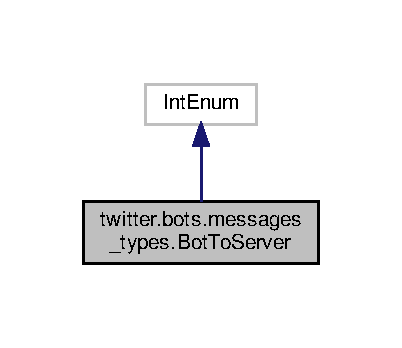
\includegraphics[width=193pt]{d3/d94/classtwitter_1_1bots_1_1messages__types_1_1BotToServer__inherit__graph}
\end{center}
\end{figure}


Collaboration diagram for twitter.\+bots.\+messages\+\_\+types.\+Bot\+To\+Server\+:\nopagebreak
\begin{figure}[H]
\begin{center}
\leavevmode
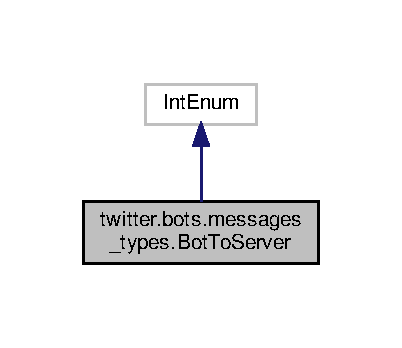
\includegraphics[width=193pt]{d0/dad/classtwitter_1_1bots_1_1messages__types_1_1BotToServer__coll__graph}
\end{center}
\end{figure}
\subsection*{Public Member Functions}
\begin{DoxyCompactItemize}
\item 
\mbox{\Hypertarget{classtwitter_1_1bots_1_1messages__types_1_1BotToServer_a915f4adbd233145618c2deec2c13e4eb}\label{classtwitter_1_1bots_1_1messages__types_1_1BotToServer_a915f4adbd233145618c2deec2c13e4eb}} 
def {\bfseries \+\_\+\+\_\+str\+\_\+\+\_\+} (self)
\end{DoxyCompactItemize}
\subsection*{Static Public Attributes}
\begin{DoxyCompactItemize}
\item 
\mbox{\Hypertarget{classtwitter_1_1bots_1_1messages__types_1_1BotToServer_abdaebceaf5179a32ed5319dc969326f0}\label{classtwitter_1_1bots_1_1messages__types_1_1BotToServer_abdaebceaf5179a32ed5319dc969326f0}} 
int {\bfseries E\+V\+E\+N\+T\+\_\+\+U\+S\+E\+R\+\_\+\+F\+O\+L\+L\+O\+W\+ED} = 1
\item 
\mbox{\Hypertarget{classtwitter_1_1bots_1_1messages__types_1_1BotToServer_aaeaf2710b539578b584abe78ceed5031}\label{classtwitter_1_1bots_1_1messages__types_1_1BotToServer_aaeaf2710b539578b584abe78ceed5031}} 
int {\bfseries E\+V\+E\+N\+T\+\_\+\+T\+W\+E\+E\+T\+\_\+\+L\+I\+K\+ED} = 2
\item 
\mbox{\Hypertarget{classtwitter_1_1bots_1_1messages__types_1_1BotToServer_a6df7456bdd9985bbb9e801fceb7c3cee}\label{classtwitter_1_1bots_1_1messages__types_1_1BotToServer_a6df7456bdd9985bbb9e801fceb7c3cee}} 
int {\bfseries E\+V\+E\+N\+T\+\_\+\+T\+W\+E\+E\+T\+\_\+\+R\+E\+T\+W\+E\+E\+T\+ED} = 3
\item 
\mbox{\Hypertarget{classtwitter_1_1bots_1_1messages__types_1_1BotToServer_a1201f51b73028bd56c920863a93aaefa}\label{classtwitter_1_1bots_1_1messages__types_1_1BotToServer_a1201f51b73028bd56c920863a93aaefa}} 
int {\bfseries E\+V\+E\+N\+T\+\_\+\+T\+W\+E\+E\+T\+\_\+\+R\+E\+P\+L\+I\+ED} = 4
\item 
\mbox{\Hypertarget{classtwitter_1_1bots_1_1messages__types_1_1BotToServer_a3c73fb1a6f014c96ed8dca3c39c86572}\label{classtwitter_1_1bots_1_1messages__types_1_1BotToServer_a3c73fb1a6f014c96ed8dca3c39c86572}} 
int {\bfseries Q\+U\+E\+R\+Y\+\_\+\+T\+W\+E\+E\+T\+\_\+\+L\+I\+KE} = 5
\item 
\mbox{\Hypertarget{classtwitter_1_1bots_1_1messages__types_1_1BotToServer_ad0cc59dfb250134e448e53fe37eb29e3}\label{classtwitter_1_1bots_1_1messages__types_1_1BotToServer_ad0cc59dfb250134e448e53fe37eb29e3}} 
int {\bfseries Q\+U\+E\+R\+Y\+\_\+\+T\+W\+E\+E\+T\+\_\+\+R\+E\+T\+W\+E\+ET} = 6
\item 
\mbox{\Hypertarget{classtwitter_1_1bots_1_1messages__types_1_1BotToServer_a34b0c9518de19c77dec3064bf75a1b52}\label{classtwitter_1_1bots_1_1messages__types_1_1BotToServer_a34b0c9518de19c77dec3064bf75a1b52}} 
int {\bfseries Q\+U\+E\+R\+Y\+\_\+\+T\+W\+E\+E\+T\+\_\+\+R\+E\+P\+LY} = 7
\item 
\mbox{\Hypertarget{classtwitter_1_1bots_1_1messages__types_1_1BotToServer_ae59feacd2e18ec6f834fab1c78fcaf5b}\label{classtwitter_1_1bots_1_1messages__types_1_1BotToServer_ae59feacd2e18ec6f834fab1c78fcaf5b}} 
int {\bfseries Q\+U\+E\+R\+Y\+\_\+\+F\+O\+L\+L\+O\+W\+\_\+\+U\+S\+ER} = 8
\item 
\mbox{\Hypertarget{classtwitter_1_1bots_1_1messages__types_1_1BotToServer_a56395fa1744d9e0cc651db321dbba982}\label{classtwitter_1_1bots_1_1messages__types_1_1BotToServer_a56395fa1744d9e0cc651db321dbba982}} 
int {\bfseries S\+A\+V\+E\+\_\+\+U\+S\+ER} = 9
\item 
\mbox{\Hypertarget{classtwitter_1_1bots_1_1messages__types_1_1BotToServer_a2d5b514d5acd789996554334b6400168}\label{classtwitter_1_1bots_1_1messages__types_1_1BotToServer_a2d5b514d5acd789996554334b6400168}} 
int {\bfseries S\+A\+V\+E\+\_\+\+T\+W\+E\+ET} = 10
\item 
\mbox{\Hypertarget{classtwitter_1_1bots_1_1messages__types_1_1BotToServer_a8a6114726265b63d224fe3c0bb22e327}\label{classtwitter_1_1bots_1_1messages__types_1_1BotToServer_a8a6114726265b63d224fe3c0bb22e327}} 
int {\bfseries E\+V\+E\+N\+T\+\_\+\+U\+S\+E\+R\+\_\+\+B\+L\+O\+C\+K\+ED} = 11
\item 
\mbox{\Hypertarget{classtwitter_1_1bots_1_1messages__types_1_1BotToServer_a142b0d8e3ee184b8a6ad1283ca23ad7a}\label{classtwitter_1_1bots_1_1messages__types_1_1BotToServer_a142b0d8e3ee184b8a6ad1283ca23ad7a}} 
int {\bfseries S\+A\+V\+E\+\_\+\+F\+O\+L\+L\+O\+W\+E\+RS} = 12
\item 
\mbox{\Hypertarget{classtwitter_1_1bots_1_1messages__types_1_1BotToServer_a0bbf4b687a54dca2b3ab3b4c6c01cc4a}\label{classtwitter_1_1bots_1_1messages__types_1_1BotToServer_a0bbf4b687a54dca2b3ab3b4c6c01cc4a}} 
int {\bfseries S\+A\+V\+E\+\_\+\+D\+I\+R\+E\+C\+T\+\_\+\+M\+E\+S\+S\+A\+G\+ES} = 13
\end{DoxyCompactItemize}


\subsection{Detailed Description}
Enum for the Messages sent by the bot to the server. 

The documentation for this class was generated from the following file\+:\begin{DoxyCompactItemize}
\item 
bots/messages\+\_\+types.\+py\end{DoxyCompactItemize}

\hypertarget{classtwitter_1_1control__center_1_1dbwriter_1_1DBWriter}{}\section{twitter.\+control\+\_\+center.\+dbwriter.\+D\+B\+Writer Class Reference}
\label{classtwitter_1_1control__center_1_1dbwriter_1_1DBWriter}\index{twitter.\+control\+\_\+center.\+dbwriter.\+D\+B\+Writer@{twitter.\+control\+\_\+center.\+dbwriter.\+D\+B\+Writer}}


Inheritance diagram for twitter.\+control\+\_\+center.\+dbwriter.\+D\+B\+Writer\+:
\nopagebreak
\begin{figure}[H]
\begin{center}
\leavevmode
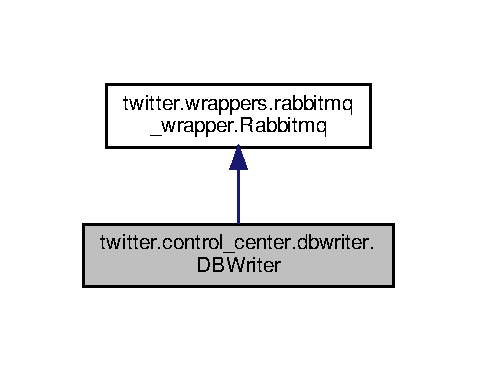
\includegraphics[width=229pt]{classtwitter_1_1control__center_1_1dbwriter_1_1DBWriter__inherit__graph}
\end{center}
\end{figure}


Collaboration diagram for twitter.\+control\+\_\+center.\+dbwriter.\+D\+B\+Writer\+:
\nopagebreak
\begin{figure}[H]
\begin{center}
\leavevmode
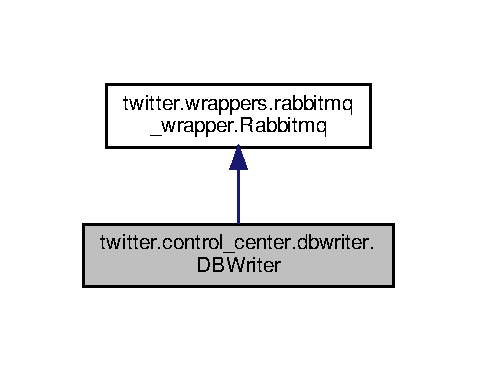
\includegraphics[width=229pt]{classtwitter_1_1control__center_1_1dbwriter_1_1DBWriter__coll__graph}
\end{center}
\end{figure}
\subsection*{Public Member Functions}
\begin{DoxyCompactItemize}
\item 
def \hyperlink{classtwitter_1_1control__center_1_1dbwriter_1_1DBWriter_a084c7286de1162ebb245a955a65e3911}{\+\_\+\+\_\+init\+\_\+\+\_\+} (self)
\item 
\mbox{\Hypertarget{classtwitter_1_1control__center_1_1dbwriter_1_1DBWriter_a87d9173e78b04aa21fac689879b5a3b3}\label{classtwitter_1_1control__center_1_1dbwriter_1_1DBWriter_a87d9173e78b04aa21fac689879b5a3b3}} 
def {\bfseries action} (self, message)
\item 
def \hyperlink{classtwitter_1_1control__center_1_1dbwriter_1_1DBWriter_a59e9de0b9462c07bc173e160c3431e5a}{follow\+\_\+user} (self, data)
\item 
def \hyperlink{classtwitter_1_1control__center_1_1dbwriter_1_1DBWriter_a4539c991b82dd529602cbd13d21a89b4}{like\+\_\+tweet} (self, data)
\item 
def \hyperlink{classtwitter_1_1control__center_1_1dbwriter_1_1DBWriter_a840d1892b618a29a5e44305cb6aa0211}{retweet} (self, data)
\item 
def \hyperlink{classtwitter_1_1control__center_1_1dbwriter_1_1DBWriter_a1005772e640f1c4aae538a7850c2d15d}{reply\+\_\+tweet} (self, data)
\item 
def \hyperlink{classtwitter_1_1control__center_1_1dbwriter_1_1DBWriter_acb9c768e2862639056ef226e2eab77ec}{request\+\_\+tweet\+\_\+like} (self, data)
\item 
def \hyperlink{classtwitter_1_1control__center_1_1dbwriter_1_1DBWriter_af94a869d95d271c9fc1d23b9281c95a9}{request\+\_\+retweet} (self, data)
\item 
def \hyperlink{classtwitter_1_1control__center_1_1dbwriter_1_1DBWriter_a876d7b694fb3f54940e7f07afcbb0c09}{request\+\_\+tweet\+\_\+reply} (self, data)
\item 
def \hyperlink{classtwitter_1_1control__center_1_1dbwriter_1_1DBWriter_a957daaa2da31d56fc7dccb9a18f3346d}{request\+\_\+follow\+\_\+user} (self, data)
\item 
def \hyperlink{classtwitter_1_1control__center_1_1dbwriter_1_1DBWriter_a38708a33bd2b8019383571275b8a0f17}{save\+\_\+user} (self, data)
\item 
def \hyperlink{classtwitter_1_1control__center_1_1dbwriter_1_1DBWriter_a0596d9924189129c588b6c603f462d5b}{save\+\_\+tweet} (self, data)
\item 
def \hyperlink{classtwitter_1_1control__center_1_1dbwriter_1_1DBWriter_a6b55377307e8c59054e0f136942c4a79}{save\+\_\+dm} (self, data)
\item 
def \hyperlink{classtwitter_1_1control__center_1_1dbwriter_1_1DBWriter_aa6e8cefc09b703abee2c4b3a68d62fd1}{error} (self, data)
\item 
def \hyperlink{classtwitter_1_1control__center_1_1dbwriter_1_1DBWriter_a65e268dcff959f29e258113ef6043a76}{find\+\_\+followers} (self, data)
\item 
def \hyperlink{classtwitter_1_1control__center_1_1dbwriter_1_1DBWriter_a3a6e2d36449a7f745d31e328cc4d92d9}{send} (self, bot, message\+\_\+type, params)
\item 
\mbox{\Hypertarget{classtwitter_1_1control__center_1_1dbwriter_1_1DBWriter_aa12d98995c446702bb434fff2e6ee0fd}\label{classtwitter_1_1control__center_1_1dbwriter_1_1DBWriter_aa12d98995c446702bb434fff2e6ee0fd}} 
def {\bfseries received\+\_\+message\+\_\+handler} (self, channel, method, properties, body)
\item 
\mbox{\Hypertarget{classtwitter_1_1control__center_1_1dbwriter_1_1DBWriter_a6236ff72370378d82719e4a74e120923}\label{classtwitter_1_1control__center_1_1dbwriter_1_1DBWriter_a6236ff72370378d82719e4a74e120923}} 
def {\bfseries run} (self)
\item 
\mbox{\Hypertarget{classtwitter_1_1control__center_1_1dbwriter_1_1DBWriter_aa06680faca4d475457fe1d19d95959ca}\label{classtwitter_1_1control__center_1_1dbwriter_1_1DBWriter_aa06680faca4d475457fe1d19d95959ca}} 
def {\bfseries close} (self)
\end{DoxyCompactItemize}
\subsection*{Public Attributes}
\begin{DoxyCompactItemize}
\item 
\mbox{\Hypertarget{classtwitter_1_1control__center_1_1dbwriter_1_1DBWriter_a6473c85a2b62791269ee42ce1731513c}\label{classtwitter_1_1control__center_1_1dbwriter_1_1DBWriter_a6473c85a2b62791269ee42ce1731513c}} 
{\bfseries postgress\+\_\+client}
\item 
\mbox{\Hypertarget{classtwitter_1_1control__center_1_1dbwriter_1_1DBWriter_acd3d98d13d85fb9335b8d4e9c866a2ab}\label{classtwitter_1_1control__center_1_1dbwriter_1_1DBWriter_acd3d98d13d85fb9335b8d4e9c866a2ab}} 
{\bfseries mongo\+\_\+client}
\item 
\mbox{\Hypertarget{classtwitter_1_1control__center_1_1dbwriter_1_1DBWriter_a5375348c728a40d18617e644d4aa1c39}\label{classtwitter_1_1control__center_1_1dbwriter_1_1DBWriter_a5375348c728a40d18617e644d4aa1c39}} 
{\bfseries neo4j\+\_\+client}
\item 
\mbox{\Hypertarget{classtwitter_1_1control__center_1_1dbwriter_1_1DBWriter_a531422c00b00ab64a2ad93133bc0e4d2}\label{classtwitter_1_1control__center_1_1dbwriter_1_1DBWriter_a531422c00b00ab64a2ad93133bc0e4d2}} 
{\bfseries pep}
\end{DoxyCompactItemize}


\subsection{Detailed Description}
\begin{DoxyVerb}Class to smulate the behaviour of a bot:
On receiving a message from a message broker, this class will act accordingly
\end{DoxyVerb}
 

\subsection{Constructor \& Destructor Documentation}
\mbox{\Hypertarget{classtwitter_1_1control__center_1_1dbwriter_1_1DBWriter_a084c7286de1162ebb245a955a65e3911}\label{classtwitter_1_1control__center_1_1dbwriter_1_1DBWriter_a084c7286de1162ebb245a955a65e3911}} 
\index{twitter\+::control\+\_\+center\+::dbwriter\+::\+D\+B\+Writer@{twitter\+::control\+\_\+center\+::dbwriter\+::\+D\+B\+Writer}!\+\_\+\+\_\+init\+\_\+\+\_\+@{\+\_\+\+\_\+init\+\_\+\+\_\+}}
\index{\+\_\+\+\_\+init\+\_\+\+\_\+@{\+\_\+\+\_\+init\+\_\+\+\_\+}!twitter\+::control\+\_\+center\+::dbwriter\+::\+D\+B\+Writer@{twitter\+::control\+\_\+center\+::dbwriter\+::\+D\+B\+Writer}}
\subsubsection{\texorpdfstring{\+\_\+\+\_\+init\+\_\+\+\_\+()}{\_\_init\_\_()}}
{\footnotesize\ttfamily def twitter.\+control\+\_\+center.\+dbwriter.\+D\+B\+Writer.\+\_\+\+\_\+init\+\_\+\+\_\+ (\begin{DoxyParamCaption}\item[{}]{self }\end{DoxyParamCaption})}

\begin{DoxyVerb}This will start instaces for all the DB's API
\end{DoxyVerb}
 

\subsection{Member Function Documentation}
\mbox{\Hypertarget{classtwitter_1_1control__center_1_1dbwriter_1_1DBWriter_aa6e8cefc09b703abee2c4b3a68d62fd1}\label{classtwitter_1_1control__center_1_1dbwriter_1_1DBWriter_aa6e8cefc09b703abee2c4b3a68d62fd1}} 
\index{twitter\+::control\+\_\+center\+::dbwriter\+::\+D\+B\+Writer@{twitter\+::control\+\_\+center\+::dbwriter\+::\+D\+B\+Writer}!error@{error}}
\index{error@{error}!twitter\+::control\+\_\+center\+::dbwriter\+::\+D\+B\+Writer@{twitter\+::control\+\_\+center\+::dbwriter\+::\+D\+B\+Writer}}
\subsubsection{\texorpdfstring{error()}{error()}}
{\footnotesize\ttfamily def twitter.\+control\+\_\+center.\+dbwriter.\+D\+B\+Writer.\+error (\begin{DoxyParamCaption}\item[{}]{self,  }\item[{}]{data }\end{DoxyParamCaption})}

\begin{DoxyVerb}Stores error that may have occured in the running of a bot:
Calls the postgres stats to log the error

@param data: dict with the id of a bot and the error object
\end{DoxyVerb}
 \mbox{\Hypertarget{classtwitter_1_1control__center_1_1dbwriter_1_1DBWriter_a65e268dcff959f29e258113ef6043a76}\label{classtwitter_1_1control__center_1_1dbwriter_1_1DBWriter_a65e268dcff959f29e258113ef6043a76}} 
\index{twitter\+::control\+\_\+center\+::dbwriter\+::\+D\+B\+Writer@{twitter\+::control\+\_\+center\+::dbwriter\+::\+D\+B\+Writer}!find\+\_\+followers@{find\+\_\+followers}}
\index{find\+\_\+followers@{find\+\_\+followers}!twitter\+::control\+\_\+center\+::dbwriter\+::\+D\+B\+Writer@{twitter\+::control\+\_\+center\+::dbwriter\+::\+D\+B\+Writer}}
\subsubsection{\texorpdfstring{find\+\_\+followers()}{find\_followers()}}
{\footnotesize\ttfamily def twitter.\+control\+\_\+center.\+dbwriter.\+D\+B\+Writer.\+find\+\_\+followers (\begin{DoxyParamCaption}\item[{}]{self,  }\item[{}]{data }\end{DoxyParamCaption})}

\begin{DoxyVerb}Function that writes the follow relationship on the Neo4j API database;
The function will also request for the bot who sent the message to follow the users who follow
one of the bot's followers

@param data: dict with the id of a bot and a second dictionary with the bot's followers' ID as keys that map
to his followers
\end{DoxyVerb}
 \mbox{\Hypertarget{classtwitter_1_1control__center_1_1dbwriter_1_1DBWriter_a59e9de0b9462c07bc173e160c3431e5a}\label{classtwitter_1_1control__center_1_1dbwriter_1_1DBWriter_a59e9de0b9462c07bc173e160c3431e5a}} 
\index{twitter\+::control\+\_\+center\+::dbwriter\+::\+D\+B\+Writer@{twitter\+::control\+\_\+center\+::dbwriter\+::\+D\+B\+Writer}!follow\+\_\+user@{follow\+\_\+user}}
\index{follow\+\_\+user@{follow\+\_\+user}!twitter\+::control\+\_\+center\+::dbwriter\+::\+D\+B\+Writer@{twitter\+::control\+\_\+center\+::dbwriter\+::\+D\+B\+Writer}}
\subsubsection{\texorpdfstring{follow\+\_\+user()}{follow\_user()}}
{\footnotesize\ttfamily def twitter.\+control\+\_\+center.\+dbwriter.\+D\+B\+Writer.\+follow\+\_\+user (\begin{DoxyParamCaption}\item[{}]{self,  }\item[{}]{data }\end{DoxyParamCaption})}

\begin{DoxyVerb}Action to follow user:
Calls neo4j to add new relation between bot and user
Calls postgres_stats to add new log with the action details

@param data: dict containing bot and the user he's following
\end{DoxyVerb}
 \mbox{\Hypertarget{classtwitter_1_1control__center_1_1dbwriter_1_1DBWriter_a4539c991b82dd529602cbd13d21a89b4}\label{classtwitter_1_1control__center_1_1dbwriter_1_1DBWriter_a4539c991b82dd529602cbd13d21a89b4}} 
\index{twitter\+::control\+\_\+center\+::dbwriter\+::\+D\+B\+Writer@{twitter\+::control\+\_\+center\+::dbwriter\+::\+D\+B\+Writer}!like\+\_\+tweet@{like\+\_\+tweet}}
\index{like\+\_\+tweet@{like\+\_\+tweet}!twitter\+::control\+\_\+center\+::dbwriter\+::\+D\+B\+Writer@{twitter\+::control\+\_\+center\+::dbwriter\+::\+D\+B\+Writer}}
\subsubsection{\texorpdfstring{like\+\_\+tweet()}{like\_tweet()}}
{\footnotesize\ttfamily def twitter.\+control\+\_\+center.\+dbwriter.\+D\+B\+Writer.\+like\+\_\+tweet (\begin{DoxyParamCaption}\item[{}]{self,  }\item[{}]{data }\end{DoxyParamCaption})}

\begin{DoxyVerb}Action to like tweet:
Calls postgres_stats to add new log

@param data dict with the bot id and the tweet he liked
\end{DoxyVerb}
 \mbox{\Hypertarget{classtwitter_1_1control__center_1_1dbwriter_1_1DBWriter_a1005772e640f1c4aae538a7850c2d15d}\label{classtwitter_1_1control__center_1_1dbwriter_1_1DBWriter_a1005772e640f1c4aae538a7850c2d15d}} 
\index{twitter\+::control\+\_\+center\+::dbwriter\+::\+D\+B\+Writer@{twitter\+::control\+\_\+center\+::dbwriter\+::\+D\+B\+Writer}!reply\+\_\+tweet@{reply\+\_\+tweet}}
\index{reply\+\_\+tweet@{reply\+\_\+tweet}!twitter\+::control\+\_\+center\+::dbwriter\+::\+D\+B\+Writer@{twitter\+::control\+\_\+center\+::dbwriter\+::\+D\+B\+Writer}}
\subsubsection{\texorpdfstring{reply\+\_\+tweet()}{reply\_tweet()}}
{\footnotesize\ttfamily def twitter.\+control\+\_\+center.\+dbwriter.\+D\+B\+Writer.\+reply\+\_\+tweet (\begin{DoxyParamCaption}\item[{}]{self,  }\item[{}]{data }\end{DoxyParamCaption})}

\begin{DoxyVerb}Action to reply a tweet:
Calls progres_stats to add what the bot replied and to which tweet

@param data: dict contaning bot and the reply they made
\end{DoxyVerb}
 \mbox{\Hypertarget{classtwitter_1_1control__center_1_1dbwriter_1_1DBWriter_a957daaa2da31d56fc7dccb9a18f3346d}\label{classtwitter_1_1control__center_1_1dbwriter_1_1DBWriter_a957daaa2da31d56fc7dccb9a18f3346d}} 
\index{twitter\+::control\+\_\+center\+::dbwriter\+::\+D\+B\+Writer@{twitter\+::control\+\_\+center\+::dbwriter\+::\+D\+B\+Writer}!request\+\_\+follow\+\_\+user@{request\+\_\+follow\+\_\+user}}
\index{request\+\_\+follow\+\_\+user@{request\+\_\+follow\+\_\+user}!twitter\+::control\+\_\+center\+::dbwriter\+::\+D\+B\+Writer@{twitter\+::control\+\_\+center\+::dbwriter\+::\+D\+B\+Writer}}
\subsubsection{\texorpdfstring{request\+\_\+follow\+\_\+user()}{request\_follow\_user()}}
{\footnotesize\ttfamily def twitter.\+control\+\_\+center.\+dbwriter.\+D\+B\+Writer.\+request\+\_\+follow\+\_\+user (\begin{DoxyParamCaption}\item[{}]{self,  }\item[{}]{data }\end{DoxyParamCaption})}

\begin{DoxyVerb}Action to request a follow:
Calls the control center to request the follow
Adds the log to postgres_stats, for the request and its result
The result is based on the Policy API object

@param data: dict containing the bot id and the tweet id
\end{DoxyVerb}
 \mbox{\Hypertarget{classtwitter_1_1control__center_1_1dbwriter_1_1DBWriter_af94a869d95d271c9fc1d23b9281c95a9}\label{classtwitter_1_1control__center_1_1dbwriter_1_1DBWriter_af94a869d95d271c9fc1d23b9281c95a9}} 
\index{twitter\+::control\+\_\+center\+::dbwriter\+::\+D\+B\+Writer@{twitter\+::control\+\_\+center\+::dbwriter\+::\+D\+B\+Writer}!request\+\_\+retweet@{request\+\_\+retweet}}
\index{request\+\_\+retweet@{request\+\_\+retweet}!twitter\+::control\+\_\+center\+::dbwriter\+::\+D\+B\+Writer@{twitter\+::control\+\_\+center\+::dbwriter\+::\+D\+B\+Writer}}
\subsubsection{\texorpdfstring{request\+\_\+retweet()}{request\_retweet()}}
{\footnotesize\ttfamily def twitter.\+control\+\_\+center.\+dbwriter.\+D\+B\+Writer.\+request\+\_\+retweet (\begin{DoxyParamCaption}\item[{}]{self,  }\item[{}]{data }\end{DoxyParamCaption})}

\begin{DoxyVerb}Action to request a retweet:
Calls the PEP to request the retweet
Adds the log to postgres_stats, for the request and its result
The result is based on the PDP methods

2param data: dict containing the bot id and the tweet id
\end{DoxyVerb}
 \mbox{\Hypertarget{classtwitter_1_1control__center_1_1dbwriter_1_1DBWriter_acb9c768e2862639056ef226e2eab77ec}\label{classtwitter_1_1control__center_1_1dbwriter_1_1DBWriter_acb9c768e2862639056ef226e2eab77ec}} 
\index{twitter\+::control\+\_\+center\+::dbwriter\+::\+D\+B\+Writer@{twitter\+::control\+\_\+center\+::dbwriter\+::\+D\+B\+Writer}!request\+\_\+tweet\+\_\+like@{request\+\_\+tweet\+\_\+like}}
\index{request\+\_\+tweet\+\_\+like@{request\+\_\+tweet\+\_\+like}!twitter\+::control\+\_\+center\+::dbwriter\+::\+D\+B\+Writer@{twitter\+::control\+\_\+center\+::dbwriter\+::\+D\+B\+Writer}}
\subsubsection{\texorpdfstring{request\+\_\+tweet\+\_\+like()}{request\_tweet\_like()}}
{\footnotesize\ttfamily def twitter.\+control\+\_\+center.\+dbwriter.\+D\+B\+Writer.\+request\+\_\+tweet\+\_\+like (\begin{DoxyParamCaption}\item[{}]{self,  }\item[{}]{data }\end{DoxyParamCaption})}

\begin{DoxyVerb}Action to request a like on tweeter:
Calls the PEP to request a like
Adds the log to postgres_stats, for the request and its result
The result is based on the PDP methods

@param data: dict containing the bot id and the tweet id
\end{DoxyVerb}
 \mbox{\Hypertarget{classtwitter_1_1control__center_1_1dbwriter_1_1DBWriter_a876d7b694fb3f54940e7f07afcbb0c09}\label{classtwitter_1_1control__center_1_1dbwriter_1_1DBWriter_a876d7b694fb3f54940e7f07afcbb0c09}} 
\index{twitter\+::control\+\_\+center\+::dbwriter\+::\+D\+B\+Writer@{twitter\+::control\+\_\+center\+::dbwriter\+::\+D\+B\+Writer}!request\+\_\+tweet\+\_\+reply@{request\+\_\+tweet\+\_\+reply}}
\index{request\+\_\+tweet\+\_\+reply@{request\+\_\+tweet\+\_\+reply}!twitter\+::control\+\_\+center\+::dbwriter\+::\+D\+B\+Writer@{twitter\+::control\+\_\+center\+::dbwriter\+::\+D\+B\+Writer}}
\subsubsection{\texorpdfstring{request\+\_\+tweet\+\_\+reply()}{request\_tweet\_reply()}}
{\footnotesize\ttfamily def twitter.\+control\+\_\+center.\+dbwriter.\+D\+B\+Writer.\+request\+\_\+tweet\+\_\+reply (\begin{DoxyParamCaption}\item[{}]{self,  }\item[{}]{data }\end{DoxyParamCaption})}

\begin{DoxyVerb}Action to request a reply:
Calls the control center to request the reply
Adds the log to postgres_stats, for the request and its result
The result is based on the Policy API object

@param data: dict containing the bot id and the tweet id
\end{DoxyVerb}
 \mbox{\Hypertarget{classtwitter_1_1control__center_1_1dbwriter_1_1DBWriter_a840d1892b618a29a5e44305cb6aa0211}\label{classtwitter_1_1control__center_1_1dbwriter_1_1DBWriter_a840d1892b618a29a5e44305cb6aa0211}} 
\index{twitter\+::control\+\_\+center\+::dbwriter\+::\+D\+B\+Writer@{twitter\+::control\+\_\+center\+::dbwriter\+::\+D\+B\+Writer}!retweet@{retweet}}
\index{retweet@{retweet}!twitter\+::control\+\_\+center\+::dbwriter\+::\+D\+B\+Writer@{twitter\+::control\+\_\+center\+::dbwriter\+::\+D\+B\+Writer}}
\subsubsection{\texorpdfstring{retweet()}{retweet()}}
{\footnotesize\ttfamily def twitter.\+control\+\_\+center.\+dbwriter.\+D\+B\+Writer.\+retweet (\begin{DoxyParamCaption}\item[{}]{self,  }\item[{}]{data }\end{DoxyParamCaption})}

\begin{DoxyVerb}Action to retweet:
Calls postgres_stats to add new log

@param data: dict containing bot and the tweet he retweeted
\end{DoxyVerb}
 \mbox{\Hypertarget{classtwitter_1_1control__center_1_1dbwriter_1_1DBWriter_a6b55377307e8c59054e0f136942c4a79}\label{classtwitter_1_1control__center_1_1dbwriter_1_1DBWriter_a6b55377307e8c59054e0f136942c4a79}} 
\index{twitter\+::control\+\_\+center\+::dbwriter\+::\+D\+B\+Writer@{twitter\+::control\+\_\+center\+::dbwriter\+::\+D\+B\+Writer}!save\+\_\+dm@{save\+\_\+dm}}
\index{save\+\_\+dm@{save\+\_\+dm}!twitter\+::control\+\_\+center\+::dbwriter\+::\+D\+B\+Writer@{twitter\+::control\+\_\+center\+::dbwriter\+::\+D\+B\+Writer}}
\subsubsection{\texorpdfstring{save\+\_\+dm()}{save\_dm()}}
{\footnotesize\ttfamily def twitter.\+control\+\_\+center.\+dbwriter.\+D\+B\+Writer.\+save\+\_\+dm (\begin{DoxyParamCaption}\item[{}]{self,  }\item[{}]{data }\end{DoxyParamCaption})}

\begin{DoxyVerb}Stores the info about a bot's direct messages:
Calls the mongo object to save or update a dm
Adds the operation log to postgress_stats

@param data: dict containignt the id of the bot and the DMs
\end{DoxyVerb}
 \mbox{\Hypertarget{classtwitter_1_1control__center_1_1dbwriter_1_1DBWriter_a0596d9924189129c588b6c603f462d5b}\label{classtwitter_1_1control__center_1_1dbwriter_1_1DBWriter_a0596d9924189129c588b6c603f462d5b}} 
\index{twitter\+::control\+\_\+center\+::dbwriter\+::\+D\+B\+Writer@{twitter\+::control\+\_\+center\+::dbwriter\+::\+D\+B\+Writer}!save\+\_\+tweet@{save\+\_\+tweet}}
\index{save\+\_\+tweet@{save\+\_\+tweet}!twitter\+::control\+\_\+center\+::dbwriter\+::\+D\+B\+Writer@{twitter\+::control\+\_\+center\+::dbwriter\+::\+D\+B\+Writer}}
\subsubsection{\texorpdfstring{save\+\_\+tweet()}{save\_tweet()}}
{\footnotesize\ttfamily def twitter.\+control\+\_\+center.\+dbwriter.\+D\+B\+Writer.\+save\+\_\+tweet (\begin{DoxyParamCaption}\item[{}]{self,  }\item[{}]{data }\end{DoxyParamCaption})}

\begin{DoxyVerb}Stores info about a tweet:
Calls the mongo object to save or update a tweet
Adds the operation log to postgress_stats

@param data: dict containing the id of the tweet to bee saved
\end{DoxyVerb}
 \mbox{\Hypertarget{classtwitter_1_1control__center_1_1dbwriter_1_1DBWriter_a38708a33bd2b8019383571275b8a0f17}\label{classtwitter_1_1control__center_1_1dbwriter_1_1DBWriter_a38708a33bd2b8019383571275b8a0f17}} 
\index{twitter\+::control\+\_\+center\+::dbwriter\+::\+D\+B\+Writer@{twitter\+::control\+\_\+center\+::dbwriter\+::\+D\+B\+Writer}!save\+\_\+user@{save\+\_\+user}}
\index{save\+\_\+user@{save\+\_\+user}!twitter\+::control\+\_\+center\+::dbwriter\+::\+D\+B\+Writer@{twitter\+::control\+\_\+center\+::dbwriter\+::\+D\+B\+Writer}}
\subsubsection{\texorpdfstring{save\+\_\+user()}{save\_user()}}
{\footnotesize\ttfamily def twitter.\+control\+\_\+center.\+dbwriter.\+D\+B\+Writer.\+save\+\_\+user (\begin{DoxyParamCaption}\item[{}]{self,  }\item[{}]{data }\end{DoxyParamCaption})}

\begin{DoxyVerb}Stores info about a user:
Calls the neo4j and the mongo object to update or store the user be it a bot or a user)
Adds the log of the operation to postgress_stats
If the user is a bot, must also call the Policy API object

@param data: dict containing the id of the bot and the user object
\end{DoxyVerb}
 \mbox{\Hypertarget{classtwitter_1_1control__center_1_1dbwriter_1_1DBWriter_a3a6e2d36449a7f745d31e328cc4d92d9}\label{classtwitter_1_1control__center_1_1dbwriter_1_1DBWriter_a3a6e2d36449a7f745d31e328cc4d92d9}} 
\index{twitter\+::control\+\_\+center\+::dbwriter\+::\+D\+B\+Writer@{twitter\+::control\+\_\+center\+::dbwriter\+::\+D\+B\+Writer}!send@{send}}
\index{send@{send}!twitter\+::control\+\_\+center\+::dbwriter\+::\+D\+B\+Writer@{twitter\+::control\+\_\+center\+::dbwriter\+::\+D\+B\+Writer}}
\subsubsection{\texorpdfstring{send()}{send()}}
{\footnotesize\ttfamily def twitter.\+control\+\_\+center.\+dbwriter.\+D\+B\+Writer.\+send (\begin{DoxyParamCaption}\item[{}]{self,  }\item[{}]{bot,  }\item[{}]{message\+\_\+type,  }\item[{}]{params }\end{DoxyParamCaption})}

\begin{DoxyVerb}Function the task uses to send messages through rabbit

@param bot: id of the bot to reply
@param message_type: ResponseTypes object with the type of message
@param params: dict with arguments of the message
\end{DoxyVerb}
 

The documentation for this class was generated from the following file\+:\begin{DoxyCompactItemize}
\item 
control\+\_\+center/dbwriter.\+py\end{DoxyCompactItemize}

\hypertarget{classtwitter_1_1control__center_1_1enums_1_1MessageTypes}{}\section{twitter.\+control\+\_\+center.\+enums.\+Message\+Types Class Reference}
\label{classtwitter_1_1control__center_1_1enums_1_1MessageTypes}\index{twitter.\+control\+\_\+center.\+enums.\+Message\+Types@{twitter.\+control\+\_\+center.\+enums.\+Message\+Types}}


Inheritance diagram for twitter.\+control\+\_\+center.\+enums.\+Message\+Types\+:\nopagebreak
\begin{figure}[H]
\begin{center}
\leavevmode
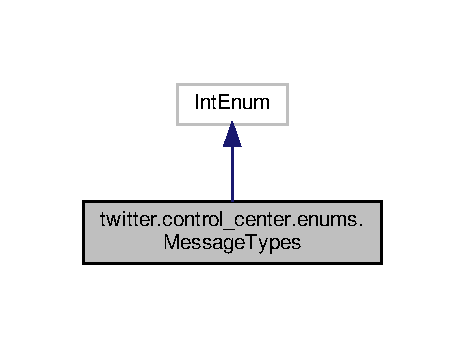
\includegraphics[width=223pt]{classtwitter_1_1control__center_1_1enums_1_1MessageTypes__inherit__graph}
\end{center}
\end{figure}


Collaboration diagram for twitter.\+control\+\_\+center.\+enums.\+Message\+Types\+:\nopagebreak
\begin{figure}[H]
\begin{center}
\leavevmode
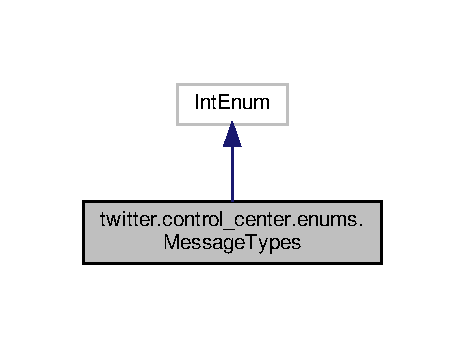
\includegraphics[width=223pt]{classtwitter_1_1control__center_1_1enums_1_1MessageTypes__coll__graph}
\end{center}
\end{figure}
\subsection*{Static Public Attributes}
\begin{DoxyCompactItemize}
\item 
\mbox{\Hypertarget{classtwitter_1_1control__center_1_1enums_1_1MessageTypes_ad79fd37d82f6b4c19cd27fa32a0a08af}\label{classtwitter_1_1control__center_1_1enums_1_1MessageTypes_ad79fd37d82f6b4c19cd27fa32a0a08af}} 
int {\bfseries U\+S\+E\+R\+\_\+\+F\+O\+L\+L\+O\+W\+ED} = 1
\item 
\mbox{\Hypertarget{classtwitter_1_1control__center_1_1enums_1_1MessageTypes_a68ae4e05328ea687336a2704a83121c2}\label{classtwitter_1_1control__center_1_1enums_1_1MessageTypes_a68ae4e05328ea687336a2704a83121c2}} 
int {\bfseries T\+W\+E\+E\+T\+\_\+\+L\+I\+K\+ED} = 2
\item 
\mbox{\Hypertarget{classtwitter_1_1control__center_1_1enums_1_1MessageTypes_abb665de212616bb5a0a7db321ba11d90}\label{classtwitter_1_1control__center_1_1enums_1_1MessageTypes_abb665de212616bb5a0a7db321ba11d90}} 
int {\bfseries T\+W\+E\+E\+T\+\_\+\+R\+E\+T\+W\+E\+E\+T\+D\+ED} = 3
\item 
\mbox{\Hypertarget{classtwitter_1_1control__center_1_1enums_1_1MessageTypes_a55ae42a86e57bd1954633976980dcedc}\label{classtwitter_1_1control__center_1_1enums_1_1MessageTypes_a55ae42a86e57bd1954633976980dcedc}} 
int {\bfseries T\+W\+E\+E\+T\+\_\+\+R\+E\+P\+L\+I\+ED} = 4
\item 
\mbox{\Hypertarget{classtwitter_1_1control__center_1_1enums_1_1MessageTypes_a289dcbb235f965944802e615c7577667}\label{classtwitter_1_1control__center_1_1enums_1_1MessageTypes_a289dcbb235f965944802e615c7577667}} 
int {\bfseries R\+E\+Q\+U\+E\+S\+T\+\_\+\+T\+W\+E\+E\+T\+\_\+\+L\+I\+KE} = 5
\item 
\mbox{\Hypertarget{classtwitter_1_1control__center_1_1enums_1_1MessageTypes_ac8aa8686ae09e334fe6d785db05f0b67}\label{classtwitter_1_1control__center_1_1enums_1_1MessageTypes_ac8aa8686ae09e334fe6d785db05f0b67}} 
int {\bfseries R\+E\+Q\+U\+E\+S\+T\+\_\+\+T\+W\+E\+E\+T\+\_\+\+R\+E\+T\+W\+E\+ET} = 6
\item 
\mbox{\Hypertarget{classtwitter_1_1control__center_1_1enums_1_1MessageTypes_aa6fd6edfe44dad7f2ec560be1c08988f}\label{classtwitter_1_1control__center_1_1enums_1_1MessageTypes_aa6fd6edfe44dad7f2ec560be1c08988f}} 
int {\bfseries R\+E\+Q\+U\+E\+S\+T\+\_\+\+T\+W\+E\+E\+T\+\_\+\+R\+E\+P\+LY} = 7
\item 
\mbox{\Hypertarget{classtwitter_1_1control__center_1_1enums_1_1MessageTypes_ac1debc137c3bdd350d47842824b1d510}\label{classtwitter_1_1control__center_1_1enums_1_1MessageTypes_ac1debc137c3bdd350d47842824b1d510}} 
int {\bfseries R\+E\+Q\+U\+E\+S\+T\+\_\+\+F\+O\+L\+L\+O\+W\+\_\+\+U\+S\+ER} = 8
\item 
\mbox{\Hypertarget{classtwitter_1_1control__center_1_1enums_1_1MessageTypes_a2a089d289ff787e4b83a1e3fc88f1cf6}\label{classtwitter_1_1control__center_1_1enums_1_1MessageTypes_a2a089d289ff787e4b83a1e3fc88f1cf6}} 
int {\bfseries S\+A\+V\+E\+\_\+\+U\+S\+ER} = 9
\item 
\mbox{\Hypertarget{classtwitter_1_1control__center_1_1enums_1_1MessageTypes_a51744590d4ab277af15967f673bd9f81}\label{classtwitter_1_1control__center_1_1enums_1_1MessageTypes_a51744590d4ab277af15967f673bd9f81}} 
int {\bfseries S\+A\+V\+E\+\_\+\+T\+W\+E\+ET} = 10
\item 
\mbox{\Hypertarget{classtwitter_1_1control__center_1_1enums_1_1MessageTypes_a5d28dcbde8f1cf73eeae72d5e4255fa9}\label{classtwitter_1_1control__center_1_1enums_1_1MessageTypes_a5d28dcbde8f1cf73eeae72d5e4255fa9}} 
int {\bfseries E\+R\+R\+O\+R\+\_\+\+B\+OT} = 11
\item 
\mbox{\Hypertarget{classtwitter_1_1control__center_1_1enums_1_1MessageTypes_a2a3ad2cdcd0a0a790e16e9c22103783c}\label{classtwitter_1_1control__center_1_1enums_1_1MessageTypes_a2a3ad2cdcd0a0a790e16e9c22103783c}} 
int {\bfseries F\+I\+N\+D\+\_\+\+F\+O\+L\+L\+O\+W\+E\+RS} = 12
\item 
\mbox{\Hypertarget{classtwitter_1_1control__center_1_1enums_1_1MessageTypes_a410903a67e59e67bfdf781e6ce0ce6e9}\label{classtwitter_1_1control__center_1_1enums_1_1MessageTypes_a410903a67e59e67bfdf781e6ce0ce6e9}} 
int {\bfseries S\+A\+V\+E\+\_\+\+D\+I\+R\+E\+C\+T\+\_\+\+M\+E\+S\+S\+A\+G\+ES} = 13
\end{DoxyCompactItemize}


The documentation for this class was generated from the following file\+:\begin{DoxyCompactItemize}
\item 
control\+\_\+center/enums.\+py\end{DoxyCompactItemize}

\hypertarget{classtwitter_1_1bots_1_1rabbit__messaging_1_1MessagingSettings}{}\section{twitter.\+bots.\+rabbit\+\_\+messaging.\+Messaging\+Settings Class Reference}
\label{classtwitter_1_1bots_1_1rabbit__messaging_1_1MessagingSettings}\index{twitter.\+bots.\+rabbit\+\_\+messaging.\+Messaging\+Settings@{twitter.\+bots.\+rabbit\+\_\+messaging.\+Messaging\+Settings}}
\subsection*{Public Member Functions}
\begin{DoxyCompactItemize}
\item 
\mbox{\Hypertarget{classtwitter_1_1bots_1_1rabbit__messaging_1_1MessagingSettings_aab02d3dd7fcb1ce90bdad005eea1ad03}\label{classtwitter_1_1bots_1_1rabbit__messaging_1_1MessagingSettings_aab02d3dd7fcb1ce90bdad005eea1ad03}} 
def {\bfseries \+\_\+\+\_\+init\+\_\+\+\_\+} (self, exchange, routing\+\_\+key, queue=None)
\item 
\mbox{\Hypertarget{classtwitter_1_1bots_1_1rabbit__messaging_1_1MessagingSettings_a30879baea8ee9148f80be7e3176af734}\label{classtwitter_1_1bots_1_1rabbit__messaging_1_1MessagingSettings_a30879baea8ee9148f80be7e3176af734}} 
def {\bfseries \+\_\+\+\_\+str\+\_\+\+\_\+} (self)
\end{DoxyCompactItemize}
\subsection*{Public Attributes}
\begin{DoxyCompactItemize}
\item 
\mbox{\Hypertarget{classtwitter_1_1bots_1_1rabbit__messaging_1_1MessagingSettings_a6d11f8ce4ea05f1309edbead3eb0f9fb}\label{classtwitter_1_1bots_1_1rabbit__messaging_1_1MessagingSettings_a6d11f8ce4ea05f1309edbead3eb0f9fb}} 
{\bfseries exchange}
\item 
\mbox{\Hypertarget{classtwitter_1_1bots_1_1rabbit__messaging_1_1MessagingSettings_a352277abd0a4593c8d7ba67e0ddd0b24}\label{classtwitter_1_1bots_1_1rabbit__messaging_1_1MessagingSettings_a352277abd0a4593c8d7ba67e0ddd0b24}} 
{\bfseries routing\+\_\+key}
\item 
\mbox{\Hypertarget{classtwitter_1_1bots_1_1rabbit__messaging_1_1MessagingSettings_a2b192d87a0cabd664183d20295297c5a}\label{classtwitter_1_1bots_1_1rabbit__messaging_1_1MessagingSettings_a2b192d87a0cabd664183d20295297c5a}} 
{\bfseries queue}
\end{DoxyCompactItemize}


The documentation for this class was generated from the following file\+:\begin{DoxyCompactItemize}
\item 
bots/rabbit\+\_\+messaging.\+py\end{DoxyCompactItemize}

\hypertarget{classtwitter_1_1wrappers_1_1mongo__wrapper_1_1MongoAPI}{}\section{twitter.\+wrappers.\+mongo\+\_\+wrapper.\+Mongo\+A\+PI Class Reference}
\label{classtwitter_1_1wrappers_1_1mongo__wrapper_1_1MongoAPI}\index{twitter.\+wrappers.\+mongo\+\_\+wrapper.\+Mongo\+A\+PI@{twitter.\+wrappers.\+mongo\+\_\+wrapper.\+Mongo\+A\+PI}}
\subsection*{Public Member Functions}
\begin{DoxyCompactItemize}
\item 
\mbox{\Hypertarget{classtwitter_1_1wrappers_1_1mongo__wrapper_1_1MongoAPI_afe7e92fefbe19be0561e810302fb4611}\label{classtwitter_1_1wrappers_1_1mongo__wrapper_1_1MongoAPI_afe7e92fefbe19be0561e810302fb4611}} 
def {\bfseries \+\_\+\+\_\+init\+\_\+\+\_\+} (self)
\item 
def \hyperlink{classtwitter_1_1wrappers_1_1mongo__wrapper_1_1MongoAPI_ad1adb6d5aa5e20cc43b77ab11d6403a3}{verify\+\_\+integrity} (self, collection, document)
\item 
def \hyperlink{classtwitter_1_1wrappers_1_1mongo__wrapper_1_1MongoAPI_a7c5d38f4ab2e2680224d47278b01d3bb}{get\+\_\+count} (self, collection, data=\{\})
\item 
def \hyperlink{classtwitter_1_1wrappers_1_1mongo__wrapper_1_1MongoAPI_a3f6edee30773ed114e48e32d54d45574}{insert\+\_\+users} (self, data)
\item 
def \hyperlink{classtwitter_1_1wrappers_1_1mongo__wrapper_1_1MongoAPI_a83f45c0a62f892db52f103756a523716}{insert\+\_\+tweets} (self, data)
\item 
def \hyperlink{classtwitter_1_1wrappers_1_1mongo__wrapper_1_1MongoAPI_af601222e36a6c0b6e131f788388ef992}{insert\+\_\+messages} (self, data)
\item 
def \hyperlink{classtwitter_1_1wrappers_1_1mongo__wrapper_1_1MongoAPI_aa4b9a6fb625844e6b78072b8818affd7}{update\+\_\+users} (self, match, new\+\_\+data, all=True)
\item 
def \hyperlink{classtwitter_1_1wrappers_1_1mongo__wrapper_1_1MongoAPI_a2b622e0eb9a3f45ecdf4b5f620f0231e}{update\+\_\+tweets} (self, match, new\+\_\+data, all=True)
\item 
def \hyperlink{classtwitter_1_1wrappers_1_1mongo__wrapper_1_1MongoAPI_a731dfdca8eac58b3b2b052e0a28bffcd}{update\+\_\+messages} (self, match, new\+\_\+data, all=True)
\item 
def \hyperlink{classtwitter_1_1wrappers_1_1mongo__wrapper_1_1MongoAPI_a6c5e6f8615e5795faffe3126b413dc05}{search} (self, collection, query=\{\}, fields=None, single=False, export\+\_\+type=None)
\end{DoxyCompactItemize}
\subsection*{Public Attributes}
\begin{DoxyCompactItemize}
\item 
\mbox{\Hypertarget{classtwitter_1_1wrappers_1_1mongo__wrapper_1_1MongoAPI_a67a94b824415d1f71214935251f77a58}\label{classtwitter_1_1wrappers_1_1mongo__wrapper_1_1MongoAPI_a67a94b824415d1f71214935251f77a58}} 
{\bfseries client}
\item 
\mbox{\Hypertarget{classtwitter_1_1wrappers_1_1mongo__wrapper_1_1MongoAPI_ad0c0cdc04fa5352dafc6f90f2e39b682}\label{classtwitter_1_1wrappers_1_1mongo__wrapper_1_1MongoAPI_ad0c0cdc04fa5352dafc6f90f2e39b682}} 
{\bfseries users}
\item 
\mbox{\Hypertarget{classtwitter_1_1wrappers_1_1mongo__wrapper_1_1MongoAPI_a47a3a708904c23154a9eee64b4b694c9}\label{classtwitter_1_1wrappers_1_1mongo__wrapper_1_1MongoAPI_a47a3a708904c23154a9eee64b4b694c9}} 
{\bfseries tweets}
\item 
\mbox{\Hypertarget{classtwitter_1_1wrappers_1_1mongo__wrapper_1_1MongoAPI_ad7ba1ef520ca7913137e8c2dcfbd26d4}\label{classtwitter_1_1wrappers_1_1mongo__wrapper_1_1MongoAPI_ad7ba1ef520ca7913137e8c2dcfbd26d4}} 
{\bfseries messages}
\end{DoxyCompactItemize}


\subsection{Detailed Description}
\begin{DoxyVerb}Mongo Wrapper.

Class that acts as a wrapper for all methods related to our Mongo DB
\end{DoxyVerb}
 

\subsection{Member Function Documentation}
\mbox{\Hypertarget{classtwitter_1_1wrappers_1_1mongo__wrapper_1_1MongoAPI_a7c5d38f4ab2e2680224d47278b01d3bb}\label{classtwitter_1_1wrappers_1_1mongo__wrapper_1_1MongoAPI_a7c5d38f4ab2e2680224d47278b01d3bb}} 
\index{twitter\+::wrappers\+::mongo\+\_\+wrapper\+::\+Mongo\+A\+PI@{twitter\+::wrappers\+::mongo\+\_\+wrapper\+::\+Mongo\+A\+PI}!get\+\_\+count@{get\+\_\+count}}
\index{get\+\_\+count@{get\+\_\+count}!twitter\+::wrappers\+::mongo\+\_\+wrapper\+::\+Mongo\+A\+PI@{twitter\+::wrappers\+::mongo\+\_\+wrapper\+::\+Mongo\+A\+PI}}
\subsubsection{\texorpdfstring{get\+\_\+count()}{get\_count()}}
{\footnotesize\ttfamily def twitter.\+wrappers.\+mongo\+\_\+wrapper.\+Mongo\+A\+P\+I.\+get\+\_\+count (\begin{DoxyParamCaption}\item[{}]{self,  }\item[{}]{collection,  }\item[{}]{data = {\ttfamily \{\}} }\end{DoxyParamCaption})}

\begin{DoxyVerb}Gets the total number of documents in a given collection

@param collection: The collection we want to count the documents in
@param data: The params we want the counted documents to have. By default it counts all documents
@return: The number of documents in a given collection
\end{DoxyVerb}
 \mbox{\Hypertarget{classtwitter_1_1wrappers_1_1mongo__wrapper_1_1MongoAPI_af601222e36a6c0b6e131f788388ef992}\label{classtwitter_1_1wrappers_1_1mongo__wrapper_1_1MongoAPI_af601222e36a6c0b6e131f788388ef992}} 
\index{twitter\+::wrappers\+::mongo\+\_\+wrapper\+::\+Mongo\+A\+PI@{twitter\+::wrappers\+::mongo\+\_\+wrapper\+::\+Mongo\+A\+PI}!insert\+\_\+messages@{insert\+\_\+messages}}
\index{insert\+\_\+messages@{insert\+\_\+messages}!twitter\+::wrappers\+::mongo\+\_\+wrapper\+::\+Mongo\+A\+PI@{twitter\+::wrappers\+::mongo\+\_\+wrapper\+::\+Mongo\+A\+PI}}
\subsubsection{\texorpdfstring{insert\+\_\+messages()}{insert\_messages()}}
{\footnotesize\ttfamily def twitter.\+wrappers.\+mongo\+\_\+wrapper.\+Mongo\+A\+P\+I.\+insert\+\_\+messages (\begin{DoxyParamCaption}\item[{}]{self,  }\item[{}]{data }\end{DoxyParamCaption})}

\begin{DoxyVerb}Inserts a new single document into our Messages Collection

@param data: The document to be inserted. Should be in the form of a dictionary
\end{DoxyVerb}
 \mbox{\Hypertarget{classtwitter_1_1wrappers_1_1mongo__wrapper_1_1MongoAPI_a83f45c0a62f892db52f103756a523716}\label{classtwitter_1_1wrappers_1_1mongo__wrapper_1_1MongoAPI_a83f45c0a62f892db52f103756a523716}} 
\index{twitter\+::wrappers\+::mongo\+\_\+wrapper\+::\+Mongo\+A\+PI@{twitter\+::wrappers\+::mongo\+\_\+wrapper\+::\+Mongo\+A\+PI}!insert\+\_\+tweets@{insert\+\_\+tweets}}
\index{insert\+\_\+tweets@{insert\+\_\+tweets}!twitter\+::wrappers\+::mongo\+\_\+wrapper\+::\+Mongo\+A\+PI@{twitter\+::wrappers\+::mongo\+\_\+wrapper\+::\+Mongo\+A\+PI}}
\subsubsection{\texorpdfstring{insert\+\_\+tweets()}{insert\_tweets()}}
{\footnotesize\ttfamily def twitter.\+wrappers.\+mongo\+\_\+wrapper.\+Mongo\+A\+P\+I.\+insert\+\_\+tweets (\begin{DoxyParamCaption}\item[{}]{self,  }\item[{}]{data }\end{DoxyParamCaption})}

\begin{DoxyVerb}Inserts a new single document into our Tweets Collection

@param data: The document to be inserted. Should be in the form of a dictionary
\end{DoxyVerb}
 \mbox{\Hypertarget{classtwitter_1_1wrappers_1_1mongo__wrapper_1_1MongoAPI_a3f6edee30773ed114e48e32d54d45574}\label{classtwitter_1_1wrappers_1_1mongo__wrapper_1_1MongoAPI_a3f6edee30773ed114e48e32d54d45574}} 
\index{twitter\+::wrappers\+::mongo\+\_\+wrapper\+::\+Mongo\+A\+PI@{twitter\+::wrappers\+::mongo\+\_\+wrapper\+::\+Mongo\+A\+PI}!insert\+\_\+users@{insert\+\_\+users}}
\index{insert\+\_\+users@{insert\+\_\+users}!twitter\+::wrappers\+::mongo\+\_\+wrapper\+::\+Mongo\+A\+PI@{twitter\+::wrappers\+::mongo\+\_\+wrapper\+::\+Mongo\+A\+PI}}
\subsubsection{\texorpdfstring{insert\+\_\+users()}{insert\_users()}}
{\footnotesize\ttfamily def twitter.\+wrappers.\+mongo\+\_\+wrapper.\+Mongo\+A\+P\+I.\+insert\+\_\+users (\begin{DoxyParamCaption}\item[{}]{self,  }\item[{}]{data }\end{DoxyParamCaption})}

\begin{DoxyVerb}Inserts a new single document into our Users Collection

@param data: The document to be inserted. Should be in the form of a dictionary
\end{DoxyVerb}
 \mbox{\Hypertarget{classtwitter_1_1wrappers_1_1mongo__wrapper_1_1MongoAPI_a6c5e6f8615e5795faffe3126b413dc05}\label{classtwitter_1_1wrappers_1_1mongo__wrapper_1_1MongoAPI_a6c5e6f8615e5795faffe3126b413dc05}} 
\index{twitter\+::wrappers\+::mongo\+\_\+wrapper\+::\+Mongo\+A\+PI@{twitter\+::wrappers\+::mongo\+\_\+wrapper\+::\+Mongo\+A\+PI}!search@{search}}
\index{search@{search}!twitter\+::wrappers\+::mongo\+\_\+wrapper\+::\+Mongo\+A\+PI@{twitter\+::wrappers\+::mongo\+\_\+wrapper\+::\+Mongo\+A\+PI}}
\subsubsection{\texorpdfstring{search()}{search()}}
{\footnotesize\ttfamily def twitter.\+wrappers.\+mongo\+\_\+wrapper.\+Mongo\+A\+P\+I.\+search (\begin{DoxyParamCaption}\item[{}]{self,  }\item[{}]{collection,  }\item[{}]{query = {\ttfamily \{\}},  }\item[{}]{fields = {\ttfamily None},  }\item[{}]{single = {\ttfamily False},  }\item[{}]{export\+\_\+type = {\ttfamily None} }\end{DoxyParamCaption})}

\begin{DoxyVerb}Searches the a collection by a given search query. Can also export to a json or csv

@param collection: Specifies the collection we want to query
@param query: The search query we're using. By default it finds all documents
@param fields: Specifies the fields we want to show on the query result
@param single: Whether we want to search only for one document or for all that match the query. By default
we search for all
@param export_type: Specifies whether or not to export the result. Can either be None, json or csv
@return: The search result
\end{DoxyVerb}
 \mbox{\Hypertarget{classtwitter_1_1wrappers_1_1mongo__wrapper_1_1MongoAPI_a731dfdca8eac58b3b2b052e0a28bffcd}\label{classtwitter_1_1wrappers_1_1mongo__wrapper_1_1MongoAPI_a731dfdca8eac58b3b2b052e0a28bffcd}} 
\index{twitter\+::wrappers\+::mongo\+\_\+wrapper\+::\+Mongo\+A\+PI@{twitter\+::wrappers\+::mongo\+\_\+wrapper\+::\+Mongo\+A\+PI}!update\+\_\+messages@{update\+\_\+messages}}
\index{update\+\_\+messages@{update\+\_\+messages}!twitter\+::wrappers\+::mongo\+\_\+wrapper\+::\+Mongo\+A\+PI@{twitter\+::wrappers\+::mongo\+\_\+wrapper\+::\+Mongo\+A\+PI}}
\subsubsection{\texorpdfstring{update\+\_\+messages()}{update\_messages()}}
{\footnotesize\ttfamily def twitter.\+wrappers.\+mongo\+\_\+wrapper.\+Mongo\+A\+P\+I.\+update\+\_\+messages (\begin{DoxyParamCaption}\item[{}]{self,  }\item[{}]{match,  }\item[{}]{new\+\_\+data,  }\item[{}]{all = {\ttfamily True} }\end{DoxyParamCaption})}

\begin{DoxyVerb}Updates one or many documents on Messages Collection

@param match: The params the documents we want to update must fulfill
@param new_data: The new data we want to place
@param all: Whether we want to update all or just the first document found
\end{DoxyVerb}
 \mbox{\Hypertarget{classtwitter_1_1wrappers_1_1mongo__wrapper_1_1MongoAPI_a2b622e0eb9a3f45ecdf4b5f620f0231e}\label{classtwitter_1_1wrappers_1_1mongo__wrapper_1_1MongoAPI_a2b622e0eb9a3f45ecdf4b5f620f0231e}} 
\index{twitter\+::wrappers\+::mongo\+\_\+wrapper\+::\+Mongo\+A\+PI@{twitter\+::wrappers\+::mongo\+\_\+wrapper\+::\+Mongo\+A\+PI}!update\+\_\+tweets@{update\+\_\+tweets}}
\index{update\+\_\+tweets@{update\+\_\+tweets}!twitter\+::wrappers\+::mongo\+\_\+wrapper\+::\+Mongo\+A\+PI@{twitter\+::wrappers\+::mongo\+\_\+wrapper\+::\+Mongo\+A\+PI}}
\subsubsection{\texorpdfstring{update\+\_\+tweets()}{update\_tweets()}}
{\footnotesize\ttfamily def twitter.\+wrappers.\+mongo\+\_\+wrapper.\+Mongo\+A\+P\+I.\+update\+\_\+tweets (\begin{DoxyParamCaption}\item[{}]{self,  }\item[{}]{match,  }\item[{}]{new\+\_\+data,  }\item[{}]{all = {\ttfamily True} }\end{DoxyParamCaption})}

\begin{DoxyVerb}Updates one or many documents on Tweets Collection

@param match: The params the documents we want to update must fulfill
@param new_data: The new data we want to place
@param all: Whether we want to update all or just the first document found
\end{DoxyVerb}
 \mbox{\Hypertarget{classtwitter_1_1wrappers_1_1mongo__wrapper_1_1MongoAPI_aa4b9a6fb625844e6b78072b8818affd7}\label{classtwitter_1_1wrappers_1_1mongo__wrapper_1_1MongoAPI_aa4b9a6fb625844e6b78072b8818affd7}} 
\index{twitter\+::wrappers\+::mongo\+\_\+wrapper\+::\+Mongo\+A\+PI@{twitter\+::wrappers\+::mongo\+\_\+wrapper\+::\+Mongo\+A\+PI}!update\+\_\+users@{update\+\_\+users}}
\index{update\+\_\+users@{update\+\_\+users}!twitter\+::wrappers\+::mongo\+\_\+wrapper\+::\+Mongo\+A\+PI@{twitter\+::wrappers\+::mongo\+\_\+wrapper\+::\+Mongo\+A\+PI}}
\subsubsection{\texorpdfstring{update\+\_\+users()}{update\_users()}}
{\footnotesize\ttfamily def twitter.\+wrappers.\+mongo\+\_\+wrapper.\+Mongo\+A\+P\+I.\+update\+\_\+users (\begin{DoxyParamCaption}\item[{}]{self,  }\item[{}]{match,  }\item[{}]{new\+\_\+data,  }\item[{}]{all = {\ttfamily True} }\end{DoxyParamCaption})}

\begin{DoxyVerb}Updates one or many documents on Users Collection

@param match: The params the documents we want to update must fulfill
@param new_data: The new data we want to place
@param all: Whether we want to update all or just the first document found
\end{DoxyVerb}
 \mbox{\Hypertarget{classtwitter_1_1wrappers_1_1mongo__wrapper_1_1MongoAPI_ad1adb6d5aa5e20cc43b77ab11d6403a3}\label{classtwitter_1_1wrappers_1_1mongo__wrapper_1_1MongoAPI_ad1adb6d5aa5e20cc43b77ab11d6403a3}} 
\index{twitter\+::wrappers\+::mongo\+\_\+wrapper\+::\+Mongo\+A\+PI@{twitter\+::wrappers\+::mongo\+\_\+wrapper\+::\+Mongo\+A\+PI}!verify\+\_\+integrity@{verify\+\_\+integrity}}
\index{verify\+\_\+integrity@{verify\+\_\+integrity}!twitter\+::wrappers\+::mongo\+\_\+wrapper\+::\+Mongo\+A\+PI@{twitter\+::wrappers\+::mongo\+\_\+wrapper\+::\+Mongo\+A\+PI}}
\subsubsection{\texorpdfstring{verify\+\_\+integrity()}{verify\_integrity()}}
{\footnotesize\ttfamily def twitter.\+wrappers.\+mongo\+\_\+wrapper.\+Mongo\+A\+P\+I.\+verify\+\_\+integrity (\begin{DoxyParamCaption}\item[{}]{self,  }\item[{}]{collection,  }\item[{}]{document }\end{DoxyParamCaption})}

\begin{DoxyVerb}Verifies if the document to be inserted has the same structure as the other documents in the collection

@param collection: The collection we want to insert the document into
@param document: The document we want to insert
@return: True or false wether the integrity is verified or not
\end{DoxyVerb}
 

The documentation for this class was generated from the following file\+:\begin{DoxyCompactItemize}
\item 
wrappers/mongo\+\_\+wrapper.\+py\end{DoxyCompactItemize}

\hypertarget{classtwitter_1_1wrappers_1_1neo4j__wrapper_1_1Neo4jAPI}{}\section{twitter.\+wrappers.\+neo4j\+\_\+wrapper.\+Neo4j\+A\+PI Class Reference}
\label{classtwitter_1_1wrappers_1_1neo4j__wrapper_1_1Neo4jAPI}\index{twitter.\+wrappers.\+neo4j\+\_\+wrapper.\+Neo4j\+A\+PI@{twitter.\+wrappers.\+neo4j\+\_\+wrapper.\+Neo4j\+A\+PI}}
\subsection*{Public Member Functions}
\begin{DoxyCompactItemize}
\item 
\mbox{\Hypertarget{classtwitter_1_1wrappers_1_1neo4j__wrapper_1_1Neo4jAPI_a38ea3ba22911e158c867c1e15829ca46}\label{classtwitter_1_1wrappers_1_1neo4j__wrapper_1_1Neo4jAPI_a38ea3ba22911e158c867c1e15829ca46}} 
def {\bfseries \+\_\+\+\_\+init\+\_\+\+\_\+} (self, F\+U\+L\+L\+\_\+\+U\+RL=credentials.\+N\+E\+O4\+J\+\_\+\+F\+U\+L\+L\+\_\+\+U\+RL)
\item 
\mbox{\Hypertarget{classtwitter_1_1wrappers_1_1neo4j__wrapper_1_1Neo4jAPI_ace5969c9108654dd33bde37ef32ac08f}\label{classtwitter_1_1wrappers_1_1neo4j__wrapper_1_1Neo4jAPI_ace5969c9108654dd33bde37ef32ac08f}} 
def {\bfseries close} (self)
\item 
def \hyperlink{classtwitter_1_1wrappers_1_1neo4j__wrapper_1_1Neo4jAPI_a188c0f42742ff0ae94017a161e6c2633}{add\+\_\+bot} (self, data)
\begin{DoxyCompactList}\small\item\em Method used to create a new bot. \end{DoxyCompactList}\item 
def \hyperlink{classtwitter_1_1wrappers_1_1neo4j__wrapper_1_1Neo4jAPI_ad165965732c986fd93cbd0dd8dd23ccc}{add\+\_\+user} (self, data)
\begin{DoxyCompactList}\small\item\em Method used to create a new user. \end{DoxyCompactList}\item 
def \hyperlink{classtwitter_1_1wrappers_1_1neo4j__wrapper_1_1Neo4jAPI_a754d17ed04106caedac79a38d0b6d6e6}{add\+\_\+relationship} (self, data)
\begin{DoxyCompactList}\small\item\em Method used to create a new F\+O\+L\+L\+O\+WS relationship. \end{DoxyCompactList}\item 
def \hyperlink{classtwitter_1_1wrappers_1_1neo4j__wrapper_1_1Neo4jAPI_a09920f8af8cb34875f6366969a8deb16}{check\+\_\+bot\+\_\+exists} (self, id)
\begin{DoxyCompactList}\small\item\em Method used to check if there exists a bot with a given id. \end{DoxyCompactList}\item 
def \hyperlink{classtwitter_1_1wrappers_1_1neo4j__wrapper_1_1Neo4jAPI_ab4ab706214e7d29521c47a40fe1e5b49}{check\+\_\+user\+\_\+exists} (self, id)
\begin{DoxyCompactList}\small\item\em Method used to check if there exists a user with a given id. \end{DoxyCompactList}\item 
def \hyperlink{classtwitter_1_1wrappers_1_1neo4j__wrapper_1_1Neo4jAPI_a8efba948fa1e68c7b3fe9a604bce53db}{update\+\_\+user} (self, data)
\begin{DoxyCompactList}\small\item\em Method used to update a given user. \end{DoxyCompactList}\item 
def \hyperlink{classtwitter_1_1wrappers_1_1neo4j__wrapper_1_1Neo4jAPI_a15bc8d8d0b8752f6295ab8f1e5af6986}{update\+\_\+bot} (self, data)
\begin{DoxyCompactList}\small\item\em Method used to update a given bot. \end{DoxyCompactList}\item 
def \hyperlink{classtwitter_1_1wrappers_1_1neo4j__wrapper_1_1Neo4jAPI_ae3b7f7e89b8fbf3ee7c3c93d983da7c7}{delete\+\_\+user} (self, id)
\begin{DoxyCompactList}\small\item\em Method used to delete a given user. \end{DoxyCompactList}\item 
def \hyperlink{classtwitter_1_1wrappers_1_1neo4j__wrapper_1_1Neo4jAPI_a0995256fecdd24166fe3f8c0276a1124}{delete\+\_\+bot} (self, id)
\begin{DoxyCompactList}\small\item\em Method used to delete a given bot. \end{DoxyCompactList}\item 
def \hyperlink{classtwitter_1_1wrappers_1_1neo4j__wrapper_1_1Neo4jAPI_a8a22a235f9b252a3d890e50a3f8770e9}{delete\+\_\+relationship} (self, data)
\begin{DoxyCompactList}\small\item\em Method used to delete a given bot. \end{DoxyCompactList}\item 
def \hyperlink{classtwitter_1_1wrappers_1_1neo4j__wrapper_1_1Neo4jAPI_a94d7463864ce54f396cef3b256825f60}{search\+\_\+bots} (self, data=\{\})
\begin{DoxyCompactList}\small\item\em Method used to search for a given bot. \end{DoxyCompactList}\item 
def \hyperlink{classtwitter_1_1wrappers_1_1neo4j__wrapper_1_1Neo4jAPI_a267693caebe2e0e18ed479c8fc7369bf}{search\+\_\+users} (self, data=\{\})
\begin{DoxyCompactList}\small\item\em Method used to search for a given user. \end{DoxyCompactList}\item 
def \hyperlink{classtwitter_1_1wrappers_1_1neo4j__wrapper_1_1Neo4jAPI_a8766eab9dfb3a44143b70175659a5c70}{check\+\_\+relationship\+\_\+exists} (self, data)
\begin{DoxyCompactList}\small\item\em Method used to check whether a relationship exists between two I\+Ds. \end{DoxyCompactList}\item 
def \hyperlink{classtwitter_1_1wrappers_1_1neo4j__wrapper_1_1Neo4jAPI_afe328bc3bff856511ffe291bf6e94e8e}{get\+\_\+following} (self, data)
\begin{DoxyCompactList}\small\item\em Method used to find all accounts a given entity is following. \end{DoxyCompactList}\item 
def \hyperlink{classtwitter_1_1wrappers_1_1neo4j__wrapper_1_1Neo4jAPI_a2a940dd718e1fd4d724b8f47a6d5a896}{get\+\_\+followers} (self, data)
\begin{DoxyCompactList}\small\item\em Method used to find all accounts following a given entity. \end{DoxyCompactList}\item 
def \hyperlink{classtwitter_1_1wrappers_1_1neo4j__wrapper_1_1Neo4jAPI_a9ed611dcf191c1a3bb384090caff703e}{export\+\_\+network} (self, export\+\_\+type=\char`\"{}graphml\char`\"{})
\begin{DoxyCompactList}\small\item\em Method used to export the entire database. \end{DoxyCompactList}\end{DoxyCompactItemize}
\subsection*{Public Attributes}
\begin{DoxyCompactItemize}
\item 
\mbox{\Hypertarget{classtwitter_1_1wrappers_1_1neo4j__wrapper_1_1Neo4jAPI_aa8d04f27c45991a75026f5030f150969}\label{classtwitter_1_1wrappers_1_1neo4j__wrapper_1_1Neo4jAPI_aa8d04f27c45991a75026f5030f150969}} 
{\bfseries driver}
\end{DoxyCompactItemize}
\subsection*{Private Member Functions}
\begin{DoxyCompactItemize}
\item 
\mbox{\Hypertarget{classtwitter_1_1wrappers_1_1neo4j__wrapper_1_1Neo4jAPI_a9bbe7afb9c428f3827e9dc33c6c20b4a}\label{classtwitter_1_1wrappers_1_1neo4j__wrapper_1_1Neo4jAPI_a9bbe7afb9c428f3827e9dc33c6c20b4a}} 
def {\bfseries \+\_\+\+\_\+create\+\_\+bot} (self, tx, data)
\item 
\mbox{\Hypertarget{classtwitter_1_1wrappers_1_1neo4j__wrapper_1_1Neo4jAPI_a275a4980e97d7e60c18047d983c0a2aa}\label{classtwitter_1_1wrappers_1_1neo4j__wrapper_1_1Neo4jAPI_a275a4980e97d7e60c18047d983c0a2aa}} 
def {\bfseries \+\_\+\+\_\+create\+\_\+user} (self, tx, data)
\item 
\mbox{\Hypertarget{classtwitter_1_1wrappers_1_1neo4j__wrapper_1_1Neo4jAPI_a19d66ca239e84d77fe5435def9f0465d}\label{classtwitter_1_1wrappers_1_1neo4j__wrapper_1_1Neo4jAPI_a19d66ca239e84d77fe5435def9f0465d}} 
def {\bfseries \+\_\+\+\_\+create\+\_\+relationship} (self, tx, data)
\item 
\mbox{\Hypertarget{classtwitter_1_1wrappers_1_1neo4j__wrapper_1_1Neo4jAPI_a4fd68776f8ace46dbc9ba5d745a078e6}\label{classtwitter_1_1wrappers_1_1neo4j__wrapper_1_1Neo4jAPI_a4fd68776f8ace46dbc9ba5d745a078e6}} 
def {\bfseries \+\_\+\+\_\+bot\+\_\+exists} (self, tx, data)
\item 
\mbox{\Hypertarget{classtwitter_1_1wrappers_1_1neo4j__wrapper_1_1Neo4jAPI_a725d36ff9f1400179cefa1078a2997f2}\label{classtwitter_1_1wrappers_1_1neo4j__wrapper_1_1Neo4jAPI_a725d36ff9f1400179cefa1078a2997f2}} 
def {\bfseries \+\_\+\+\_\+user\+\_\+exists} (self, tx, data)
\item 
\mbox{\Hypertarget{classtwitter_1_1wrappers_1_1neo4j__wrapper_1_1Neo4jAPI_a6b1c857c19358ddbc05053c9975d332c}\label{classtwitter_1_1wrappers_1_1neo4j__wrapper_1_1Neo4jAPI_a6b1c857c19358ddbc05053c9975d332c}} 
def {\bfseries \+\_\+\+\_\+update\+\_\+user} (self, tx, data)
\item 
\mbox{\Hypertarget{classtwitter_1_1wrappers_1_1neo4j__wrapper_1_1Neo4jAPI_abd4429b6676d371c73ce6cfaa92003f3}\label{classtwitter_1_1wrappers_1_1neo4j__wrapper_1_1Neo4jAPI_abd4429b6676d371c73ce6cfaa92003f3}} 
def {\bfseries \+\_\+\+\_\+update\+\_\+bot} (self, tx, data)
\item 
\mbox{\Hypertarget{classtwitter_1_1wrappers_1_1neo4j__wrapper_1_1Neo4jAPI_a803cd2b9a42d58b71d5d8f28cc8c38d0}\label{classtwitter_1_1wrappers_1_1neo4j__wrapper_1_1Neo4jAPI_a803cd2b9a42d58b71d5d8f28cc8c38d0}} 
def {\bfseries \+\_\+\+\_\+delete\+\_\+node} (self, tx, type, id)
\item 
\mbox{\Hypertarget{classtwitter_1_1wrappers_1_1neo4j__wrapper_1_1Neo4jAPI_a3e95e6ecdaedcc681fa72f3444a4cca9}\label{classtwitter_1_1wrappers_1_1neo4j__wrapper_1_1Neo4jAPI_a3e95e6ecdaedcc681fa72f3444a4cca9}} 
def {\bfseries \+\_\+\+\_\+delete\+\_\+rel} (self, tx, data)
\item 
\mbox{\Hypertarget{classtwitter_1_1wrappers_1_1neo4j__wrapper_1_1Neo4jAPI_a7f8cb567b70bd9b8ffac395c74ae21ed}\label{classtwitter_1_1wrappers_1_1neo4j__wrapper_1_1Neo4jAPI_a7f8cb567b70bd9b8ffac395c74ae21ed}} 
def {\bfseries \+\_\+\+\_\+search\+\_\+bots} (self, tx, data)
\item 
\mbox{\Hypertarget{classtwitter_1_1wrappers_1_1neo4j__wrapper_1_1Neo4jAPI_a4516974105da180e019a8f233d291715}\label{classtwitter_1_1wrappers_1_1neo4j__wrapper_1_1Neo4jAPI_a4516974105da180e019a8f233d291715}} 
def {\bfseries \+\_\+\+\_\+search\+\_\+users} (self, tx, data)
\item 
\mbox{\Hypertarget{classtwitter_1_1wrappers_1_1neo4j__wrapper_1_1Neo4jAPI_abf5f91d420522ad45bd562c2190138e3}\label{classtwitter_1_1wrappers_1_1neo4j__wrapper_1_1Neo4jAPI_abf5f91d420522ad45bd562c2190138e3}} 
def {\bfseries \+\_\+\+\_\+check\+\_\+relationship} (self, tx, data)
\item 
\mbox{\Hypertarget{classtwitter_1_1wrappers_1_1neo4j__wrapper_1_1Neo4jAPI_aa2655d86b6324ada193953746708b248}\label{classtwitter_1_1wrappers_1_1neo4j__wrapper_1_1Neo4jAPI_aa2655d86b6324ada193953746708b248}} 
def {\bfseries \+\_\+\+\_\+get\+\_\+following} (self, tx, data)
\item 
\mbox{\Hypertarget{classtwitter_1_1wrappers_1_1neo4j__wrapper_1_1Neo4jAPI_af4862bd390566a79c5988b268e277994}\label{classtwitter_1_1wrappers_1_1neo4j__wrapper_1_1Neo4jAPI_af4862bd390566a79c5988b268e277994}} 
def {\bfseries \+\_\+\+\_\+get\+\_\+followers} (self, tx, data)
\item 
\mbox{\Hypertarget{classtwitter_1_1wrappers_1_1neo4j__wrapper_1_1Neo4jAPI_a2dc1f78b5cb444a3b06bbaeb4eaf5c07}\label{classtwitter_1_1wrappers_1_1neo4j__wrapper_1_1Neo4jAPI_a2dc1f78b5cb444a3b06bbaeb4eaf5c07}} 
def {\bfseries \+\_\+\+\_\+export\+\_\+network} (self, tx, export\+\_\+type)
\end{DoxyCompactItemize}


\subsection{Member Function Documentation}
\mbox{\Hypertarget{classtwitter_1_1wrappers_1_1neo4j__wrapper_1_1Neo4jAPI_a188c0f42742ff0ae94017a161e6c2633}\label{classtwitter_1_1wrappers_1_1neo4j__wrapper_1_1Neo4jAPI_a188c0f42742ff0ae94017a161e6c2633}} 
\index{twitter\+::wrappers\+::neo4j\+\_\+wrapper\+::\+Neo4j\+A\+PI@{twitter\+::wrappers\+::neo4j\+\_\+wrapper\+::\+Neo4j\+A\+PI}!add\+\_\+bot@{add\+\_\+bot}}
\index{add\+\_\+bot@{add\+\_\+bot}!twitter\+::wrappers\+::neo4j\+\_\+wrapper\+::\+Neo4j\+A\+PI@{twitter\+::wrappers\+::neo4j\+\_\+wrapper\+::\+Neo4j\+A\+PI}}
\subsubsection{\texorpdfstring{add\+\_\+bot()}{add\_bot()}}
{\footnotesize\ttfamily def twitter.\+wrappers.\+neo4j\+\_\+wrapper.\+Neo4j\+A\+P\+I.\+add\+\_\+bot (\begin{DoxyParamCaption}\item[{}]{self,  }\item[{}]{data }\end{DoxyParamCaption})}



Method used to create a new bot. 


\begin{DoxyParams}{Parameters}
{\em data} & The params of the new bot we want to create. Should include an id, name and username \\
\hline
\end{DoxyParams}
\mbox{\Hypertarget{classtwitter_1_1wrappers_1_1neo4j__wrapper_1_1Neo4jAPI_a754d17ed04106caedac79a38d0b6d6e6}\label{classtwitter_1_1wrappers_1_1neo4j__wrapper_1_1Neo4jAPI_a754d17ed04106caedac79a38d0b6d6e6}} 
\index{twitter\+::wrappers\+::neo4j\+\_\+wrapper\+::\+Neo4j\+A\+PI@{twitter\+::wrappers\+::neo4j\+\_\+wrapper\+::\+Neo4j\+A\+PI}!add\+\_\+relationship@{add\+\_\+relationship}}
\index{add\+\_\+relationship@{add\+\_\+relationship}!twitter\+::wrappers\+::neo4j\+\_\+wrapper\+::\+Neo4j\+A\+PI@{twitter\+::wrappers\+::neo4j\+\_\+wrapper\+::\+Neo4j\+A\+PI}}
\subsubsection{\texorpdfstring{add\+\_\+relationship()}{add\_relationship()}}
{\footnotesize\ttfamily def twitter.\+wrappers.\+neo4j\+\_\+wrapper.\+Neo4j\+A\+P\+I.\+add\+\_\+relationship (\begin{DoxyParamCaption}\item[{}]{self,  }\item[{}]{data }\end{DoxyParamCaption})}



Method used to create a new F\+O\+L\+L\+O\+WS relationship. 


\begin{DoxyParams}{Parameters}
{\em data} & The params of the new relationship we want to create. Should include a type\+\_\+1, type\+\_\+2, id\+\_\+1, id\+\_\+2 \\
\hline
\end{DoxyParams}
\mbox{\Hypertarget{classtwitter_1_1wrappers_1_1neo4j__wrapper_1_1Neo4jAPI_ad165965732c986fd93cbd0dd8dd23ccc}\label{classtwitter_1_1wrappers_1_1neo4j__wrapper_1_1Neo4jAPI_ad165965732c986fd93cbd0dd8dd23ccc}} 
\index{twitter\+::wrappers\+::neo4j\+\_\+wrapper\+::\+Neo4j\+A\+PI@{twitter\+::wrappers\+::neo4j\+\_\+wrapper\+::\+Neo4j\+A\+PI}!add\+\_\+user@{add\+\_\+user}}
\index{add\+\_\+user@{add\+\_\+user}!twitter\+::wrappers\+::neo4j\+\_\+wrapper\+::\+Neo4j\+A\+PI@{twitter\+::wrappers\+::neo4j\+\_\+wrapper\+::\+Neo4j\+A\+PI}}
\subsubsection{\texorpdfstring{add\+\_\+user()}{add\_user()}}
{\footnotesize\ttfamily def twitter.\+wrappers.\+neo4j\+\_\+wrapper.\+Neo4j\+A\+P\+I.\+add\+\_\+user (\begin{DoxyParamCaption}\item[{}]{self,  }\item[{}]{data }\end{DoxyParamCaption})}



Method used to create a new user. 


\begin{DoxyParams}{Parameters}
{\em data} & The params of the new bot we want to create. Should include an id, name and username \\
\hline
\end{DoxyParams}
\mbox{\Hypertarget{classtwitter_1_1wrappers_1_1neo4j__wrapper_1_1Neo4jAPI_a09920f8af8cb34875f6366969a8deb16}\label{classtwitter_1_1wrappers_1_1neo4j__wrapper_1_1Neo4jAPI_a09920f8af8cb34875f6366969a8deb16}} 
\index{twitter\+::wrappers\+::neo4j\+\_\+wrapper\+::\+Neo4j\+A\+PI@{twitter\+::wrappers\+::neo4j\+\_\+wrapper\+::\+Neo4j\+A\+PI}!check\+\_\+bot\+\_\+exists@{check\+\_\+bot\+\_\+exists}}
\index{check\+\_\+bot\+\_\+exists@{check\+\_\+bot\+\_\+exists}!twitter\+::wrappers\+::neo4j\+\_\+wrapper\+::\+Neo4j\+A\+PI@{twitter\+::wrappers\+::neo4j\+\_\+wrapper\+::\+Neo4j\+A\+PI}}
\subsubsection{\texorpdfstring{check\+\_\+bot\+\_\+exists()}{check\_bot\_exists()}}
{\footnotesize\ttfamily def twitter.\+wrappers.\+neo4j\+\_\+wrapper.\+Neo4j\+A\+P\+I.\+check\+\_\+bot\+\_\+exists (\begin{DoxyParamCaption}\item[{}]{self,  }\item[{}]{id }\end{DoxyParamCaption})}



Method used to check if there exists a bot with a given id. 


\begin{DoxyParams}{Parameters}
{\em id} & The id of the bot we want to check the existance of \\
\hline
\end{DoxyParams}
\mbox{\Hypertarget{classtwitter_1_1wrappers_1_1neo4j__wrapper_1_1Neo4jAPI_a8766eab9dfb3a44143b70175659a5c70}\label{classtwitter_1_1wrappers_1_1neo4j__wrapper_1_1Neo4jAPI_a8766eab9dfb3a44143b70175659a5c70}} 
\index{twitter\+::wrappers\+::neo4j\+\_\+wrapper\+::\+Neo4j\+A\+PI@{twitter\+::wrappers\+::neo4j\+\_\+wrapper\+::\+Neo4j\+A\+PI}!check\+\_\+relationship\+\_\+exists@{check\+\_\+relationship\+\_\+exists}}
\index{check\+\_\+relationship\+\_\+exists@{check\+\_\+relationship\+\_\+exists}!twitter\+::wrappers\+::neo4j\+\_\+wrapper\+::\+Neo4j\+A\+PI@{twitter\+::wrappers\+::neo4j\+\_\+wrapper\+::\+Neo4j\+A\+PI}}
\subsubsection{\texorpdfstring{check\+\_\+relationship\+\_\+exists()}{check\_relationship\_exists()}}
{\footnotesize\ttfamily def twitter.\+wrappers.\+neo4j\+\_\+wrapper.\+Neo4j\+A\+P\+I.\+check\+\_\+relationship\+\_\+exists (\begin{DoxyParamCaption}\item[{}]{self,  }\item[{}]{data }\end{DoxyParamCaption})}



Method used to check whether a relationship exists between two I\+Ds. 


\begin{DoxyParams}{Parameters}
{\em data} & The params of the entities involved in the relationshi+ we want to look for. Should include a type\+\_\+1, type\+\_\+2, id\+\_\+1, id\+\_\+2 \\
\hline
\end{DoxyParams}
\mbox{\Hypertarget{classtwitter_1_1wrappers_1_1neo4j__wrapper_1_1Neo4jAPI_ab4ab706214e7d29521c47a40fe1e5b49}\label{classtwitter_1_1wrappers_1_1neo4j__wrapper_1_1Neo4jAPI_ab4ab706214e7d29521c47a40fe1e5b49}} 
\index{twitter\+::wrappers\+::neo4j\+\_\+wrapper\+::\+Neo4j\+A\+PI@{twitter\+::wrappers\+::neo4j\+\_\+wrapper\+::\+Neo4j\+A\+PI}!check\+\_\+user\+\_\+exists@{check\+\_\+user\+\_\+exists}}
\index{check\+\_\+user\+\_\+exists@{check\+\_\+user\+\_\+exists}!twitter\+::wrappers\+::neo4j\+\_\+wrapper\+::\+Neo4j\+A\+PI@{twitter\+::wrappers\+::neo4j\+\_\+wrapper\+::\+Neo4j\+A\+PI}}
\subsubsection{\texorpdfstring{check\+\_\+user\+\_\+exists()}{check\_user\_exists()}}
{\footnotesize\ttfamily def twitter.\+wrappers.\+neo4j\+\_\+wrapper.\+Neo4j\+A\+P\+I.\+check\+\_\+user\+\_\+exists (\begin{DoxyParamCaption}\item[{}]{self,  }\item[{}]{id }\end{DoxyParamCaption})}



Method used to check if there exists a user with a given id. 


\begin{DoxyParams}{Parameters}
{\em id} & The id of the user we want to check the existance of \\
\hline
\end{DoxyParams}
\mbox{\Hypertarget{classtwitter_1_1wrappers_1_1neo4j__wrapper_1_1Neo4jAPI_a0995256fecdd24166fe3f8c0276a1124}\label{classtwitter_1_1wrappers_1_1neo4j__wrapper_1_1Neo4jAPI_a0995256fecdd24166fe3f8c0276a1124}} 
\index{twitter\+::wrappers\+::neo4j\+\_\+wrapper\+::\+Neo4j\+A\+PI@{twitter\+::wrappers\+::neo4j\+\_\+wrapper\+::\+Neo4j\+A\+PI}!delete\+\_\+bot@{delete\+\_\+bot}}
\index{delete\+\_\+bot@{delete\+\_\+bot}!twitter\+::wrappers\+::neo4j\+\_\+wrapper\+::\+Neo4j\+A\+PI@{twitter\+::wrappers\+::neo4j\+\_\+wrapper\+::\+Neo4j\+A\+PI}}
\subsubsection{\texorpdfstring{delete\+\_\+bot()}{delete\_bot()}}
{\footnotesize\ttfamily def twitter.\+wrappers.\+neo4j\+\_\+wrapper.\+Neo4j\+A\+P\+I.\+delete\+\_\+bot (\begin{DoxyParamCaption}\item[{}]{self,  }\item[{}]{id }\end{DoxyParamCaption})}



Method used to delete a given bot. 


\begin{DoxyParams}{Parameters}
{\em id} & The id of the bot we want to delete \\
\hline
\end{DoxyParams}
\mbox{\Hypertarget{classtwitter_1_1wrappers_1_1neo4j__wrapper_1_1Neo4jAPI_a8a22a235f9b252a3d890e50a3f8770e9}\label{classtwitter_1_1wrappers_1_1neo4j__wrapper_1_1Neo4jAPI_a8a22a235f9b252a3d890e50a3f8770e9}} 
\index{twitter\+::wrappers\+::neo4j\+\_\+wrapper\+::\+Neo4j\+A\+PI@{twitter\+::wrappers\+::neo4j\+\_\+wrapper\+::\+Neo4j\+A\+PI}!delete\+\_\+relationship@{delete\+\_\+relationship}}
\index{delete\+\_\+relationship@{delete\+\_\+relationship}!twitter\+::wrappers\+::neo4j\+\_\+wrapper\+::\+Neo4j\+A\+PI@{twitter\+::wrappers\+::neo4j\+\_\+wrapper\+::\+Neo4j\+A\+PI}}
\subsubsection{\texorpdfstring{delete\+\_\+relationship()}{delete\_relationship()}}
{\footnotesize\ttfamily def twitter.\+wrappers.\+neo4j\+\_\+wrapper.\+Neo4j\+A\+P\+I.\+delete\+\_\+relationship (\begin{DoxyParamCaption}\item[{}]{self,  }\item[{}]{data }\end{DoxyParamCaption})}



Method used to delete a given bot. 


\begin{DoxyParams}{Parameters}
{\em data} & The params of the new relationship we want to delete. Should include a type\+\_\+1, type\+\_\+2, id\+\_\+1, id\+\_\+2 \\
\hline
\end{DoxyParams}
\mbox{\Hypertarget{classtwitter_1_1wrappers_1_1neo4j__wrapper_1_1Neo4jAPI_ae3b7f7e89b8fbf3ee7c3c93d983da7c7}\label{classtwitter_1_1wrappers_1_1neo4j__wrapper_1_1Neo4jAPI_ae3b7f7e89b8fbf3ee7c3c93d983da7c7}} 
\index{twitter\+::wrappers\+::neo4j\+\_\+wrapper\+::\+Neo4j\+A\+PI@{twitter\+::wrappers\+::neo4j\+\_\+wrapper\+::\+Neo4j\+A\+PI}!delete\+\_\+user@{delete\+\_\+user}}
\index{delete\+\_\+user@{delete\+\_\+user}!twitter\+::wrappers\+::neo4j\+\_\+wrapper\+::\+Neo4j\+A\+PI@{twitter\+::wrappers\+::neo4j\+\_\+wrapper\+::\+Neo4j\+A\+PI}}
\subsubsection{\texorpdfstring{delete\+\_\+user()}{delete\_user()}}
{\footnotesize\ttfamily def twitter.\+wrappers.\+neo4j\+\_\+wrapper.\+Neo4j\+A\+P\+I.\+delete\+\_\+user (\begin{DoxyParamCaption}\item[{}]{self,  }\item[{}]{id }\end{DoxyParamCaption})}



Method used to delete a given user. 


\begin{DoxyParams}{Parameters}
{\em id} & The id of the user we want to delete \\
\hline
\end{DoxyParams}
\mbox{\Hypertarget{classtwitter_1_1wrappers_1_1neo4j__wrapper_1_1Neo4jAPI_a9ed611dcf191c1a3bb384090caff703e}\label{classtwitter_1_1wrappers_1_1neo4j__wrapper_1_1Neo4jAPI_a9ed611dcf191c1a3bb384090caff703e}} 
\index{twitter\+::wrappers\+::neo4j\+\_\+wrapper\+::\+Neo4j\+A\+PI@{twitter\+::wrappers\+::neo4j\+\_\+wrapper\+::\+Neo4j\+A\+PI}!export\+\_\+network@{export\+\_\+network}}
\index{export\+\_\+network@{export\+\_\+network}!twitter\+::wrappers\+::neo4j\+\_\+wrapper\+::\+Neo4j\+A\+PI@{twitter\+::wrappers\+::neo4j\+\_\+wrapper\+::\+Neo4j\+A\+PI}}
\subsubsection{\texorpdfstring{export\+\_\+network()}{export\_network()}}
{\footnotesize\ttfamily def twitter.\+wrappers.\+neo4j\+\_\+wrapper.\+Neo4j\+A\+P\+I.\+export\+\_\+network (\begin{DoxyParamCaption}\item[{}]{self,  }\item[{}]{export\+\_\+type = {\ttfamily \char`\"{}graphml\char`\"{}} }\end{DoxyParamCaption})}



Method used to export the entire database. 


\begin{DoxyParams}{Parameters}
{\em export\+\_\+type} & What type we want to export to. Graphml by default \\
\hline
\end{DoxyParams}
\mbox{\Hypertarget{classtwitter_1_1wrappers_1_1neo4j__wrapper_1_1Neo4jAPI_a2a940dd718e1fd4d724b8f47a6d5a896}\label{classtwitter_1_1wrappers_1_1neo4j__wrapper_1_1Neo4jAPI_a2a940dd718e1fd4d724b8f47a6d5a896}} 
\index{twitter\+::wrappers\+::neo4j\+\_\+wrapper\+::\+Neo4j\+A\+PI@{twitter\+::wrappers\+::neo4j\+\_\+wrapper\+::\+Neo4j\+A\+PI}!get\+\_\+followers@{get\+\_\+followers}}
\index{get\+\_\+followers@{get\+\_\+followers}!twitter\+::wrappers\+::neo4j\+\_\+wrapper\+::\+Neo4j\+A\+PI@{twitter\+::wrappers\+::neo4j\+\_\+wrapper\+::\+Neo4j\+A\+PI}}
\subsubsection{\texorpdfstring{get\+\_\+followers()}{get\_followers()}}
{\footnotesize\ttfamily def twitter.\+wrappers.\+neo4j\+\_\+wrapper.\+Neo4j\+A\+P\+I.\+get\+\_\+followers (\begin{DoxyParamCaption}\item[{}]{self,  }\item[{}]{data }\end{DoxyParamCaption})}



Method used to find all accounts following a given entity. 


\begin{DoxyParams}{Parameters}
{\em data} & The specification of who we want to get the followings of. Should include a id and type \\
\hline
\end{DoxyParams}
\mbox{\Hypertarget{classtwitter_1_1wrappers_1_1neo4j__wrapper_1_1Neo4jAPI_afe328bc3bff856511ffe291bf6e94e8e}\label{classtwitter_1_1wrappers_1_1neo4j__wrapper_1_1Neo4jAPI_afe328bc3bff856511ffe291bf6e94e8e}} 
\index{twitter\+::wrappers\+::neo4j\+\_\+wrapper\+::\+Neo4j\+A\+PI@{twitter\+::wrappers\+::neo4j\+\_\+wrapper\+::\+Neo4j\+A\+PI}!get\+\_\+following@{get\+\_\+following}}
\index{get\+\_\+following@{get\+\_\+following}!twitter\+::wrappers\+::neo4j\+\_\+wrapper\+::\+Neo4j\+A\+PI@{twitter\+::wrappers\+::neo4j\+\_\+wrapper\+::\+Neo4j\+A\+PI}}
\subsubsection{\texorpdfstring{get\+\_\+following()}{get\_following()}}
{\footnotesize\ttfamily def twitter.\+wrappers.\+neo4j\+\_\+wrapper.\+Neo4j\+A\+P\+I.\+get\+\_\+following (\begin{DoxyParamCaption}\item[{}]{self,  }\item[{}]{data }\end{DoxyParamCaption})}



Method used to find all accounts a given entity is following. 


\begin{DoxyParams}{Parameters}
{\em data} & The specification of who we want to get the followings of. Should include a id and type \\
\hline
\end{DoxyParams}
\mbox{\Hypertarget{classtwitter_1_1wrappers_1_1neo4j__wrapper_1_1Neo4jAPI_a94d7463864ce54f396cef3b256825f60}\label{classtwitter_1_1wrappers_1_1neo4j__wrapper_1_1Neo4jAPI_a94d7463864ce54f396cef3b256825f60}} 
\index{twitter\+::wrappers\+::neo4j\+\_\+wrapper\+::\+Neo4j\+A\+PI@{twitter\+::wrappers\+::neo4j\+\_\+wrapper\+::\+Neo4j\+A\+PI}!search\+\_\+bots@{search\+\_\+bots}}
\index{search\+\_\+bots@{search\+\_\+bots}!twitter\+::wrappers\+::neo4j\+\_\+wrapper\+::\+Neo4j\+A\+PI@{twitter\+::wrappers\+::neo4j\+\_\+wrapper\+::\+Neo4j\+A\+PI}}
\subsubsection{\texorpdfstring{search\+\_\+bots()}{search\_bots()}}
{\footnotesize\ttfamily def twitter.\+wrappers.\+neo4j\+\_\+wrapper.\+Neo4j\+A\+P\+I.\+search\+\_\+bots (\begin{DoxyParamCaption}\item[{}]{self,  }\item[{}]{data = {\ttfamily \{\}} }\end{DoxyParamCaption})}



Method used to search for a given bot. 


\begin{DoxyParams}{Parameters}
{\em data} & The params of the bot we want to look for. By default we look for all bots \\
\hline
\end{DoxyParams}
\mbox{\Hypertarget{classtwitter_1_1wrappers_1_1neo4j__wrapper_1_1Neo4jAPI_a267693caebe2e0e18ed479c8fc7369bf}\label{classtwitter_1_1wrappers_1_1neo4j__wrapper_1_1Neo4jAPI_a267693caebe2e0e18ed479c8fc7369bf}} 
\index{twitter\+::wrappers\+::neo4j\+\_\+wrapper\+::\+Neo4j\+A\+PI@{twitter\+::wrappers\+::neo4j\+\_\+wrapper\+::\+Neo4j\+A\+PI}!search\+\_\+users@{search\+\_\+users}}
\index{search\+\_\+users@{search\+\_\+users}!twitter\+::wrappers\+::neo4j\+\_\+wrapper\+::\+Neo4j\+A\+PI@{twitter\+::wrappers\+::neo4j\+\_\+wrapper\+::\+Neo4j\+A\+PI}}
\subsubsection{\texorpdfstring{search\+\_\+users()}{search\_users()}}
{\footnotesize\ttfamily def twitter.\+wrappers.\+neo4j\+\_\+wrapper.\+Neo4j\+A\+P\+I.\+search\+\_\+users (\begin{DoxyParamCaption}\item[{}]{self,  }\item[{}]{data = {\ttfamily \{\}} }\end{DoxyParamCaption})}



Method used to search for a given user. 


\begin{DoxyParams}{Parameters}
{\em data} & The params of the user we want to look for. By default we look for all users \\
\hline
\end{DoxyParams}
\mbox{\Hypertarget{classtwitter_1_1wrappers_1_1neo4j__wrapper_1_1Neo4jAPI_a15bc8d8d0b8752f6295ab8f1e5af6986}\label{classtwitter_1_1wrappers_1_1neo4j__wrapper_1_1Neo4jAPI_a15bc8d8d0b8752f6295ab8f1e5af6986}} 
\index{twitter\+::wrappers\+::neo4j\+\_\+wrapper\+::\+Neo4j\+A\+PI@{twitter\+::wrappers\+::neo4j\+\_\+wrapper\+::\+Neo4j\+A\+PI}!update\+\_\+bot@{update\+\_\+bot}}
\index{update\+\_\+bot@{update\+\_\+bot}!twitter\+::wrappers\+::neo4j\+\_\+wrapper\+::\+Neo4j\+A\+PI@{twitter\+::wrappers\+::neo4j\+\_\+wrapper\+::\+Neo4j\+A\+PI}}
\subsubsection{\texorpdfstring{update\+\_\+bot()}{update\_bot()}}
{\footnotesize\ttfamily def twitter.\+wrappers.\+neo4j\+\_\+wrapper.\+Neo4j\+A\+P\+I.\+update\+\_\+bot (\begin{DoxyParamCaption}\item[{}]{self,  }\item[{}]{data }\end{DoxyParamCaption})}



Method used to update a given bot. 


\begin{DoxyParams}{Parameters}
{\em data} & The params of the bot we want to update and the other update params. Should include an old\+\_\+id \\
\hline
\end{DoxyParams}
\mbox{\Hypertarget{classtwitter_1_1wrappers_1_1neo4j__wrapper_1_1Neo4jAPI_a8efba948fa1e68c7b3fe9a604bce53db}\label{classtwitter_1_1wrappers_1_1neo4j__wrapper_1_1Neo4jAPI_a8efba948fa1e68c7b3fe9a604bce53db}} 
\index{twitter\+::wrappers\+::neo4j\+\_\+wrapper\+::\+Neo4j\+A\+PI@{twitter\+::wrappers\+::neo4j\+\_\+wrapper\+::\+Neo4j\+A\+PI}!update\+\_\+user@{update\+\_\+user}}
\index{update\+\_\+user@{update\+\_\+user}!twitter\+::wrappers\+::neo4j\+\_\+wrapper\+::\+Neo4j\+A\+PI@{twitter\+::wrappers\+::neo4j\+\_\+wrapper\+::\+Neo4j\+A\+PI}}
\subsubsection{\texorpdfstring{update\+\_\+user()}{update\_user()}}
{\footnotesize\ttfamily def twitter.\+wrappers.\+neo4j\+\_\+wrapper.\+Neo4j\+A\+P\+I.\+update\+\_\+user (\begin{DoxyParamCaption}\item[{}]{self,  }\item[{}]{data }\end{DoxyParamCaption})}



Method used to update a given user. 


\begin{DoxyParams}{Parameters}
{\em data} & The id of the user we want to update and the other update params. Should include an old\+\_\+id \\
\hline
\end{DoxyParams}


The documentation for this class was generated from the following file\+:\begin{DoxyCompactItemize}
\item 
wrappers/neo4j\+\_\+wrapper.\+py\end{DoxyCompactItemize}

\hypertarget{classtwitter_1_1control__center_1_1enums_1_1Neo4jTypes}{}\section{twitter.\+control\+\_\+center.\+enums.\+Neo4j\+Types Class Reference}
\label{classtwitter_1_1control__center_1_1enums_1_1Neo4jTypes}\index{twitter.\+control\+\_\+center.\+enums.\+Neo4j\+Types@{twitter.\+control\+\_\+center.\+enums.\+Neo4j\+Types}}


Inheritance diagram for twitter.\+control\+\_\+center.\+enums.\+Neo4j\+Types\+:\nopagebreak
\begin{figure}[H]
\begin{center}
\leavevmode
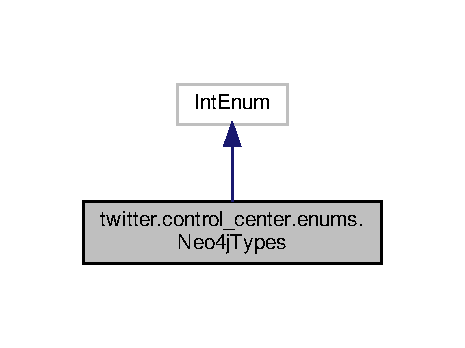
\includegraphics[width=223pt]{dd/d6e/classtwitter_1_1control__center_1_1enums_1_1Neo4jTypes__inherit__graph}
\end{center}
\end{figure}


Collaboration diagram for twitter.\+control\+\_\+center.\+enums.\+Neo4j\+Types\+:\nopagebreak
\begin{figure}[H]
\begin{center}
\leavevmode
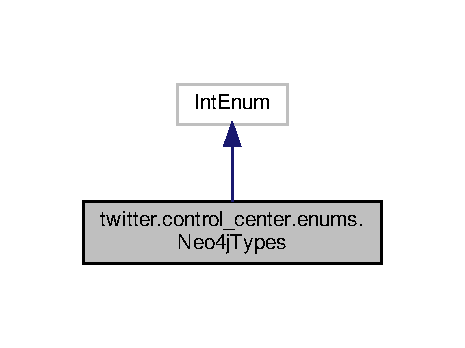
\includegraphics[width=223pt]{da/d1d/classtwitter_1_1control__center_1_1enums_1_1Neo4jTypes__coll__graph}
\end{center}
\end{figure}
\subsection*{Static Public Attributes}
\begin{DoxyCompactItemize}
\item 
\mbox{\Hypertarget{classtwitter_1_1control__center_1_1enums_1_1Neo4jTypes_ae3c56fb299eefc1481a2fe63cfdaa5e5}\label{classtwitter_1_1control__center_1_1enums_1_1Neo4jTypes_ae3c56fb299eefc1481a2fe63cfdaa5e5}} 
int {\bfseries C\+R\+E\+A\+T\+E\+\_\+\+B\+OT} = 1
\item 
\mbox{\Hypertarget{classtwitter_1_1control__center_1_1enums_1_1Neo4jTypes_a85b26cfbccbc0a85c141db505dad2b7d}\label{classtwitter_1_1control__center_1_1enums_1_1Neo4jTypes_a85b26cfbccbc0a85c141db505dad2b7d}} 
int {\bfseries C\+R\+E\+A\+T\+E\+\_\+\+U\+S\+ER} = 2
\item 
\mbox{\Hypertarget{classtwitter_1_1control__center_1_1enums_1_1Neo4jTypes_a6db78d0679448864cb2de85f154f66ff}\label{classtwitter_1_1control__center_1_1enums_1_1Neo4jTypes_a6db78d0679448864cb2de85f154f66ff}} 
int {\bfseries C\+R\+E\+A\+T\+E\+\_\+\+R\+E\+L\+A\+T\+I\+O\+N\+\_\+\+B\+O\+T\+\_\+\+U\+S\+ER} = 3
\item 
\mbox{\Hypertarget{classtwitter_1_1control__center_1_1enums_1_1Neo4jTypes_a380457ade6274f49db2b4cfb7d47370e}\label{classtwitter_1_1control__center_1_1enums_1_1Neo4jTypes_a380457ade6274f49db2b4cfb7d47370e}} 
int {\bfseries S\+E\+A\+R\+C\+H\+\_\+\+U\+S\+ER} = 4
\item 
\mbox{\Hypertarget{classtwitter_1_1control__center_1_1enums_1_1Neo4jTypes_a5f49d6ff2bf0d62e4d95d5dbc1af44ff}\label{classtwitter_1_1control__center_1_1enums_1_1Neo4jTypes_a5f49d6ff2bf0d62e4d95d5dbc1af44ff}} 
int {\bfseries U\+P\+D\+A\+T\+E\+\_\+\+U\+S\+ER} = 5
\item 
\mbox{\Hypertarget{classtwitter_1_1control__center_1_1enums_1_1Neo4jTypes_a67e0a96c5d0c6c8c0f66f7d89924ab3b}\label{classtwitter_1_1control__center_1_1enums_1_1Neo4jTypes_a67e0a96c5d0c6c8c0f66f7d89924ab3b}} 
int {\bfseries S\+E\+A\+R\+C\+H\+\_\+\+B\+OT} = 6
\item 
\mbox{\Hypertarget{classtwitter_1_1control__center_1_1enums_1_1Neo4jTypes_ad43693ab8b4f252b7eeccc9c09753593}\label{classtwitter_1_1control__center_1_1enums_1_1Neo4jTypes_ad43693ab8b4f252b7eeccc9c09753593}} 
int {\bfseries U\+P\+D\+A\+T\+E\+\_\+\+B\+OT} = 7
\item 
\mbox{\Hypertarget{classtwitter_1_1control__center_1_1enums_1_1Neo4jTypes_aba6f55ec115736865fe4fed5f20381bb}\label{classtwitter_1_1control__center_1_1enums_1_1Neo4jTypes_aba6f55ec115736865fe4fed5f20381bb}} 
int {\bfseries C\+R\+E\+A\+T\+E\+\_\+\+R\+E\+L\+A\+T\+I\+O\+N\+\_\+\+U\+S\+E\+R\+\_\+\+U\+S\+ER} = 8
\item 
\mbox{\Hypertarget{classtwitter_1_1control__center_1_1enums_1_1Neo4jTypes_ae2db8b3836f9d22d972c1687e3e589b0}\label{classtwitter_1_1control__center_1_1enums_1_1Neo4jTypes_ae2db8b3836f9d22d972c1687e3e589b0}} 
int {\bfseries C\+R\+E\+A\+T\+E\+\_\+\+R\+E\+L\+A\+T\+I\+O\+N\+\_\+\+B\+O\+T\+\_\+\+B\+OT} = 9
\end{DoxyCompactItemize}


The documentation for this class was generated from the following file\+:\begin{DoxyCompactItemize}
\item 
control\+\_\+center/enums.\+py\end{DoxyCompactItemize}

\hypertarget{classtwitter_1_1control__center_1_1PDP_1_1PDP}{}\section{twitter.\+control\+\_\+center.\+P\+D\+P.\+P\+DP Class Reference}
\label{classtwitter_1_1control__center_1_1PDP_1_1PDP}\index{twitter.\+control\+\_\+center.\+P\+D\+P.\+P\+DP@{twitter.\+control\+\_\+center.\+P\+D\+P.\+P\+DP}}
\subsection*{Public Member Functions}
\begin{DoxyCompactItemize}
\item 
def \hyperlink{classtwitter_1_1control__center_1_1PDP_1_1PDP_adf406e4b2ad47c65c563ccc7eccaf871}{\+\_\+\+\_\+init\+\_\+\+\_\+} (self)
\item 
\mbox{\Hypertarget{classtwitter_1_1control__center_1_1PDP_1_1PDP_af72d3a9d5544d71cf6d96369e79d0d37}\label{classtwitter_1_1control__center_1_1PDP_1_1PDP_af72d3a9d5544d71cf6d96369e79d0d37}} 
def {\bfseries receive\+\_\+request} (self, data)
\item 
def \hyperlink{classtwitter_1_1control__center_1_1PDP_1_1PDP_ad40264a760a1bdcb7563cb71955bb7f9}{evaluate} (self, msg)
\item 
\mbox{\Hypertarget{classtwitter_1_1control__center_1_1PDP_1_1PDP_ae0c0a77717da7489004c0b34b9fec771}\label{classtwitter_1_1control__center_1_1PDP_1_1PDP_ae0c0a77717da7489004c0b34b9fec771}} 
def {\bfseries send\+\_\+response} (self, msg)
\item 
def \hyperlink{classtwitter_1_1control__center_1_1PDP_1_1PDP_a5ac3bf5edb6f1913f09aecf0fe1ccc7f}{get\+\_\+first\+\_\+time\+\_\+list} (self)
\item 
def \hyperlink{classtwitter_1_1control__center_1_1PDP_1_1PDP_af6e05300883ddb19bcd9c6047e000ec1}{analyze\+\_\+tweet\+\_\+like} (self, data)
\item 
def \hyperlink{classtwitter_1_1control__center_1_1PDP_1_1PDP_ae173efc2c97b103ad0fbb0484c27835a}{analyze\+\_\+tweet\+\_\+retweet} (self, data)
\item 
def \hyperlink{classtwitter_1_1control__center_1_1PDP_1_1PDP_acbac2033b2853b89b3ee19ed040586e8}{analyze\+\_\+tweet\+\_\+reply} (self, data)
\item 
def \hyperlink{classtwitter_1_1control__center_1_1PDP_1_1PDP_ab9d69b04d93fc8b6fead61fd98991c22}{analyze\+\_\+follow\+\_\+user} (self, data)
\item 
\mbox{\Hypertarget{classtwitter_1_1control__center_1_1PDP_1_1PDP_ac3d2ce5166ecab928b14d231b322523f}\label{classtwitter_1_1control__center_1_1PDP_1_1PDP_ac3d2ce5166ecab928b14d231b322523f}} 
def {\bfseries close} (self)
\end{DoxyCompactItemize}
\subsection*{Public Attributes}
\begin{DoxyCompactItemize}
\item 
\mbox{\Hypertarget{classtwitter_1_1control__center_1_1PDP_1_1PDP_ac625eb8534bd8073613e9cccb21f1999}\label{classtwitter_1_1control__center_1_1PDP_1_1PDP_ac625eb8534bd8073613e9cccb21f1999}} 
{\bfseries mongo}
\item 
\mbox{\Hypertarget{classtwitter_1_1control__center_1_1PDP_1_1PDP_aba6c617ea663cbe89a36c4a879f0dda1}\label{classtwitter_1_1control__center_1_1PDP_1_1PDP_aba6c617ea663cbe89a36c4a879f0dda1}} 
{\bfseries neo4j}
\item 
\mbox{\Hypertarget{classtwitter_1_1control__center_1_1PDP_1_1PDP_afa535f42bb7f0e2e73f7acae08723756}\label{classtwitter_1_1control__center_1_1PDP_1_1PDP_afa535f42bb7f0e2e73f7acae08723756}} 
{\bfseries postgres}
\end{DoxyCompactItemize}


\subsection{Constructor \& Destructor Documentation}
\mbox{\Hypertarget{classtwitter_1_1control__center_1_1PDP_1_1PDP_adf406e4b2ad47c65c563ccc7eccaf871}\label{classtwitter_1_1control__center_1_1PDP_1_1PDP_adf406e4b2ad47c65c563ccc7eccaf871}} 
\index{twitter\+::control\+\_\+center\+::\+P\+D\+P\+::\+P\+DP@{twitter\+::control\+\_\+center\+::\+P\+D\+P\+::\+P\+DP}!\+\_\+\+\_\+init\+\_\+\+\_\+@{\+\_\+\+\_\+init\+\_\+\+\_\+}}
\index{\+\_\+\+\_\+init\+\_\+\+\_\+@{\+\_\+\+\_\+init\+\_\+\+\_\+}!twitter\+::control\+\_\+center\+::\+P\+D\+P\+::\+P\+DP@{twitter\+::control\+\_\+center\+::\+P\+D\+P\+::\+P\+DP}}
\subsubsection{\texorpdfstring{\+\_\+\+\_\+init\+\_\+\+\_\+()}{\_\_init\_\_()}}
{\footnotesize\ttfamily def twitter.\+control\+\_\+center.\+P\+D\+P.\+P\+D\+P.\+\_\+\+\_\+init\+\_\+\+\_\+ (\begin{DoxyParamCaption}\item[{}]{self }\end{DoxyParamCaption})}

\begin{DoxyVerb}Here starts the connections with the other DB wrappers
\end{DoxyVerb}
 

\subsection{Member Function Documentation}
\mbox{\Hypertarget{classtwitter_1_1control__center_1_1PDP_1_1PDP_ab9d69b04d93fc8b6fead61fd98991c22}\label{classtwitter_1_1control__center_1_1PDP_1_1PDP_ab9d69b04d93fc8b6fead61fd98991c22}} 
\index{twitter\+::control\+\_\+center\+::\+P\+D\+P\+::\+P\+DP@{twitter\+::control\+\_\+center\+::\+P\+D\+P\+::\+P\+DP}!analyze\+\_\+follow\+\_\+user@{analyze\+\_\+follow\+\_\+user}}
\index{analyze\+\_\+follow\+\_\+user@{analyze\+\_\+follow\+\_\+user}!twitter\+::control\+\_\+center\+::\+P\+D\+P\+::\+P\+DP@{twitter\+::control\+\_\+center\+::\+P\+D\+P\+::\+P\+DP}}
\subsubsection{\texorpdfstring{analyze\+\_\+follow\+\_\+user()}{analyze\_follow\_user()}}
{\footnotesize\ttfamily def twitter.\+control\+\_\+center.\+P\+D\+P.\+P\+D\+P.\+analyze\+\_\+follow\+\_\+user (\begin{DoxyParamCaption}\item[{}]{self,  }\item[{}]{data }\end{DoxyParamCaption})}

\begin{DoxyVerb}Algorithm to analyse if a bot should follow
Takes the current statistics and turns them into a real value

@param: data - dictionary containing the data of the bot and the tweet it wants to like
@returns: float that will then be compared to the threshold previously defined
\end{DoxyVerb}
 \mbox{\Hypertarget{classtwitter_1_1control__center_1_1PDP_1_1PDP_af6e05300883ddb19bcd9c6047e000ec1}\label{classtwitter_1_1control__center_1_1PDP_1_1PDP_af6e05300883ddb19bcd9c6047e000ec1}} 
\index{twitter\+::control\+\_\+center\+::\+P\+D\+P\+::\+P\+DP@{twitter\+::control\+\_\+center\+::\+P\+D\+P\+::\+P\+DP}!analyze\+\_\+tweet\+\_\+like@{analyze\+\_\+tweet\+\_\+like}}
\index{analyze\+\_\+tweet\+\_\+like@{analyze\+\_\+tweet\+\_\+like}!twitter\+::control\+\_\+center\+::\+P\+D\+P\+::\+P\+DP@{twitter\+::control\+\_\+center\+::\+P\+D\+P\+::\+P\+DP}}
\subsubsection{\texorpdfstring{analyze\+\_\+tweet\+\_\+like()}{analyze\_tweet\_like()}}
{\footnotesize\ttfamily def twitter.\+control\+\_\+center.\+P\+D\+P.\+P\+D\+P.\+analyze\+\_\+tweet\+\_\+like (\begin{DoxyParamCaption}\item[{}]{self,  }\item[{}]{data }\end{DoxyParamCaption})}

\begin{DoxyVerb}Algorithm to analyse if a bot should like a Tweet
Takes the current statistics and turns them into a real value

@param: data - dictionary containing the data of the bot and the tweet it wants to like
@returns: float that will then be compared to the threshold previously defined
\end{DoxyVerb}
 \mbox{\Hypertarget{classtwitter_1_1control__center_1_1PDP_1_1PDP_acbac2033b2853b89b3ee19ed040586e8}\label{classtwitter_1_1control__center_1_1PDP_1_1PDP_acbac2033b2853b89b3ee19ed040586e8}} 
\index{twitter\+::control\+\_\+center\+::\+P\+D\+P\+::\+P\+DP@{twitter\+::control\+\_\+center\+::\+P\+D\+P\+::\+P\+DP}!analyze\+\_\+tweet\+\_\+reply@{analyze\+\_\+tweet\+\_\+reply}}
\index{analyze\+\_\+tweet\+\_\+reply@{analyze\+\_\+tweet\+\_\+reply}!twitter\+::control\+\_\+center\+::\+P\+D\+P\+::\+P\+DP@{twitter\+::control\+\_\+center\+::\+P\+D\+P\+::\+P\+DP}}
\subsubsection{\texorpdfstring{analyze\+\_\+tweet\+\_\+reply()}{analyze\_tweet\_reply()}}
{\footnotesize\ttfamily def twitter.\+control\+\_\+center.\+P\+D\+P.\+P\+D\+P.\+analyze\+\_\+tweet\+\_\+reply (\begin{DoxyParamCaption}\item[{}]{self,  }\item[{}]{data }\end{DoxyParamCaption})}

\begin{DoxyVerb}Algorithm to analyse if a bot should reply
Takes the current statistics and turns them into a real value

@param: data - dictionary containing the data of the bot and the tweet it wants to like
@returns: float that will then be compared to the threshold previously defined
\end{DoxyVerb}
 \mbox{\Hypertarget{classtwitter_1_1control__center_1_1PDP_1_1PDP_ae173efc2c97b103ad0fbb0484c27835a}\label{classtwitter_1_1control__center_1_1PDP_1_1PDP_ae173efc2c97b103ad0fbb0484c27835a}} 
\index{twitter\+::control\+\_\+center\+::\+P\+D\+P\+::\+P\+DP@{twitter\+::control\+\_\+center\+::\+P\+D\+P\+::\+P\+DP}!analyze\+\_\+tweet\+\_\+retweet@{analyze\+\_\+tweet\+\_\+retweet}}
\index{analyze\+\_\+tweet\+\_\+retweet@{analyze\+\_\+tweet\+\_\+retweet}!twitter\+::control\+\_\+center\+::\+P\+D\+P\+::\+P\+DP@{twitter\+::control\+\_\+center\+::\+P\+D\+P\+::\+P\+DP}}
\subsubsection{\texorpdfstring{analyze\+\_\+tweet\+\_\+retweet()}{analyze\_tweet\_retweet()}}
{\footnotesize\ttfamily def twitter.\+control\+\_\+center.\+P\+D\+P.\+P\+D\+P.\+analyze\+\_\+tweet\+\_\+retweet (\begin{DoxyParamCaption}\item[{}]{self,  }\item[{}]{data }\end{DoxyParamCaption})}

\begin{DoxyVerb}Algorithm to analyse if a bot should retweet a Tweet
Takes the current statistics and turns them into a real value

@param: data - dictionary containing the data of the bot and the tweet it wants to like
@returns: float that will then be compared to the threshold previously defined
\end{DoxyVerb}
 \mbox{\Hypertarget{classtwitter_1_1control__center_1_1PDP_1_1PDP_ad40264a760a1bdcb7563cb71955bb7f9}\label{classtwitter_1_1control__center_1_1PDP_1_1PDP_ad40264a760a1bdcb7563cb71955bb7f9}} 
\index{twitter\+::control\+\_\+center\+::\+P\+D\+P\+::\+P\+DP@{twitter\+::control\+\_\+center\+::\+P\+D\+P\+::\+P\+DP}!evaluate@{evaluate}}
\index{evaluate@{evaluate}!twitter\+::control\+\_\+center\+::\+P\+D\+P\+::\+P\+DP@{twitter\+::control\+\_\+center\+::\+P\+D\+P\+::\+P\+DP}}
\subsubsection{\texorpdfstring{evaluate()}{evaluate()}}
{\footnotesize\ttfamily def twitter.\+control\+\_\+center.\+P\+D\+P.\+P\+D\+P.\+evaluate (\begin{DoxyParamCaption}\item[{}]{self,  }\item[{}]{msg }\end{DoxyParamCaption})}

\begin{DoxyVerb}Workflow of this function:
    1. pre-processing of request (filter, prepare db request, etc)
    2. request to DB
    3. get request from DB
    4. post-processing of response (clean response from db, etc)
    5. DECIDE (PERMIT, DENY)

@param msg : dict
    Dictionary with necessary fields to perform the query.
    Something of this form: { "type" : action, data }

@return response:
    A response with either "DENY" or "PERMIT"
\end{DoxyVerb}
 \mbox{\Hypertarget{classtwitter_1_1control__center_1_1PDP_1_1PDP_a5ac3bf5edb6f1913f09aecf0fe1ccc7f}\label{classtwitter_1_1control__center_1_1PDP_1_1PDP_a5ac3bf5edb6f1913f09aecf0fe1ccc7f}} 
\index{twitter\+::control\+\_\+center\+::\+P\+D\+P\+::\+P\+DP@{twitter\+::control\+\_\+center\+::\+P\+D\+P\+::\+P\+DP}!get\+\_\+first\+\_\+time\+\_\+list@{get\+\_\+first\+\_\+time\+\_\+list}}
\index{get\+\_\+first\+\_\+time\+\_\+list@{get\+\_\+first\+\_\+time\+\_\+list}!twitter\+::control\+\_\+center\+::\+P\+D\+P\+::\+P\+DP@{twitter\+::control\+\_\+center\+::\+P\+D\+P\+::\+P\+DP}}
\subsubsection{\texorpdfstring{get\+\_\+first\+\_\+time\+\_\+list()}{get\_first\_time\_list()}}
{\footnotesize\ttfamily def twitter.\+control\+\_\+center.\+P\+D\+P.\+P\+D\+P.\+get\+\_\+first\+\_\+time\+\_\+list (\begin{DoxyParamCaption}\item[{}]{self }\end{DoxyParamCaption})}

\begin{DoxyVerb}When a bot connects for the first time to Twitter, he'll have to start following people This is the old way:
having a set list of possible users and the bot will follow a random group from those followers In future
iterations we may alter this so that there are possible branches a bot could start with: politics,
football fan, etc., each branch with a list of possible users to follow

@return: List of users the bot will start following
\end{DoxyVerb}
 

The documentation for this class was generated from the following file\+:\begin{DoxyCompactItemize}
\item 
control\+\_\+center/P\+D\+P.\+py\end{DoxyCompactItemize}

\hypertarget{classtwitter_1_1control__center_1_1PEP_1_1PEP}{}\section{twitter.\+control\+\_\+center.\+P\+E\+P.\+P\+EP Class Reference}
\label{classtwitter_1_1control__center_1_1PEP_1_1PEP}\index{twitter.\+control\+\_\+center.\+P\+E\+P.\+P\+EP@{twitter.\+control\+\_\+center.\+P\+E\+P.\+P\+EP}}
\subsection*{Public Member Functions}
\begin{DoxyCompactItemize}
\item 
def \hyperlink{classtwitter_1_1control__center_1_1PEP_1_1PEP_a39f16437e59b0aba7094713042e0a6a6}{\+\_\+\+\_\+init\+\_\+\+\_\+} (self)
\item 
def \hyperlink{classtwitter_1_1control__center_1_1PEP_1_1PEP_af13289593fcd0c6d2e945b9431642120}{first\+\_\+time\+\_\+policy} (self)
\item 
def \hyperlink{classtwitter_1_1control__center_1_1PEP_1_1PEP_a77d6cfa9b9fed7164b8c370b7147922f}{receive\+\_\+message} (self, msg)
\item 
def \hyperlink{classtwitter_1_1control__center_1_1PEP_1_1PEP_ad3d661b529e2bd004eda5e3746dab298}{enforce} (self, data)
\end{DoxyCompactItemize}
\subsection*{Public Attributes}
\begin{DoxyCompactItemize}
\item 
\mbox{\Hypertarget{classtwitter_1_1control__center_1_1PEP_1_1PEP_a240eab8688830086e20637c393743af7}\label{classtwitter_1_1control__center_1_1PEP_1_1PEP_a240eab8688830086e20637c393743af7}} 
{\bfseries pdp}
\end{DoxyCompactItemize}


\subsection{Detailed Description}
\begin{DoxyVerb}Policy Enforcement Point
Class who connects to the PDP - Policy Decision Point and forwards its result to the bot
\end{DoxyVerb}
 

\subsection{Constructor \& Destructor Documentation}
\mbox{\Hypertarget{classtwitter_1_1control__center_1_1PEP_1_1PEP_a39f16437e59b0aba7094713042e0a6a6}\label{classtwitter_1_1control__center_1_1PEP_1_1PEP_a39f16437e59b0aba7094713042e0a6a6}} 
\index{twitter\+::control\+\_\+center\+::\+P\+E\+P\+::\+P\+EP@{twitter\+::control\+\_\+center\+::\+P\+E\+P\+::\+P\+EP}!\+\_\+\+\_\+init\+\_\+\+\_\+@{\+\_\+\+\_\+init\+\_\+\+\_\+}}
\index{\+\_\+\+\_\+init\+\_\+\+\_\+@{\+\_\+\+\_\+init\+\_\+\+\_\+}!twitter\+::control\+\_\+center\+::\+P\+E\+P\+::\+P\+EP@{twitter\+::control\+\_\+center\+::\+P\+E\+P\+::\+P\+EP}}
\subsubsection{\texorpdfstring{\+\_\+\+\_\+init\+\_\+\+\_\+()}{\_\_init\_\_()}}
{\footnotesize\ttfamily def twitter.\+control\+\_\+center.\+P\+E\+P.\+P\+E\+P.\+\_\+\+\_\+init\+\_\+\+\_\+ (\begin{DoxyParamCaption}\item[{}]{self }\end{DoxyParamCaption})}

\begin{DoxyVerb}It may need the PDP to be passed as argument, but for now it's creating a new object every time
\end{DoxyVerb}
 

\subsection{Member Function Documentation}
\mbox{\Hypertarget{classtwitter_1_1control__center_1_1PEP_1_1PEP_ad3d661b529e2bd004eda5e3746dab298}\label{classtwitter_1_1control__center_1_1PEP_1_1PEP_ad3d661b529e2bd004eda5e3746dab298}} 
\index{twitter\+::control\+\_\+center\+::\+P\+E\+P\+::\+P\+EP@{twitter\+::control\+\_\+center\+::\+P\+E\+P\+::\+P\+EP}!enforce@{enforce}}
\index{enforce@{enforce}!twitter\+::control\+\_\+center\+::\+P\+E\+P\+::\+P\+EP@{twitter\+::control\+\_\+center\+::\+P\+E\+P\+::\+P\+EP}}
\subsubsection{\texorpdfstring{enforce()}{enforce()}}
{\footnotesize\ttfamily def twitter.\+control\+\_\+center.\+P\+E\+P.\+P\+E\+P.\+enforce (\begin{DoxyParamCaption}\item[{}]{self,  }\item[{}]{data }\end{DoxyParamCaption})}

\begin{DoxyVerb}The enforce method will simply turn the response into a boolean value the bot can understand

@param data: a dictionaru containing the result of the PDP's logic

@return Boolean permitting/denying the behaviour
\end{DoxyVerb}
 \mbox{\Hypertarget{classtwitter_1_1control__center_1_1PEP_1_1PEP_af13289593fcd0c6d2e945b9431642120}\label{classtwitter_1_1control__center_1_1PEP_1_1PEP_af13289593fcd0c6d2e945b9431642120}} 
\index{twitter\+::control\+\_\+center\+::\+P\+E\+P\+::\+P\+EP@{twitter\+::control\+\_\+center\+::\+P\+E\+P\+::\+P\+EP}!first\+\_\+time\+\_\+policy@{first\+\_\+time\+\_\+policy}}
\index{first\+\_\+time\+\_\+policy@{first\+\_\+time\+\_\+policy}!twitter\+::control\+\_\+center\+::\+P\+E\+P\+::\+P\+EP@{twitter\+::control\+\_\+center\+::\+P\+E\+P\+::\+P\+EP}}
\subsubsection{\texorpdfstring{first\+\_\+time\+\_\+policy()}{first\_time\_policy()}}
{\footnotesize\ttfamily def twitter.\+control\+\_\+center.\+P\+E\+P.\+P\+E\+P.\+first\+\_\+time\+\_\+policy (\begin{DoxyParamCaption}\item[{}]{self }\end{DoxyParamCaption})}

\begin{DoxyVerb}If a bot has just arrived to twitter, it must be handed a list of initial users for it to follow
The list is decided by the PDP, and there's no need for extra params, since it's pretty much chosen at random, for now
\end{DoxyVerb}
 \mbox{\Hypertarget{classtwitter_1_1control__center_1_1PEP_1_1PEP_a77d6cfa9b9fed7164b8c370b7147922f}\label{classtwitter_1_1control__center_1_1PEP_1_1PEP_a77d6cfa9b9fed7164b8c370b7147922f}} 
\index{twitter\+::control\+\_\+center\+::\+P\+E\+P\+::\+P\+EP@{twitter\+::control\+\_\+center\+::\+P\+E\+P\+::\+P\+EP}!receive\+\_\+message@{receive\+\_\+message}}
\index{receive\+\_\+message@{receive\+\_\+message}!twitter\+::control\+\_\+center\+::\+P\+E\+P\+::\+P\+EP@{twitter\+::control\+\_\+center\+::\+P\+E\+P\+::\+P\+EP}}
\subsubsection{\texorpdfstring{receive\+\_\+message()}{receive\_message()}}
{\footnotesize\ttfamily def twitter.\+control\+\_\+center.\+P\+E\+P.\+P\+E\+P.\+receive\+\_\+message (\begin{DoxyParamCaption}\item[{}]{self,  }\item[{}]{msg }\end{DoxyParamCaption})}

\begin{DoxyVerb}The receive message applies to when a request comes to this point, for now, the PEP will start by forwarding that message
After receiving the response from the PDP object, it will enforce a behaviour based on the response

@param msg - a dictionary containing the message to be passed on
\end{DoxyVerb}
 

The documentation for this class was generated from the following file\+:\begin{DoxyCompactItemize}
\item 
control\+\_\+center/P\+E\+P.\+py\end{DoxyCompactItemize}

\hypertarget{classtwitter_1_1control__center_1_1enums_1_1PoliciesTypes}{}\section{twitter.\+control\+\_\+center.\+enums.\+Policies\+Types Class Reference}
\label{classtwitter_1_1control__center_1_1enums_1_1PoliciesTypes}\index{twitter.\+control\+\_\+center.\+enums.\+Policies\+Types@{twitter.\+control\+\_\+center.\+enums.\+Policies\+Types}}


Inheritance diagram for twitter.\+control\+\_\+center.\+enums.\+Policies\+Types\+:\nopagebreak
\begin{figure}[H]
\begin{center}
\leavevmode
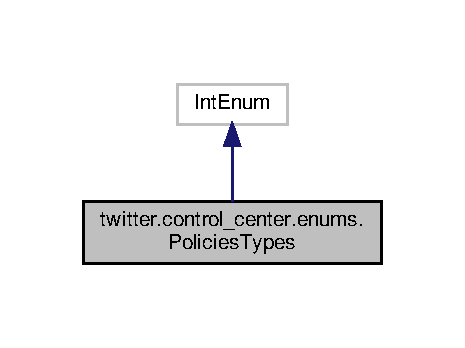
\includegraphics[width=223pt]{d5/d7f/classtwitter_1_1control__center_1_1enums_1_1PoliciesTypes__inherit__graph}
\end{center}
\end{figure}


Collaboration diagram for twitter.\+control\+\_\+center.\+enums.\+Policies\+Types\+:\nopagebreak
\begin{figure}[H]
\begin{center}
\leavevmode
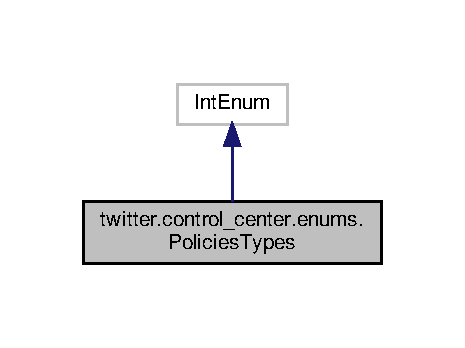
\includegraphics[width=223pt]{d4/d25/classtwitter_1_1control__center_1_1enums_1_1PoliciesTypes__coll__graph}
\end{center}
\end{figure}
\subsection*{Static Public Attributes}
\begin{DoxyCompactItemize}
\item 
\mbox{\Hypertarget{classtwitter_1_1control__center_1_1enums_1_1PoliciesTypes_a26ce4fe53c91441a04f58fa33d923883}\label{classtwitter_1_1control__center_1_1enums_1_1PoliciesTypes_a26ce4fe53c91441a04f58fa33d923883}} 
int {\bfseries R\+E\+Q\+U\+E\+S\+T\+\_\+\+T\+W\+E\+E\+T\+\_\+\+L\+I\+KE} = 1
\item 
\mbox{\Hypertarget{classtwitter_1_1control__center_1_1enums_1_1PoliciesTypes_a496393fa4829947c2576faad82518712}\label{classtwitter_1_1control__center_1_1enums_1_1PoliciesTypes_a496393fa4829947c2576faad82518712}} 
int {\bfseries R\+E\+Q\+U\+E\+S\+T\+\_\+\+T\+W\+E\+E\+T\+\_\+\+R\+E\+T\+W\+E\+ET} = 2
\item 
\mbox{\Hypertarget{classtwitter_1_1control__center_1_1enums_1_1PoliciesTypes_a3a5e4c87466c7021797f0b0bea368431}\label{classtwitter_1_1control__center_1_1enums_1_1PoliciesTypes_a3a5e4c87466c7021797f0b0bea368431}} 
int {\bfseries R\+E\+Q\+U\+E\+S\+T\+\_\+\+T\+W\+E\+E\+T\+\_\+\+R\+E\+P\+LY} = 3
\item 
\mbox{\Hypertarget{classtwitter_1_1control__center_1_1enums_1_1PoliciesTypes_ad632b0f87c850d92691982ababaaaec8}\label{classtwitter_1_1control__center_1_1enums_1_1PoliciesTypes_ad632b0f87c850d92691982ababaaaec8}} 
int {\bfseries R\+E\+Q\+U\+E\+S\+T\+\_\+\+F\+O\+L\+L\+O\+W\+\_\+\+U\+S\+ER} = 4
\item 
\mbox{\Hypertarget{classtwitter_1_1control__center_1_1enums_1_1PoliciesTypes_a9adf39df52f67f73d6c25e4d28cbb0bb}\label{classtwitter_1_1control__center_1_1enums_1_1PoliciesTypes_a9adf39df52f67f73d6c25e4d28cbb0bb}} 
int {\bfseries F\+I\+R\+S\+T\+\_\+\+T\+I\+ME} = 5
\end{DoxyCompactItemize}


The documentation for this class was generated from the following file\+:\begin{DoxyCompactItemize}
\item 
control\+\_\+center/enums.\+py\end{DoxyCompactItemize}

\hypertarget{classtwitter_1_1wrappers_1_1postgresql__wrapper_1_1PostgresAPI}{}\section{twitter.\+wrappers.\+postgresql\+\_\+wrapper.\+Postgres\+A\+PI Class Reference}
\label{classtwitter_1_1wrappers_1_1postgresql__wrapper_1_1PostgresAPI}\index{twitter.\+wrappers.\+postgresql\+\_\+wrapper.\+Postgres\+A\+PI@{twitter.\+wrappers.\+postgresql\+\_\+wrapper.\+Postgres\+A\+PI}}
\subsection*{Public Member Functions}
\begin{DoxyCompactItemize}
\item 
\mbox{\Hypertarget{classtwitter_1_1wrappers_1_1postgresql__wrapper_1_1PostgresAPI_a18adcc26af89165719564d5f90d5baa2}\label{classtwitter_1_1wrappers_1_1postgresql__wrapper_1_1PostgresAPI_a18adcc26af89165719564d5f90d5baa2}} 
def {\bfseries \+\_\+\+\_\+init\+\_\+\+\_\+} (self)
\item 
def \hyperlink{classtwitter_1_1wrappers_1_1postgresql__wrapper_1_1PostgresAPI_a6b2b617a04ade9f12c63996210b2287b}{insert\+\_\+tweet} (self, data)
\item 
def \hyperlink{classtwitter_1_1wrappers_1_1postgresql__wrapper_1_1PostgresAPI_ae94da23c6824c6db14d62624eee98325}{insert\+\_\+user} (self, data)
\item 
def \hyperlink{classtwitter_1_1wrappers_1_1postgresql__wrapper_1_1PostgresAPI_a772c1a47184e165cfe9958c78a97a146}{search\+\_\+tweet} (self, params=None)
\item 
def \hyperlink{classtwitter_1_1wrappers_1_1postgresql__wrapper_1_1PostgresAPI_a84fa6c90c91f88a68284fba6812b043f}{search\+\_\+user} (self, params=None)
\item 
def \hyperlink{classtwitter_1_1wrappers_1_1postgresql__wrapper_1_1PostgresAPI_a85bdfe473c1bd0bd29e11c059e7cb3dc}{search\+\_\+logs} (self, params=None, limit=None)
\item 
def \hyperlink{classtwitter_1_1wrappers_1_1postgresql__wrapper_1_1PostgresAPI_aeac23865a14e4f32e90cb7daa4a03e2b}{search\+\_\+policies} (self, params=None, limit=None)
\item 
def \hyperlink{classtwitter_1_1wrappers_1_1postgresql__wrapper_1_1PostgresAPI_ae0a6d7340ffc3d83829308940a296393}{insert\+\_\+log} (self, data)
\item 
def \hyperlink{classtwitter_1_1wrappers_1_1postgresql__wrapper_1_1PostgresAPI_a97ea1442f99c7a75f996024dd3e3da8c}{insert\+\_\+policy} (self, data)
\item 
def \hyperlink{classtwitter_1_1wrappers_1_1postgresql__wrapper_1_1PostgresAPI_a93b51196b75f21a7061a027a0b530bf0}{delete\+\_\+policy} (self, policy\+\_\+id)
\item 
def \hyperlink{classtwitter_1_1wrappers_1_1postgresql__wrapper_1_1PostgresAPI_aa32ee622eb02190f09ec38919123bbb5}{update\+\_\+policy} (self, policy\+\_\+id, params)
\end{DoxyCompactItemize}
\subsection*{Public Attributes}
\begin{DoxyCompactItemize}
\item 
\mbox{\Hypertarget{classtwitter_1_1wrappers_1_1postgresql__wrapper_1_1PostgresAPI_afadde44f92f712763ef7d0aeaea2ef0f}\label{classtwitter_1_1wrappers_1_1postgresql__wrapper_1_1PostgresAPI_afadde44f92f712763ef7d0aeaea2ef0f}} 
{\bfseries conn}
\item 
\mbox{\Hypertarget{classtwitter_1_1wrappers_1_1postgresql__wrapper_1_1PostgresAPI_aed05e237c349e83bbcb76eccaf4f56df}\label{classtwitter_1_1wrappers_1_1postgresql__wrapper_1_1PostgresAPI_aed05e237c349e83bbcb76eccaf4f56df}} 
{\bfseries api\+\_\+types}
\item 
\mbox{\Hypertarget{classtwitter_1_1wrappers_1_1postgresql__wrapper_1_1PostgresAPI_ad5c56fa3b0421230409f1a4268fcfa26}\label{classtwitter_1_1wrappers_1_1postgresql__wrapper_1_1PostgresAPI_ad5c56fa3b0421230409f1a4268fcfa26}} 
{\bfseries filters}
\end{DoxyCompactItemize}


\subsection{Detailed Description}
\begin{DoxyVerb}PostgreSQL

Encompasses methods used for all API and PDP interactions with our PostgreSQL DB.
\end{DoxyVerb}
 

\subsection{Member Function Documentation}
\mbox{\Hypertarget{classtwitter_1_1wrappers_1_1postgresql__wrapper_1_1PostgresAPI_a93b51196b75f21a7061a027a0b530bf0}\label{classtwitter_1_1wrappers_1_1postgresql__wrapper_1_1PostgresAPI_a93b51196b75f21a7061a027a0b530bf0}} 
\index{twitter\+::wrappers\+::postgresql\+\_\+wrapper\+::\+Postgres\+A\+PI@{twitter\+::wrappers\+::postgresql\+\_\+wrapper\+::\+Postgres\+A\+PI}!delete\+\_\+policy@{delete\+\_\+policy}}
\index{delete\+\_\+policy@{delete\+\_\+policy}!twitter\+::wrappers\+::postgresql\+\_\+wrapper\+::\+Postgres\+A\+PI@{twitter\+::wrappers\+::postgresql\+\_\+wrapper\+::\+Postgres\+A\+PI}}
\subsubsection{\texorpdfstring{delete\+\_\+policy()}{delete\_policy()}}
{\footnotesize\ttfamily def twitter.\+wrappers.\+postgresql\+\_\+wrapper.\+Postgres\+A\+P\+I.\+delete\+\_\+policy (\begin{DoxyParamCaption}\item[{}]{self,  }\item[{}]{policy\+\_\+id }\end{DoxyParamCaption})}

\begin{DoxyVerb}Deletes the policy with the given id

@param policy_id: The id of the policy we want to delete
@param limit: An optional parameter specifying the amount of logs to be retrieved

@return The query's result or error
\end{DoxyVerb}
 \mbox{\Hypertarget{classtwitter_1_1wrappers_1_1postgresql__wrapper_1_1PostgresAPI_ae0a6d7340ffc3d83829308940a296393}\label{classtwitter_1_1wrappers_1_1postgresql__wrapper_1_1PostgresAPI_ae0a6d7340ffc3d83829308940a296393}} 
\index{twitter\+::wrappers\+::postgresql\+\_\+wrapper\+::\+Postgres\+A\+PI@{twitter\+::wrappers\+::postgresql\+\_\+wrapper\+::\+Postgres\+A\+PI}!insert\+\_\+log@{insert\+\_\+log}}
\index{insert\+\_\+log@{insert\+\_\+log}!twitter\+::wrappers\+::postgresql\+\_\+wrapper\+::\+Postgres\+A\+PI@{twitter\+::wrappers\+::postgresql\+\_\+wrapper\+::\+Postgres\+A\+PI}}
\subsubsection{\texorpdfstring{insert\+\_\+log()}{insert\_log()}}
{\footnotesize\ttfamily def twitter.\+wrappers.\+postgresql\+\_\+wrapper.\+Postgres\+A\+P\+I.\+insert\+\_\+log (\begin{DoxyParamCaption}\item[{}]{self,  }\item[{}]{data }\end{DoxyParamCaption})}

\begin{DoxyVerb}Attempts to insert a new Log item into the database

@param data: The data of the item we want to insert. Should have
@return A success or failure message ({success: True/False ; error: None/Error})
\end{DoxyVerb}
 \mbox{\Hypertarget{classtwitter_1_1wrappers_1_1postgresql__wrapper_1_1PostgresAPI_a97ea1442f99c7a75f996024dd3e3da8c}\label{classtwitter_1_1wrappers_1_1postgresql__wrapper_1_1PostgresAPI_a97ea1442f99c7a75f996024dd3e3da8c}} 
\index{twitter\+::wrappers\+::postgresql\+\_\+wrapper\+::\+Postgres\+A\+PI@{twitter\+::wrappers\+::postgresql\+\_\+wrapper\+::\+Postgres\+A\+PI}!insert\+\_\+policy@{insert\+\_\+policy}}
\index{insert\+\_\+policy@{insert\+\_\+policy}!twitter\+::wrappers\+::postgresql\+\_\+wrapper\+::\+Postgres\+A\+PI@{twitter\+::wrappers\+::postgresql\+\_\+wrapper\+::\+Postgres\+A\+PI}}
\subsubsection{\texorpdfstring{insert\+\_\+policy()}{insert\_policy()}}
{\footnotesize\ttfamily def twitter.\+wrappers.\+postgresql\+\_\+wrapper.\+Postgres\+A\+P\+I.\+insert\+\_\+policy (\begin{DoxyParamCaption}\item[{}]{self,  }\item[{}]{data }\end{DoxyParamCaption})}

\begin{DoxyVerb}Attempts to insert a new Log item into the database

@param data: The data of the item we want to insert.
@return A success or failure message ({success: True/False ; error: None/Error})
\end{DoxyVerb}
 \mbox{\Hypertarget{classtwitter_1_1wrappers_1_1postgresql__wrapper_1_1PostgresAPI_a6b2b617a04ade9f12c63996210b2287b}\label{classtwitter_1_1wrappers_1_1postgresql__wrapper_1_1PostgresAPI_a6b2b617a04ade9f12c63996210b2287b}} 
\index{twitter\+::wrappers\+::postgresql\+\_\+wrapper\+::\+Postgres\+A\+PI@{twitter\+::wrappers\+::postgresql\+\_\+wrapper\+::\+Postgres\+A\+PI}!insert\+\_\+tweet@{insert\+\_\+tweet}}
\index{insert\+\_\+tweet@{insert\+\_\+tweet}!twitter\+::wrappers\+::postgresql\+\_\+wrapper\+::\+Postgres\+A\+PI@{twitter\+::wrappers\+::postgresql\+\_\+wrapper\+::\+Postgres\+A\+PI}}
\subsubsection{\texorpdfstring{insert\+\_\+tweet()}{insert\_tweet()}}
{\footnotesize\ttfamily def twitter.\+wrappers.\+postgresql\+\_\+wrapper.\+Postgres\+A\+P\+I.\+insert\+\_\+tweet (\begin{DoxyParamCaption}\item[{}]{self,  }\item[{}]{data }\end{DoxyParamCaption})}

\begin{DoxyVerb}Attempts to insert a new Tweet item into the database

@param data: The data of the item we want to insert. Should have - tweet_id, user_id, likes, retweets
@return A success or failure message ({success: True/False ; error: None/Error})
\end{DoxyVerb}
 \mbox{\Hypertarget{classtwitter_1_1wrappers_1_1postgresql__wrapper_1_1PostgresAPI_ae94da23c6824c6db14d62624eee98325}\label{classtwitter_1_1wrappers_1_1postgresql__wrapper_1_1PostgresAPI_ae94da23c6824c6db14d62624eee98325}} 
\index{twitter\+::wrappers\+::postgresql\+\_\+wrapper\+::\+Postgres\+A\+PI@{twitter\+::wrappers\+::postgresql\+\_\+wrapper\+::\+Postgres\+A\+PI}!insert\+\_\+user@{insert\+\_\+user}}
\index{insert\+\_\+user@{insert\+\_\+user}!twitter\+::wrappers\+::postgresql\+\_\+wrapper\+::\+Postgres\+A\+PI@{twitter\+::wrappers\+::postgresql\+\_\+wrapper\+::\+Postgres\+A\+PI}}
\subsubsection{\texorpdfstring{insert\+\_\+user()}{insert\_user()}}
{\footnotesize\ttfamily def twitter.\+wrappers.\+postgresql\+\_\+wrapper.\+Postgres\+A\+P\+I.\+insert\+\_\+user (\begin{DoxyParamCaption}\item[{}]{self,  }\item[{}]{data }\end{DoxyParamCaption})}

\begin{DoxyVerb}Attempts to insert a new User item into the database

@param data: The collection we want to insert the document into
@return A success or failure message ({success: True/False ; error: None/Error})
\end{DoxyVerb}
 \mbox{\Hypertarget{classtwitter_1_1wrappers_1_1postgresql__wrapper_1_1PostgresAPI_a85bdfe473c1bd0bd29e11c059e7cb3dc}\label{classtwitter_1_1wrappers_1_1postgresql__wrapper_1_1PostgresAPI_a85bdfe473c1bd0bd29e11c059e7cb3dc}} 
\index{twitter\+::wrappers\+::postgresql\+\_\+wrapper\+::\+Postgres\+A\+PI@{twitter\+::wrappers\+::postgresql\+\_\+wrapper\+::\+Postgres\+A\+PI}!search\+\_\+logs@{search\+\_\+logs}}
\index{search\+\_\+logs@{search\+\_\+logs}!twitter\+::wrappers\+::postgresql\+\_\+wrapper\+::\+Postgres\+A\+PI@{twitter\+::wrappers\+::postgresql\+\_\+wrapper\+::\+Postgres\+A\+PI}}
\subsubsection{\texorpdfstring{search\+\_\+logs()}{search\_logs()}}
{\footnotesize\ttfamily def twitter.\+wrappers.\+postgresql\+\_\+wrapper.\+Postgres\+A\+P\+I.\+search\+\_\+logs (\begin{DoxyParamCaption}\item[{}]{self,  }\item[{}]{params = {\ttfamily None},  }\item[{}]{limit = {\ttfamily None} }\end{DoxyParamCaption})}

\begin{DoxyVerb}Searches and returns all logs if no data is specified, or the specific logs matching the parameters. Can also
specify the amount of logs to be retrieved. Data retrieved is ordered by the most recent

@param params: The parameters we want to query. Right now only bot_id is supported
@param limit: An optional parameter specifying the amount of logs to be retrieved

@return The query's result or error
\end{DoxyVerb}
 \mbox{\Hypertarget{classtwitter_1_1wrappers_1_1postgresql__wrapper_1_1PostgresAPI_aeac23865a14e4f32e90cb7daa4a03e2b}\label{classtwitter_1_1wrappers_1_1postgresql__wrapper_1_1PostgresAPI_aeac23865a14e4f32e90cb7daa4a03e2b}} 
\index{twitter\+::wrappers\+::postgresql\+\_\+wrapper\+::\+Postgres\+A\+PI@{twitter\+::wrappers\+::postgresql\+\_\+wrapper\+::\+Postgres\+A\+PI}!search\+\_\+policies@{search\+\_\+policies}}
\index{search\+\_\+policies@{search\+\_\+policies}!twitter\+::wrappers\+::postgresql\+\_\+wrapper\+::\+Postgres\+A\+PI@{twitter\+::wrappers\+::postgresql\+\_\+wrapper\+::\+Postgres\+A\+PI}}
\subsubsection{\texorpdfstring{search\+\_\+policies()}{search\_policies()}}
{\footnotesize\ttfamily def twitter.\+wrappers.\+postgresql\+\_\+wrapper.\+Postgres\+A\+P\+I.\+search\+\_\+policies (\begin{DoxyParamCaption}\item[{}]{self,  }\item[{}]{params = {\ttfamily None},  }\item[{}]{limit = {\ttfamily None} }\end{DoxyParamCaption})}

\begin{DoxyVerb}Searches and returns all policies if no data is specified, or the specific policies matching the parameters.
Can also specify the amount of poliecies to be retrieved.

@param params: The parameters we want to query. Right now only bot_id is supported
@param limit: An optional parameter specifying the amount of logs to be retrieved

@return The query's result or error
\end{DoxyVerb}
 \mbox{\Hypertarget{classtwitter_1_1wrappers_1_1postgresql__wrapper_1_1PostgresAPI_a772c1a47184e165cfe9958c78a97a146}\label{classtwitter_1_1wrappers_1_1postgresql__wrapper_1_1PostgresAPI_a772c1a47184e165cfe9958c78a97a146}} 
\index{twitter\+::wrappers\+::postgresql\+\_\+wrapper\+::\+Postgres\+A\+PI@{twitter\+::wrappers\+::postgresql\+\_\+wrapper\+::\+Postgres\+A\+PI}!search\+\_\+tweet@{search\+\_\+tweet}}
\index{search\+\_\+tweet@{search\+\_\+tweet}!twitter\+::wrappers\+::postgresql\+\_\+wrapper\+::\+Postgres\+A\+PI@{twitter\+::wrappers\+::postgresql\+\_\+wrapper\+::\+Postgres\+A\+PI}}
\subsubsection{\texorpdfstring{search\+\_\+tweet()}{search\_tweet()}}
{\footnotesize\ttfamily def twitter.\+wrappers.\+postgresql\+\_\+wrapper.\+Postgres\+A\+P\+I.\+search\+\_\+tweet (\begin{DoxyParamCaption}\item[{}]{self,  }\item[{}]{params = {\ttfamily None} }\end{DoxyParamCaption})}

\begin{DoxyVerb}Searches and returns all Tweets if no data is specified, or the specific tweet matching the given parameters

@param params: The parameters we want to query
@return The query's result or error
\end{DoxyVerb}
 \mbox{\Hypertarget{classtwitter_1_1wrappers_1_1postgresql__wrapper_1_1PostgresAPI_a84fa6c90c91f88a68284fba6812b043f}\label{classtwitter_1_1wrappers_1_1postgresql__wrapper_1_1PostgresAPI_a84fa6c90c91f88a68284fba6812b043f}} 
\index{twitter\+::wrappers\+::postgresql\+\_\+wrapper\+::\+Postgres\+A\+PI@{twitter\+::wrappers\+::postgresql\+\_\+wrapper\+::\+Postgres\+A\+PI}!search\+\_\+user@{search\+\_\+user}}
\index{search\+\_\+user@{search\+\_\+user}!twitter\+::wrappers\+::postgresql\+\_\+wrapper\+::\+Postgres\+A\+PI@{twitter\+::wrappers\+::postgresql\+\_\+wrapper\+::\+Postgres\+A\+PI}}
\subsubsection{\texorpdfstring{search\+\_\+user()}{search\_user()}}
{\footnotesize\ttfamily def twitter.\+wrappers.\+postgresql\+\_\+wrapper.\+Postgres\+A\+P\+I.\+search\+\_\+user (\begin{DoxyParamCaption}\item[{}]{self,  }\item[{}]{params = {\ttfamily None} }\end{DoxyParamCaption})}

\begin{DoxyVerb}Searches and returns all Users if no data is specified, or the specific tweet matching the given parameters

@param params: The parameters we want to query
@return The query's result or error
\end{DoxyVerb}
 \mbox{\Hypertarget{classtwitter_1_1wrappers_1_1postgresql__wrapper_1_1PostgresAPI_aa32ee622eb02190f09ec38919123bbb5}\label{classtwitter_1_1wrappers_1_1postgresql__wrapper_1_1PostgresAPI_aa32ee622eb02190f09ec38919123bbb5}} 
\index{twitter\+::wrappers\+::postgresql\+\_\+wrapper\+::\+Postgres\+A\+PI@{twitter\+::wrappers\+::postgresql\+\_\+wrapper\+::\+Postgres\+A\+PI}!update\+\_\+policy@{update\+\_\+policy}}
\index{update\+\_\+policy@{update\+\_\+policy}!twitter\+::wrappers\+::postgresql\+\_\+wrapper\+::\+Postgres\+A\+PI@{twitter\+::wrappers\+::postgresql\+\_\+wrapper\+::\+Postgres\+A\+PI}}
\subsubsection{\texorpdfstring{update\+\_\+policy()}{update\_policy()}}
{\footnotesize\ttfamily def twitter.\+wrappers.\+postgresql\+\_\+wrapper.\+Postgres\+A\+P\+I.\+update\+\_\+policy (\begin{DoxyParamCaption}\item[{}]{self,  }\item[{}]{policy\+\_\+id,  }\item[{}]{params }\end{DoxyParamCaption})}

\begin{DoxyVerb}Updates the policy with the specified policy id, changing the params specified.

@param params: The parameters we want to update.
@param policy_id: The id of the policy we want to update
@param limit: An optional parameter specifying the amount of logs to be retrieved

@return The query's result or error
\end{DoxyVerb}
 

The documentation for this class was generated from the following file\+:\begin{DoxyCompactItemize}
\item 
wrappers/postgresql\+\_\+wrapper.\+py\end{DoxyCompactItemize}

\hypertarget{classtwitter_1_1bots_1_1rabbit__messaging_1_1RabbitMessaging}{}\section{twitter.\+bots.\+rabbit\+\_\+messaging.\+Rabbit\+Messaging Class Reference}
\label{classtwitter_1_1bots_1_1rabbit__messaging_1_1RabbitMessaging}\index{twitter.\+bots.\+rabbit\+\_\+messaging.\+Rabbit\+Messaging@{twitter.\+bots.\+rabbit\+\_\+messaging.\+Rabbit\+Messaging}}


Inheritance diagram for twitter.\+bots.\+rabbit\+\_\+messaging.\+Rabbit\+Messaging\+:\nopagebreak
\begin{figure}[H]
\begin{center}
\leavevmode
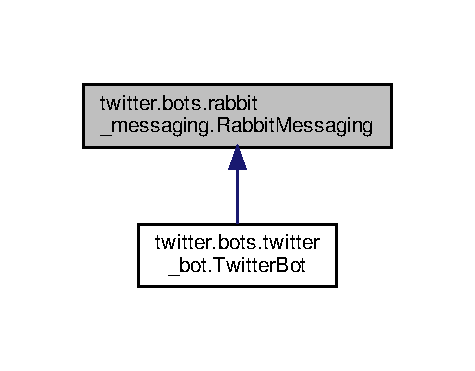
\includegraphics[width=228pt]{d9/d46/classtwitter_1_1bots_1_1rabbit__messaging_1_1RabbitMessaging__inherit__graph}
\end{center}
\end{figure}
\subsection*{Public Member Functions}
\begin{DoxyCompactItemize}
\item 
\mbox{\Hypertarget{classtwitter_1_1bots_1_1rabbit__messaging_1_1RabbitMessaging_a34c66d4ac88da28a2bd316ff79edf262}\label{classtwitter_1_1bots_1_1rabbit__messaging_1_1RabbitMessaging_a34c66d4ac88da28a2bd316ff79edf262}} 
def {\bfseries \+\_\+\+\_\+init\+\_\+\+\_\+}
\end{DoxyCompactItemize}
\subsection*{Public Attributes}
\begin{DoxyCompactItemize}
\item 
\mbox{\Hypertarget{classtwitter_1_1bots_1_1rabbit__messaging_1_1RabbitMessaging_a191a98366932a439235d21008d942267}\label{classtwitter_1_1bots_1_1rabbit__messaging_1_1RabbitMessaging_a191a98366932a439235d21008d942267}} 
{\bfseries vhost}
\item 
\mbox{\Hypertarget{classtwitter_1_1bots_1_1rabbit__messaging_1_1RabbitMessaging_a6b30781862012f4ca02c57b581e4561f}\label{classtwitter_1_1bots_1_1rabbit__messaging_1_1RabbitMessaging_a6b30781862012f4ca02c57b581e4561f}} 
{\bfseries settings}
\end{DoxyCompactItemize}
\subsection*{Private Member Functions}
\begin{DoxyCompactItemize}
\item 
def \hyperlink{classtwitter_1_1bots_1_1rabbit__messaging_1_1RabbitMessaging_aa1f0c32cb8d52910117c7db2a070a708}{\+\_\+\+\_\+reconnect\+\_\+messaging} (function)
\begin{DoxyCompactList}\small\item\em Decorator to try to reconnect multiple times if the connection to Rabbit\+MQ fails. \end{DoxyCompactList}\item 
\mbox{\Hypertarget{classtwitter_1_1bots_1_1rabbit__messaging_1_1RabbitMessaging_a3eb61ddf0a04971eb7ac7494bbc9012e}\label{classtwitter_1_1bots_1_1rabbit__messaging_1_1RabbitMessaging_a3eb61ddf0a04971eb7ac7494bbc9012e}} 
def {\bfseries \+\_\+\+\_\+connect} (self)
\item 
\mbox{\Hypertarget{classtwitter_1_1bots_1_1rabbit__messaging_1_1RabbitMessaging_a90cec3aa9d23d01e1bc04949226b2837}\label{classtwitter_1_1bots_1_1rabbit__messaging_1_1RabbitMessaging_a90cec3aa9d23d01e1bc04949226b2837}} 
def \hyperlink{classtwitter_1_1bots_1_1rabbit__messaging_1_1RabbitMessaging_a90cec3aa9d23d01e1bc04949226b2837}{\+\_\+setup\+\_\+messaging} (self)
\begin{DoxyCompactList}\small\item\em Private method for setting up the messaging connections. \end{DoxyCompactList}\item 
def \hyperlink{classtwitter_1_1bots_1_1rabbit__messaging_1_1RabbitMessaging_a82b3f62dcb3c12e53c03678128038832}{\+\_\+send\+\_\+message} (self, data, send\+\_\+to)
\begin{DoxyCompactList}\small\item\em Function to publish a message on one of the rabbit\+MQ\textquotesingle{}s exchanges. \end{DoxyCompactList}\item 
def \hyperlink{classtwitter_1_1bots_1_1rabbit__messaging_1_1RabbitMessaging_a9c1185869b76c0f456bda928697fec04}{\+\_\+receive\+\_\+message} (self, receive\+\_\+from)
\begin{DoxyCompactList}\small\item\em Function to get a message from a specific rabbit\+MQ exchange. \end{DoxyCompactList}\end{DoxyCompactItemize}
\subsection*{Private Attributes}
\begin{DoxyCompactItemize}
\item 
\mbox{\Hypertarget{classtwitter_1_1bots_1_1rabbit__messaging_1_1RabbitMessaging_af0701a7ad3de6c4dd98be35fa9d47a20}\label{classtwitter_1_1bots_1_1rabbit__messaging_1_1RabbitMessaging_af0701a7ad3de6c4dd98be35fa9d47a20}} 
{\bfseries \+\_\+\+\_\+url}
\item 
\mbox{\Hypertarget{classtwitter_1_1bots_1_1rabbit__messaging_1_1RabbitMessaging_a047b1f1a7ce84927fc0a160639ce7c6a}\label{classtwitter_1_1bots_1_1rabbit__messaging_1_1RabbitMessaging_a047b1f1a7ce84927fc0a160639ce7c6a}} 
{\bfseries \+\_\+\+\_\+username}
\item 
\mbox{\Hypertarget{classtwitter_1_1bots_1_1rabbit__messaging_1_1RabbitMessaging_af9b7145cb0f727efcaaff5cd53dc1247}\label{classtwitter_1_1bots_1_1rabbit__messaging_1_1RabbitMessaging_af9b7145cb0f727efcaaff5cd53dc1247}} 
{\bfseries \+\_\+\+\_\+password}
\item 
\mbox{\Hypertarget{classtwitter_1_1bots_1_1rabbit__messaging_1_1RabbitMessaging_a2884151e1f7af496aa9e1601224a25da}\label{classtwitter_1_1bots_1_1rabbit__messaging_1_1RabbitMessaging_a2884151e1f7af496aa9e1601224a25da}} 
{\bfseries \+\_\+\+\_\+reconnect\+\_\+max\+\_\+iterations}
\item 
\mbox{\Hypertarget{classtwitter_1_1bots_1_1rabbit__messaging_1_1RabbitMessaging_ac39e8e980f3c2b517b1a7e287938f2aa}\label{classtwitter_1_1bots_1_1rabbit__messaging_1_1RabbitMessaging_ac39e8e980f3c2b517b1a7e287938f2aa}} 
{\bfseries \+\_\+\+\_\+messaging}
\end{DoxyCompactItemize}


\subsection{Member Function Documentation}
\mbox{\Hypertarget{classtwitter_1_1bots_1_1rabbit__messaging_1_1RabbitMessaging_aa1f0c32cb8d52910117c7db2a070a708}\label{classtwitter_1_1bots_1_1rabbit__messaging_1_1RabbitMessaging_aa1f0c32cb8d52910117c7db2a070a708}} 
\index{twitter\+::bots\+::rabbit\+\_\+messaging\+::\+Rabbit\+Messaging@{twitter\+::bots\+::rabbit\+\_\+messaging\+::\+Rabbit\+Messaging}!\+\_\+\+\_\+reconnect\+\_\+messaging@{\+\_\+\+\_\+reconnect\+\_\+messaging}}
\index{\+\_\+\+\_\+reconnect\+\_\+messaging@{\+\_\+\+\_\+reconnect\+\_\+messaging}!twitter\+::bots\+::rabbit\+\_\+messaging\+::\+Rabbit\+Messaging@{twitter\+::bots\+::rabbit\+\_\+messaging\+::\+Rabbit\+Messaging}}
\subsubsection{\texorpdfstring{\+\_\+\+\_\+reconnect\+\_\+messaging()}{\_\_reconnect\_messaging()}}
{\footnotesize\ttfamily def twitter.\+bots.\+rabbit\+\_\+messaging.\+Rabbit\+Messaging.\+\_\+\+\_\+reconnect\+\_\+messaging (\begin{DoxyParamCaption}\item[{}]{function }\end{DoxyParamCaption})\hspace{0.3cm}{\ttfamily [private]}}



Decorator to try to reconnect multiple times if the connection to Rabbit\+MQ fails. 


\begin{DoxyParams}{Parameters}
{\em function} & () function to decorate \\
\hline
\end{DoxyParams}
\mbox{\Hypertarget{classtwitter_1_1bots_1_1rabbit__messaging_1_1RabbitMessaging_a9c1185869b76c0f456bda928697fec04}\label{classtwitter_1_1bots_1_1rabbit__messaging_1_1RabbitMessaging_a9c1185869b76c0f456bda928697fec04}} 
\index{twitter\+::bots\+::rabbit\+\_\+messaging\+::\+Rabbit\+Messaging@{twitter\+::bots\+::rabbit\+\_\+messaging\+::\+Rabbit\+Messaging}!\+\_\+receive\+\_\+message@{\+\_\+receive\+\_\+message}}
\index{\+\_\+receive\+\_\+message@{\+\_\+receive\+\_\+message}!twitter\+::bots\+::rabbit\+\_\+messaging\+::\+Rabbit\+Messaging@{twitter\+::bots\+::rabbit\+\_\+messaging\+::\+Rabbit\+Messaging}}
\subsubsection{\texorpdfstring{\+\_\+receive\+\_\+message()}{\_receive\_message()}}
{\footnotesize\ttfamily def twitter.\+bots.\+rabbit\+\_\+messaging.\+Rabbit\+Messaging.\+\_\+receive\+\_\+message (\begin{DoxyParamCaption}\item[{}]{self,  }\item[{}]{receive\+\_\+from }\end{DoxyParamCaption})\hspace{0.3cm}{\ttfamily [private]}}



Function to get a message from a specific rabbit\+MQ exchange. 


\begin{DoxyParams}{Parameters}
{\em receive\+\_\+from} & (str) where to get the data; corresponds to a str key in self.\+settings, where that key maps to an object with the exchange and routing key values \\
\hline
\end{DoxyParams}
\mbox{\Hypertarget{classtwitter_1_1bots_1_1rabbit__messaging_1_1RabbitMessaging_a82b3f62dcb3c12e53c03678128038832}\label{classtwitter_1_1bots_1_1rabbit__messaging_1_1RabbitMessaging_a82b3f62dcb3c12e53c03678128038832}} 
\index{twitter\+::bots\+::rabbit\+\_\+messaging\+::\+Rabbit\+Messaging@{twitter\+::bots\+::rabbit\+\_\+messaging\+::\+Rabbit\+Messaging}!\+\_\+send\+\_\+message@{\+\_\+send\+\_\+message}}
\index{\+\_\+send\+\_\+message@{\+\_\+send\+\_\+message}!twitter\+::bots\+::rabbit\+\_\+messaging\+::\+Rabbit\+Messaging@{twitter\+::bots\+::rabbit\+\_\+messaging\+::\+Rabbit\+Messaging}}
\subsubsection{\texorpdfstring{\+\_\+send\+\_\+message()}{\_send\_message()}}
{\footnotesize\ttfamily def twitter.\+bots.\+rabbit\+\_\+messaging.\+Rabbit\+Messaging.\+\_\+send\+\_\+message (\begin{DoxyParamCaption}\item[{}]{self,  }\item[{}]{data,  }\item[{}]{send\+\_\+to }\end{DoxyParamCaption})\hspace{0.3cm}{\ttfamily [private]}}



Function to publish a message on one of the rabbit\+MQ\textquotesingle{}s exchanges. 


\begin{DoxyParams}{Parameters}
{\em data} & (json) data to publish in json format \\
\hline
{\em send\+\_\+to} & (str) where to publish the data; corresponds to a str key in self.\+settings, where that key maps to an object with the exchange and routing key values \\
\hline
\end{DoxyParams}


The documentation for this class was generated from the following file\+:\begin{DoxyCompactItemize}
\item 
bots/rabbit\+\_\+messaging.\+py\end{DoxyCompactItemize}

\hypertarget{classtwitter_1_1wrappers_1_1rabbitmq__wrapper_1_1Rabbitmq}{}\section{twitter.\+wrappers.\+rabbitmq\+\_\+wrapper.\+Rabbitmq Class Reference}
\label{classtwitter_1_1wrappers_1_1rabbitmq__wrapper_1_1Rabbitmq}\index{twitter.\+wrappers.\+rabbitmq\+\_\+wrapper.\+Rabbitmq@{twitter.\+wrappers.\+rabbitmq\+\_\+wrapper.\+Rabbitmq}}


Class representing Rabbit MQ.  




Inheritance diagram for twitter.\+wrappers.\+rabbitmq\+\_\+wrapper.\+Rabbitmq\+:
\nopagebreak
\begin{figure}[H]
\begin{center}
\leavevmode
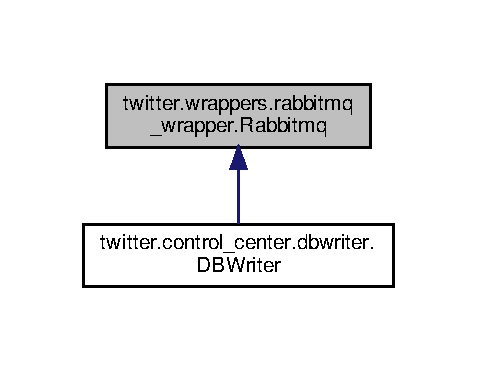
\includegraphics[width=229pt]{da/d15/classtwitter_1_1wrappers_1_1rabbitmq__wrapper_1_1Rabbitmq__inherit__graph}
\end{center}
\end{figure}
\subsection*{Public Member Functions}
\begin{DoxyCompactItemize}
\item 
def \hyperlink{classtwitter_1_1wrappers_1_1rabbitmq__wrapper_1_1Rabbitmq_a62d86eb0c3c5f086500ef0097f9efd65}{\+\_\+\+\_\+init\+\_\+\+\_\+} (self, host=R\+A\+B\+B\+I\+T\+M\+Q\+\_\+\+U\+RL, port=R\+A\+B\+B\+I\+T\+M\+Q\+\_\+\+P\+O\+RT, vhost=V\+H\+O\+ST, username=R\+A\+B\+B\+I\+T\+M\+Q\+\_\+\+U\+S\+E\+R\+N\+A\+ME, pika\+\_\+credentials=pika.\+Plain\+Credentials(username, password) self.\+pika\+\_\+parameters=pika.\+Connection\+Parameters(host=host, port=port, virtual\+\_\+host=vhost, credentials=pika\+\_\+credentials, heartbeat=600, blocked\+\_\+connection\+\_\+timeout=300) self.\+reconnection\+\_\+attempt=0 self.\+M\+A\+X\+\_\+\+R\+E\+C\+O\+N\+N\+E\+C\+T\+I\+O\+NS=10 self.\+connection=None self.\+channel=None self.\+\_\+\+\_\+setup() \#\# \# Set up function, will, start, the, connection, create, all, necessary, exchanges, and, respective, bindings, from, the, def, \+\_\+\+\_\+setup, self)
\begin{DoxyCompactList}\small\item\em Create a Rabbit MQ instance which represents a connection to a Rabbit MQ server. \end{DoxyCompactList}\item 
\mbox{\Hypertarget{classtwitter_1_1wrappers_1_1rabbitmq__wrapper_1_1Rabbitmq_a910cadec1f119ffca78becc55af22a43}\label{classtwitter_1_1wrappers_1_1rabbitmq__wrapper_1_1Rabbitmq_a910cadec1f119ffca78becc55af22a43}} 
def \hyperlink{classtwitter_1_1wrappers_1_1rabbitmq__wrapper_1_1Rabbitmq_a910cadec1f119ffca78becc55af22a43}{received\+\_\+message\+\_\+handler} (self, channel, method, properties, body)
\begin{DoxyCompactList}\small\item\em Function to rewrite on the class that inherits this class. \end{DoxyCompactList}\end{DoxyCompactItemize}
\subsection*{Public Attributes}
\begin{DoxyCompactItemize}
\item 
\mbox{\Hypertarget{classtwitter_1_1wrappers_1_1rabbitmq__wrapper_1_1Rabbitmq_aa9419b8984be09e42873e11572e93139}\label{classtwitter_1_1wrappers_1_1rabbitmq__wrapper_1_1Rabbitmq_aa9419b8984be09e42873e11572e93139}} 
{\bfseries connection}
\item 
\mbox{\Hypertarget{classtwitter_1_1wrappers_1_1rabbitmq__wrapper_1_1Rabbitmq_a049721cef6898206c8e6dab244b144fd}\label{classtwitter_1_1wrappers_1_1rabbitmq__wrapper_1_1Rabbitmq_a049721cef6898206c8e6dab244b144fd}} 
{\bfseries channel}
\end{DoxyCompactItemize}
\subsection*{Private Member Functions}
\begin{DoxyCompactItemize}
\item 
def \hyperlink{classtwitter_1_1wrappers_1_1rabbitmq__wrapper_1_1Rabbitmq_aff19e59d7fd9025f21972e331a1fdfde}{\+\_\+send} (self, routing\+\_\+key, message)
\begin{DoxyCompactList}\small\item\em Routes the message to corresponding channel. \end{DoxyCompactList}\item 
def \hyperlink{classtwitter_1_1wrappers_1_1rabbitmq__wrapper_1_1Rabbitmq_a430a4af33557422e4a0575323b6d7027}{\+\_\+receive} (self, queue\+\_\+name=\textquotesingle{}A\+PI\textquotesingle{})
\begin{DoxyCompactList}\small\item\em Receives messages and puts them in the queue given from the argument. \end{DoxyCompactList}\item 
\mbox{\Hypertarget{classtwitter_1_1wrappers_1_1rabbitmq__wrapper_1_1Rabbitmq_aeb0b7d3eee2a07ca9b795924e2af584c}\label{classtwitter_1_1wrappers_1_1rabbitmq__wrapper_1_1Rabbitmq_aeb0b7d3eee2a07ca9b795924e2af584c}} 
def \hyperlink{classtwitter_1_1wrappers_1_1rabbitmq__wrapper_1_1Rabbitmq_aeb0b7d3eee2a07ca9b795924e2af584c}{\+\_\+close} (self)
\begin{DoxyCompactList}\small\item\em Close the connection with the Rabbit MQ server. \end{DoxyCompactList}\end{DoxyCompactItemize}


\subsection{Detailed Description}
Class representing Rabbit MQ. 

\subsection{Constructor \& Destructor Documentation}
\mbox{\Hypertarget{classtwitter_1_1wrappers_1_1rabbitmq__wrapper_1_1Rabbitmq_a62d86eb0c3c5f086500ef0097f9efd65}\label{classtwitter_1_1wrappers_1_1rabbitmq__wrapper_1_1Rabbitmq_a62d86eb0c3c5f086500ef0097f9efd65}} 
\index{twitter\+::wrappers\+::rabbitmq\+\_\+wrapper\+::\+Rabbitmq@{twitter\+::wrappers\+::rabbitmq\+\_\+wrapper\+::\+Rabbitmq}!\+\_\+\+\_\+init\+\_\+\+\_\+@{\+\_\+\+\_\+init\+\_\+\+\_\+}}
\index{\+\_\+\+\_\+init\+\_\+\+\_\+@{\+\_\+\+\_\+init\+\_\+\+\_\+}!twitter\+::wrappers\+::rabbitmq\+\_\+wrapper\+::\+Rabbitmq@{twitter\+::wrappers\+::rabbitmq\+\_\+wrapper\+::\+Rabbitmq}}
\subsubsection{\texorpdfstring{\+\_\+\+\_\+init\+\_\+\+\_\+()}{\_\_init\_\_()}}
{\footnotesize\ttfamily def twitter.\+wrappers.\+rabbitmq\+\_\+wrapper.\+Rabbitmq.\+\_\+\+\_\+init\+\_\+\+\_\+ (\begin{DoxyParamCaption}\item[{}]{self,  }\item[{}]{host = {\ttfamily RABBITMQ\+\_\+URL},  }\item[{}]{port = {\ttfamily RABBITMQ\+\_\+PORT},  }\item[{}]{vhost = {\ttfamily VHOST},  }\item[{}]{username = {\ttfamily RABBITMQ\+\_\+USERNAME},  }\item[{}]{pika\+\_\+credentials = {\ttfamily pika.PlainCredentials(username,~password)
~~~~~~~~self.pika\+\_\+parameters~=~pika.ConnectionParameters(
~~~~~~~~~~~~host=host,
~~~~~~~~~~~~port=port,
~~~~~~~~~~~~virtual\+\_\+host=vhost,
~~~~~~~~~~~~credentials=pika\+\_\+credentials,
~~~~~~~~~~~~heartbeat=600,
~~~~~~~~~~~~blocked\+\_\+connection\+\_\+timeout=300
~~~~~~~~)

~~~~~~~~self.reconnection\+\_\+attempt~=~0
~~~~~~~~self.MAX\+\_\+RECONNECTIONS~=~10
~~~~~~~~self.connection~=~None
~~~~~~~~self.channel~=~None
~~~~~~~~self.\+\_\+\+\_\+setup()
~~~~
~~~~\#\#~~~~~~~~~
~~~~\#~~~~~~~~~Set~up~function},  }\item[{}]{will,  }\item[{}]{start,  }\item[{}]{the,  }\item[{}]{connection,  }\item[{}]{create,  }\item[{}]{all,  }\item[{}]{necessary,  }\item[{}]{exchanges,  }\item[{}]{and,  }\item[{}]{respective,  }\item[{}]{bindings,  }\item[{}]{from,  }\item[{}]{the,  }\item[{}]{def,  }\item[{}]{\+\_\+\+\_\+setup,  }\item[{}]{self }\end{DoxyParamCaption})}



Create a Rabbit MQ instance which represents a connection to a Rabbit MQ server. 

\subsubsection*{Parameters }

host \+: str Hostname port \+: int Port Number vhost \+: str Virtual host used to avoid conflicts between instances username \+: str Username for authentication password \+: str Password for authentication 

\subsection{Member Function Documentation}
\mbox{\Hypertarget{classtwitter_1_1wrappers_1_1rabbitmq__wrapper_1_1Rabbitmq_a430a4af33557422e4a0575323b6d7027}\label{classtwitter_1_1wrappers_1_1rabbitmq__wrapper_1_1Rabbitmq_a430a4af33557422e4a0575323b6d7027}} 
\index{twitter\+::wrappers\+::rabbitmq\+\_\+wrapper\+::\+Rabbitmq@{twitter\+::wrappers\+::rabbitmq\+\_\+wrapper\+::\+Rabbitmq}!\+\_\+receive@{\+\_\+receive}}
\index{\+\_\+receive@{\+\_\+receive}!twitter\+::wrappers\+::rabbitmq\+\_\+wrapper\+::\+Rabbitmq@{twitter\+::wrappers\+::rabbitmq\+\_\+wrapper\+::\+Rabbitmq}}
\subsubsection{\texorpdfstring{\+\_\+receive()}{\_receive()}}
{\footnotesize\ttfamily def twitter.\+wrappers.\+rabbitmq\+\_\+wrapper.\+Rabbitmq.\+\_\+receive (\begin{DoxyParamCaption}\item[{}]{self,  }\item[{}]{queue\+\_\+name = {\ttfamily \textquotesingle{}API\textquotesingle{}} }\end{DoxyParamCaption})\hspace{0.3cm}{\ttfamily [private]}}



Receives messages and puts them in the queue given from the argument. 

\subsubsection*{params\+: }

queue\+\_\+name \+: (string) Name of the queue to be declared \mbox{\Hypertarget{classtwitter_1_1wrappers_1_1rabbitmq__wrapper_1_1Rabbitmq_aff19e59d7fd9025f21972e331a1fdfde}\label{classtwitter_1_1wrappers_1_1rabbitmq__wrapper_1_1Rabbitmq_aff19e59d7fd9025f21972e331a1fdfde}} 
\index{twitter\+::wrappers\+::rabbitmq\+\_\+wrapper\+::\+Rabbitmq@{twitter\+::wrappers\+::rabbitmq\+\_\+wrapper\+::\+Rabbitmq}!\+\_\+send@{\+\_\+send}}
\index{\+\_\+send@{\+\_\+send}!twitter\+::wrappers\+::rabbitmq\+\_\+wrapper\+::\+Rabbitmq@{twitter\+::wrappers\+::rabbitmq\+\_\+wrapper\+::\+Rabbitmq}}
\subsubsection{\texorpdfstring{\+\_\+send()}{\_send()}}
{\footnotesize\ttfamily def twitter.\+wrappers.\+rabbitmq\+\_\+wrapper.\+Rabbitmq.\+\_\+send (\begin{DoxyParamCaption}\item[{}]{self,  }\item[{}]{routing\+\_\+key,  }\item[{}]{message }\end{DoxyParamCaption})\hspace{0.3cm}{\ttfamily [private]}}



Routes the message to corresponding channel. 

\subsubsection*{params\+: }

routing\+\_\+key\+: (string) routing key to bding to queue message\+: (Dictionary) dictionary to be stringified and sent 

The documentation for this class was generated from the following file\+:\begin{DoxyCompactItemize}
\item 
wrappers/rabbitmq\+\_\+wrapper.\+py\end{DoxyCompactItemize}

\hypertarget{classtwitter_1_1control__center_1_1enums_1_1ResponseTypes}{}\section{twitter.\+control\+\_\+center.\+enums.\+Response\+Types Class Reference}
\label{classtwitter_1_1control__center_1_1enums_1_1ResponseTypes}\index{twitter.\+control\+\_\+center.\+enums.\+Response\+Types@{twitter.\+control\+\_\+center.\+enums.\+Response\+Types}}


Inheritance diagram for twitter.\+control\+\_\+center.\+enums.\+Response\+Types\+:\nopagebreak
\begin{figure}[H]
\begin{center}
\leavevmode
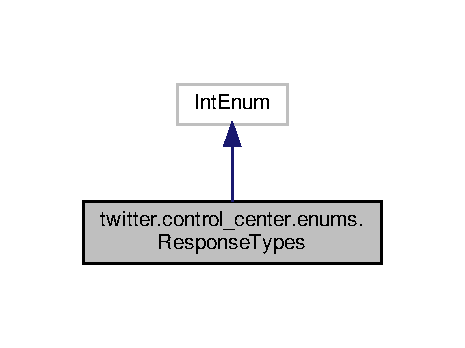
\includegraphics[width=223pt]{classtwitter_1_1control__center_1_1enums_1_1ResponseTypes__inherit__graph}
\end{center}
\end{figure}


Collaboration diagram for twitter.\+control\+\_\+center.\+enums.\+Response\+Types\+:\nopagebreak
\begin{figure}[H]
\begin{center}
\leavevmode
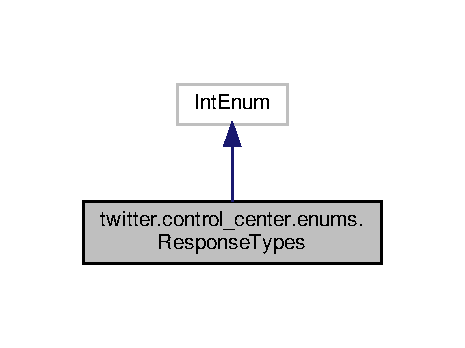
\includegraphics[width=223pt]{classtwitter_1_1control__center_1_1enums_1_1ResponseTypes__coll__graph}
\end{center}
\end{figure}
\subsection*{Static Public Attributes}
\begin{DoxyCompactItemize}
\item 
\mbox{\Hypertarget{classtwitter_1_1control__center_1_1enums_1_1ResponseTypes_ae730dee107c0ceced428c11c89d3cf55}\label{classtwitter_1_1control__center_1_1enums_1_1ResponseTypes_ae730dee107c0ceced428c11c89d3cf55}} 
int {\bfseries F\+O\+L\+L\+O\+W\+\_\+\+U\+S\+E\+RS} = 1
\item 
\mbox{\Hypertarget{classtwitter_1_1control__center_1_1enums_1_1ResponseTypes_ad981b4a159fa5c0ac5ada90e1165099c}\label{classtwitter_1_1control__center_1_1enums_1_1ResponseTypes_ad981b4a159fa5c0ac5ada90e1165099c}} 
int {\bfseries F\+I\+N\+D\+\_\+\+B\+Y\+\_\+\+K\+E\+Y\+W\+O\+R\+DS} = 2
\item 
\mbox{\Hypertarget{classtwitter_1_1control__center_1_1enums_1_1ResponseTypes_a7b85cfde98eff7d69ec16d6bc6f019cf}\label{classtwitter_1_1control__center_1_1enums_1_1ResponseTypes_a7b85cfde98eff7d69ec16d6bc6f019cf}} 
int {\bfseries L\+I\+K\+E\+\_\+\+T\+W\+E\+E\+TS} = 3
\item 
\mbox{\Hypertarget{classtwitter_1_1control__center_1_1enums_1_1ResponseTypes_a29f6317f18e2560582a7c0e4d57ffaa2}\label{classtwitter_1_1control__center_1_1enums_1_1ResponseTypes_a29f6317f18e2560582a7c0e4d57ffaa2}} 
int {\bfseries R\+E\+T\+W\+E\+E\+T\+\_\+\+T\+W\+E\+E\+TS} = 4
\item 
\mbox{\Hypertarget{classtwitter_1_1control__center_1_1enums_1_1ResponseTypes_aea9068ca1d2140ce2ffd41d2609141f6}\label{classtwitter_1_1control__center_1_1enums_1_1ResponseTypes_aea9068ca1d2140ce2ffd41d2609141f6}} 
int {\bfseries P\+O\+S\+T\+\_\+\+T\+W\+E\+E\+TS} = 5
\item 
\mbox{\Hypertarget{classtwitter_1_1control__center_1_1enums_1_1ResponseTypes_add3b1e9f25232e004ee2cd9977d39782}\label{classtwitter_1_1control__center_1_1enums_1_1ResponseTypes_add3b1e9f25232e004ee2cd9977d39782}} 
int {\bfseries F\+I\+N\+D\+\_\+\+F\+O\+L\+L\+O\+W\+E\+RS} = 6
\end{DoxyCompactItemize}


The documentation for this class was generated from the following file\+:\begin{DoxyCompactItemize}
\item 
control\+\_\+center/enums.\+py\end{DoxyCompactItemize}

\hypertarget{classtwitter_1_1bots_1_1messages__types_1_1ServerToBot}{}\section{twitter.\+bots.\+messages\+\_\+types.\+Server\+To\+Bot Class Reference}
\label{classtwitter_1_1bots_1_1messages__types_1_1ServerToBot}\index{twitter.\+bots.\+messages\+\_\+types.\+Server\+To\+Bot@{twitter.\+bots.\+messages\+\_\+types.\+Server\+To\+Bot}}


Inheritance diagram for twitter.\+bots.\+messages\+\_\+types.\+Server\+To\+Bot\+:
\nopagebreak
\begin{figure}[H]
\begin{center}
\leavevmode
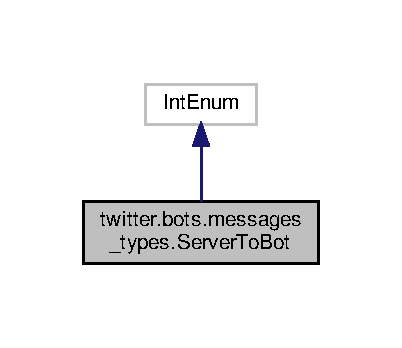
\includegraphics[width=193pt]{classtwitter_1_1bots_1_1messages__types_1_1ServerToBot__inherit__graph}
\end{center}
\end{figure}


Collaboration diagram for twitter.\+bots.\+messages\+\_\+types.\+Server\+To\+Bot\+:
\nopagebreak
\begin{figure}[H]
\begin{center}
\leavevmode
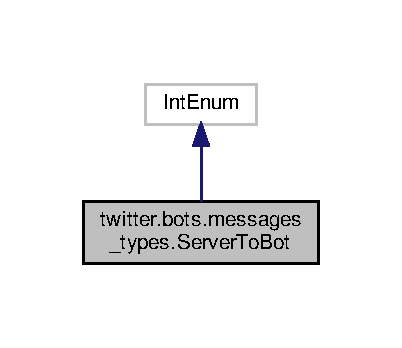
\includegraphics[width=193pt]{classtwitter_1_1bots_1_1messages__types_1_1ServerToBot__coll__graph}
\end{center}
\end{figure}
\subsection*{Public Member Functions}
\begin{DoxyCompactItemize}
\item 
\mbox{\Hypertarget{classtwitter_1_1bots_1_1messages__types_1_1ServerToBot_a985e5ee49b6d8aec3555283ca6bf2f28}\label{classtwitter_1_1bots_1_1messages__types_1_1ServerToBot_a985e5ee49b6d8aec3555283ca6bf2f28}} 
def {\bfseries \+\_\+\+\_\+str\+\_\+\+\_\+} (self)
\end{DoxyCompactItemize}
\subsection*{Static Public Attributes}
\begin{DoxyCompactItemize}
\item 
\mbox{\Hypertarget{classtwitter_1_1bots_1_1messages__types_1_1ServerToBot_a88d7b857870002d072fe166c5470b57c}\label{classtwitter_1_1bots_1_1messages__types_1_1ServerToBot_a88d7b857870002d072fe166c5470b57c}} 
int {\bfseries F\+O\+L\+L\+O\+W\+\_\+\+U\+S\+E\+RS} = 1
\item 
\mbox{\Hypertarget{classtwitter_1_1bots_1_1messages__types_1_1ServerToBot_ab8ff4adb87b0a82e4a4d3a9d4872218f}\label{classtwitter_1_1bots_1_1messages__types_1_1ServerToBot_ab8ff4adb87b0a82e4a4d3a9d4872218f}} 
int {\bfseries F\+I\+N\+D\+\_\+\+B\+Y\+\_\+\+K\+E\+Y\+W\+O\+R\+DS} = 2
\item 
\mbox{\Hypertarget{classtwitter_1_1bots_1_1messages__types_1_1ServerToBot_ae2b672776672a89efd18c364aa5863e6}\label{classtwitter_1_1bots_1_1messages__types_1_1ServerToBot_ae2b672776672a89efd18c364aa5863e6}} 
int {\bfseries L\+I\+K\+E\+\_\+\+T\+W\+E\+E\+TS} = 3
\item 
\mbox{\Hypertarget{classtwitter_1_1bots_1_1messages__types_1_1ServerToBot_acc229477b6b55292309f5da7a305dfd0}\label{classtwitter_1_1bots_1_1messages__types_1_1ServerToBot_acc229477b6b55292309f5da7a305dfd0}} 
int {\bfseries R\+E\+T\+W\+E\+E\+T\+\_\+\+T\+W\+E\+E\+TS} = 4
\item 
\mbox{\Hypertarget{classtwitter_1_1bots_1_1messages__types_1_1ServerToBot_a3b4fe80ad0c9c0ff7877174cab41fa97}\label{classtwitter_1_1bots_1_1messages__types_1_1ServerToBot_a3b4fe80ad0c9c0ff7877174cab41fa97}} 
int {\bfseries P\+O\+S\+T\+\_\+\+T\+W\+E\+ET} = 5
\item 
\mbox{\Hypertarget{classtwitter_1_1bots_1_1messages__types_1_1ServerToBot_ac1549a314813b403ecda2b7ead3c56c6}\label{classtwitter_1_1bots_1_1messages__types_1_1ServerToBot_ac1549a314813b403ecda2b7ead3c56c6}} 
int {\bfseries F\+I\+N\+D\+\_\+\+F\+O\+L\+L\+O\+W\+E\+RS} = 6
\end{DoxyCompactItemize}


\subsection{Detailed Description}
\begin{DoxyVerb}Enum for the tasks the bot is able to run. Received by the bot from the server.
\end{DoxyVerb}
 

The documentation for this class was generated from the following file\+:\begin{DoxyCompactItemize}
\item 
bots/messages\+\_\+types.\+py\end{DoxyCompactItemize}

\hypertarget{classtwitter_1_1bots_1_1twitter__bot_1_1TwitterBot}{}\section{twitter.\+bots.\+twitter\+\_\+bot.\+Twitter\+Bot Class Reference}
\label{classtwitter_1_1bots_1_1twitter__bot_1_1TwitterBot}\index{twitter.\+bots.\+twitter\+\_\+bot.\+Twitter\+Bot@{twitter.\+bots.\+twitter\+\_\+bot.\+Twitter\+Bot}}


Inheritance diagram for twitter.\+bots.\+twitter\+\_\+bot.\+Twitter\+Bot\+:
\nopagebreak
\begin{figure}[H]
\begin{center}
\leavevmode
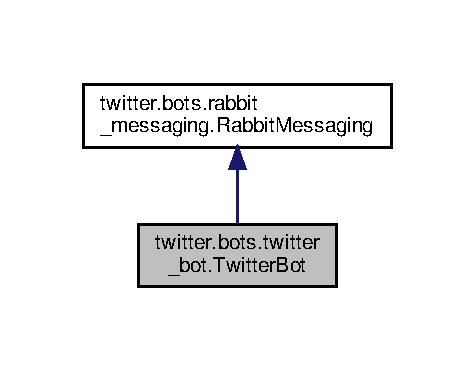
\includegraphics[width=228pt]{classtwitter_1_1bots_1_1twitter__bot_1_1TwitterBot__inherit__graph}
\end{center}
\end{figure}


Collaboration diagram for twitter.\+bots.\+twitter\+\_\+bot.\+Twitter\+Bot\+:
\nopagebreak
\begin{figure}[H]
\begin{center}
\leavevmode
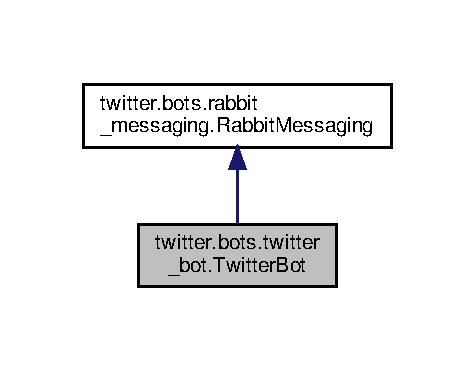
\includegraphics[width=228pt]{classtwitter_1_1bots_1_1twitter__bot_1_1TwitterBot__coll__graph}
\end{center}
\end{figure}
\subsection*{Public Member Functions}
\begin{DoxyCompactItemize}
\item 
\mbox{\Hypertarget{classtwitter_1_1bots_1_1twitter__bot_1_1TwitterBot_a19e4ba96300342dd63980717852a30b3}\label{classtwitter_1_1bots_1_1twitter__bot_1_1TwitterBot_a19e4ba96300342dd63980717852a30b3}} 
def {\bfseries \+\_\+\+\_\+init\+\_\+\+\_\+}
\item 
\mbox{\Hypertarget{classtwitter_1_1bots_1_1twitter__bot_1_1TwitterBot_a599499bf98dd54aeb95938c18086477f}\label{classtwitter_1_1bots_1_1twitter__bot_1_1TwitterBot_a599499bf98dd54aeb95938c18086477f}} 
def {\bfseries \+\_\+\+\_\+repr\+\_\+\+\_\+} (self)
\item 
def \hyperlink{classtwitter_1_1bots_1_1twitter__bot_1_1TwitterBot_aa0425e1810fa53dab90ca0e9d7b973d1}{run} (self)
\end{DoxyCompactItemize}
\subsection*{Public Attributes}
\begin{DoxyCompactItemize}
\item 
\mbox{\Hypertarget{classtwitter_1_1bots_1_1twitter__bot_1_1TwitterBot_af7ed1ab8062dc7e29dbf8ced90b6ca3c}\label{classtwitter_1_1bots_1_1twitter__bot_1_1TwitterBot_af7ed1ab8062dc7e29dbf8ced90b6ca3c}} 
{\bfseries user}
\end{DoxyCompactItemize}


\subsection{Member Function Documentation}
\mbox{\Hypertarget{classtwitter_1_1bots_1_1twitter__bot_1_1TwitterBot_aa0425e1810fa53dab90ca0e9d7b973d1}\label{classtwitter_1_1bots_1_1twitter__bot_1_1TwitterBot_aa0425e1810fa53dab90ca0e9d7b973d1}} 
\index{twitter\+::bots\+::twitter\+\_\+bot\+::\+Twitter\+Bot@{twitter\+::bots\+::twitter\+\_\+bot\+::\+Twitter\+Bot}!run@{run}}
\index{run@{run}!twitter\+::bots\+::twitter\+\_\+bot\+::\+Twitter\+Bot@{twitter\+::bots\+::twitter\+\_\+bot\+::\+Twitter\+Bot}}
\subsubsection{\texorpdfstring{run()}{run()}}
{\footnotesize\ttfamily def twitter.\+bots.\+twitter\+\_\+bot.\+Twitter\+Bot.\+run (\begin{DoxyParamCaption}\item[{}]{self }\end{DoxyParamCaption})}

\begin{DoxyVerb}Bot's loop. As simple as a normal handler, tries to get tasks from the queue and, depending on the
    task, does a different action
\end{DoxyVerb}
 

The documentation for this class was generated from the following file\+:\begin{DoxyCompactItemize}
\item 
bots/twitter\+\_\+bot.\+py\end{DoxyCompactItemize}

%--- End generated contents ---

% Index
\backmatter
\newpage
\phantomsection
\clearemptydoublepage
\addcontentsline{toc}{chapter}{Index}
\printindex

\end{document}
